\documentclass{article}


% if you need to pass options to natbib, use, e.g.:
\PassOptionsToPackage{numbers, compress}{natbib}
% before loading neurips_2024


% ready for submission
\usepackage[final]{neurips_2024}


% to compile a preprint version, e.g., for submission to arXiv, add add the
% [preprint] option:
%     \usepackage[preprint]{neurips_2024}


% to compile a camera-ready version, add the [final] option, e.g.:
%     \usepackage[final]{neurips_2024}


% to avoid loading the natbib package, add option nonatbib:
%     \usepackage[nonatbib]{neurips_2024}


\usepackage[utf8]{inputenc} % allow utf-8 input
\usepackage[T1]{fontenc}    % use 8-bit T1 fonts
\usepackage{hyperref}       % hyperlinks
\usepackage{url}            % simple URL typesetting
\usepackage{booktabs}       % professional-quality tables
\usepackage{amsfonts}       % blackboard math symbols
\usepackage{nicefrac}       % compact symbols for 1/2, etc.

\usepackage{lipsum}         %
\usepackage{todonotes}
\usepackage{subfigure}
\usepackage{algorithm}
% \usepackage{algorithmic}
\usepackage{algpseudocode}
\usepackage{tabulary}

\usepackage{xcolor}         % colors
\usepackage{microtype}
\usepackage{hyperref}
\usepackage{url}
\usepackage{booktabs}
\usepackage{microtype}
\usepackage{booktabs} % for professional tables
\usepackage{tabularray}
\usepackage{graphicx}
\usepackage{amsmath}
\usepackage{amssymb}
\usepackage{mathtools}
\usepackage{amsthm}
\usepackage{wrapfig}
\usepackage{float}
\usepackage{subcaption}
\usepackage{enumitem}
% \usepackage{geometry}
\usepackage{verbatim}
\usepackage{tcolorbox}
\usepackage{soul}
\usepackage{listings}

\usepackage{amssymb}%
\usepackage{pifont}%

% for appendix toc
\usepackage{minitoc}
\usepackage{booktabs}   

%%%%% NEW MATH DEFINITIONS %%%%%

\usepackage{amsmath,amsfonts,bm}


\newcommand{\ret}{\mathbf{R}}
\newcommand{\emb}{\mathbf{E}}
\newcommand{\llm}{\mathbf{M}}

\newcommand{\topic}{PLfB}
\newcommand{\algo}{URI}

\newcommand{\rewf}{R}
\newcommand{\transf}{T}

\newcommand{\know}{\mathcal{K}}
\newcommand{\books}{\mathcal{B}}

% Mark sections of captions for referring to divisions of figures
\newcommand{\figleft}{{\em (Left)}}
\newcommand{\figcenter}{{\em (Center)}}
\newcommand{\figright}{{\em (Right)}}
\newcommand{\figtop}{{\em (Top)}}
\newcommand{\figbottom}{{\em (Bottom)}}
\newcommand{\captiona}{{\em (a)}}
\newcommand{\captionb}{{\em (b)}}
\newcommand{\captionc}{{\em (c)}}
\newcommand{\captiond}{{\em (d)}}

% Highlight a newly defined term
\newcommand{\newterm}[1]{{\bf #1}}


% Figure reference, lower-case.
\def\figref#1{figure~\ref{#1}}
% Figure reference, capital. For start of sentence
\def\Figref#1{Figure~\ref{#1}}
\def\twofigref#1#2{figures \ref{#1} and \ref{#2}}
\def\quadfigref#1#2#3#4{figures \ref{#1}, \ref{#2}, \ref{#3} and \ref{#4}}
% Section reference, lower-case.
\def\secref#1{section~\ref{#1}}
% Section reference, capital.
\def\Secref#1{Section~\ref{#1}}
% Reference to two sections.
\def\twosecrefs#1#2{sections \ref{#1} and \ref{#2}}
% Reference to three sections.
\def\secrefs#1#2#3{sections \ref{#1}, \ref{#2} and \ref{#3}}
% Reference to an equation, lower-case.
\def\eqref#1{equation~\ref{#1}}
% Reference to an equation, upper case
\def\Eqref#1{Equation~\ref{#1}}
% A raw reference to an equation---avoid using if possible
\def\plaineqref#1{\ref{#1}}
% Reference to a chapter, lower-case.
\def\chapref#1{chapter~\ref{#1}}
% Reference to an equation, upper case.
\def\Chapref#1{Chapter~\ref{#1}}
% Reference to a range of chapters
\def\rangechapref#1#2{chapters\ref{#1}--\ref{#2}}
% Reference to an algorithm, lower-case.
\def\algref#1{algorithm~\ref{#1}}
% Reference to an algorithm, upper case.
\def\Algref#1{Algorithm~\ref{#1}}
\def\twoalgref#1#2{algorithms \ref{#1} and \ref{#2}}
\def\Twoalgref#1#2{Algorithms \ref{#1} and \ref{#2}}
% Reference to a part, lower case
\def\partref#1{part~\ref{#1}}
% Reference to a part, upper case
\def\Partref#1{Part~\ref{#1}}
\def\twopartref#1#2{parts \ref{#1} and \ref{#2}}

\def\ceil#1{\lceil #1 \rceil}
\def\floor#1{\lfloor #1 \rfloor}
\def\1{\bm{1}}
\newcommand{\train}{\mathcal{D}}
\newcommand{\valid}{\mathcal{D_{\mathrm{valid}}}}
\newcommand{\test}{\mathcal{D_{\mathrm{test}}}}

\def\eps{{\epsilon}}


% Random variables
\def\reta{{\textnormal{$\eta$}}}
\def\ra{{\textnormal{a}}}
\def\rb{{\textnormal{b}}}
\def\rc{{\textnormal{c}}}
\def\rd{{\textnormal{d}}}
\def\re{{\textnormal{e}}}
\def\rf{{\textnormal{f}}}
\def\rg{{\textnormal{g}}}
\def\rh{{\textnormal{h}}}
\def\ri{{\textnormal{i}}}
\def\rj{{\textnormal{j}}}
\def\rk{{\textnormal{k}}}
\def\rl{{\textnormal{l}}}
% rm is already a command, just don't name any random variables m
\def\rn{{\textnormal{n}}}
\def\ro{{\textnormal{o}}}
\def\rp{{\textnormal{p}}}
\def\rq{{\textnormal{q}}}
\def\rr{{\textnormal{r}}}
\def\rs{{\textnormal{s}}}
\def\rt{{\textnormal{t}}}
\def\ru{{\textnormal{u}}}
\def\rv{{\textnormal{v}}}
\def\rw{{\textnormal{w}}}
\def\rx{{\textnormal{x}}}
\def\ry{{\textnormal{y}}}
\def\rz{{\textnormal{z}}}

% Random vectors
\def\rvepsilon{{\mathbf{\epsilon}}}
\def\rvtheta{{\mathbf{\theta}}}
\def\rva{{\mathbf{a}}}
\def\rvb{{\mathbf{b}}}
\def\rvc{{\mathbf{c}}}
\def\rvd{{\mathbf{d}}}
\def\rve{{\mathbf{e}}}
\def\rvf{{\mathbf{f}}}
\def\rvg{{\mathbf{g}}}
\def\rvh{{\mathbf{h}}}
\def\rvu{{\mathbf{i}}}
\def\rvj{{\mathbf{j}}}
\def\rvk{{\mathbf{k}}}
\def\rvl{{\mathbf{l}}}
\def\rvm{{\mathbf{m}}}
\def\rvn{{\mathbf{n}}}
\def\rvo{{\mathbf{o}}}
\def\rvp{{\mathbf{p}}}
\def\rvq{{\mathbf{q}}}
\def\rvr{{\mathbf{r}}}
\def\rvs{{\mathbf{s}}}
\def\rvt{{\mathbf{t}}}
\def\rvu{{\mathbf{u}}}
\def\rvv{{\mathbf{v}}}
\def\rvw{{\mathbf{w}}}
\def\rvx{{\mathbf{x}}}
\def\rvy{{\mathbf{y}}}
\def\rvz{{\mathbf{z}}}

% Elements of random vectors
\def\erva{{\textnormal{a}}}
\def\ervb{{\textnormal{b}}}
\def\ervc{{\textnormal{c}}}
\def\ervd{{\textnormal{d}}}
\def\erve{{\textnormal{e}}}
\def\ervf{{\textnormal{f}}}
\def\ervg{{\textnormal{g}}}
\def\ervh{{\textnormal{h}}}
\def\ervi{{\textnormal{i}}}
\def\ervj{{\textnormal{j}}}
\def\ervk{{\textnormal{k}}}
\def\ervl{{\textnormal{l}}}
\def\ervm{{\textnormal{m}}}
\def\ervn{{\textnormal{n}}}
\def\ervo{{\textnormal{o}}}
\def\ervp{{\textnormal{p}}}
\def\ervq{{\textnormal{q}}}
\def\ervr{{\textnormal{r}}}
\def\ervs{{\textnormal{s}}}
\def\ervt{{\textnormal{t}}}
\def\ervu{{\textnormal{u}}}
\def\ervv{{\textnormal{v}}}
\def\ervw{{\textnormal{w}}}
\def\ervx{{\textnormal{x}}}
\def\ervy{{\textnormal{y}}}
\def\ervz{{\textnormal{z}}}

% Random matrices
\def\rmA{{\mathbf{A}}}
\def\rmB{{\mathbf{B}}}
\def\rmC{{\mathbf{C}}}
\def\rmD{{\mathbf{D}}}
\def\rmE{{\mathbf{E}}}
\def\rmF{{\mathbf{F}}}
\def\rmG{{\mathbf{G}}}
\def\rmH{{\mathbf{H}}}
\def\rmI{{\mathbf{I}}}
\def\rmJ{{\mathbf{J}}}
\def\rmK{{\mathbf{K}}}
\def\rmL{{\mathbf{L}}}
\def\rmM{{\mathbf{M}}}
\def\rmN{{\mathbf{N}}}
\def\rmO{{\mathbf{O}}}
\def\rmP{{\mathbf{P}}}
\def\rmQ{{\mathbf{Q}}}
\def\rmR{{\mathbf{R}}}
\def\rmS{{\mathbf{S}}}
\def\rmT{{\mathbf{T}}}
\def\rmU{{\mathbf{U}}}
\def\rmV{{\mathbf{V}}}
\def\rmW{{\mathbf{W}}}
\def\rmX{{\mathbf{X}}}
\def\rmY{{\mathbf{Y}}}
\def\rmZ{{\mathbf{Z}}}

% Elements of random matrices
\def\ermA{{\textnormal{A}}}
\def\ermB{{\textnormal{B}}}
\def\ermC{{\textnormal{C}}}
\def\ermD{{\textnormal{D}}}
\def\ermE{{\textnormal{E}}}
\def\ermF{{\textnormal{F}}}
\def\ermG{{\textnormal{G}}}
\def\ermH{{\textnormal{H}}}
\def\ermI{{\textnormal{I}}}
\def\ermJ{{\textnormal{J}}}
\def\ermK{{\textnormal{K}}}
\def\ermL{{\textnormal{L}}}
\def\ermM{{\textnormal{M}}}
\def\ermN{{\textnormal{N}}}
\def\ermO{{\textnormal{O}}}
\def\ermP{{\textnormal{P}}}
\def\ermQ{{\textnormal{Q}}}
\def\ermR{{\textnormal{R}}}
\def\ermS{{\textnormal{S}}}
\def\ermT{{\textnormal{T}}}
\def\ermU{{\textnormal{U}}}
\def\ermV{{\textnormal{V}}}
\def\ermW{{\textnormal{W}}}
\def\ermX{{\textnormal{X}}}
\def\ermY{{\textnormal{Y}}}
\def\ermZ{{\textnormal{Z}}}

% Vectors
\def\vzero{{\bm{0}}}
\def\vone{{\bm{1}}}
\def\vmu{{\bm{\mu}}}
\def\vtheta{{\bm{\theta}}}
\def\va{{\bm{a}}}
\def\vb{{\bm{b}}}
\def\vc{{\bm{c}}}
\def\vd{{\bm{d}}}
\def\ve{{\bm{e}}}
\def\vf{{\bm{f}}}
\def\vg{{\bm{g}}}
\def\vh{{\bm{h}}}
\def\vi{{\bm{i}}}
\def\vj{{\bm{j}}}
\def\vk{{\bm{k}}}
\def\vl{{\bm{l}}}
\def\vm{{\bm{m}}}
\def\vn{{\bm{n}}}
\def\vo{{\bm{o}}}
\def\vp{{\bm{p}}}
\def\vq{{\bm{q}}}
\def\vr{{\bm{r}}}
\def\vs{{\bm{s}}}
\def\vt{{\bm{t}}}
\def\vu{{\bm{u}}}
\def\vv{{\bm{v}}}
\def\vw{{\bm{w}}}
\def\vx{{\bm{x}}}
\def\vy{{\bm{y}}}
\def\vz{{\bm{z}}}

% Elements of vectors
\def\evalpha{{\alpha}}
\def\evbeta{{\beta}}
\def\evepsilon{{\epsilon}}
\def\evlambda{{\lambda}}
\def\evomega{{\omega}}
\def\evmu{{\mu}}
\def\evpsi{{\psi}}
\def\evsigma{{\sigma}}
\def\evtheta{{\theta}}
\def\eva{{a}}
\def\evb{{b}}
\def\evc{{c}}
\def\evd{{d}}
\def\eve{{e}}
\def\evf{{f}}
\def\evg{{g}}
\def\evh{{h}}
\def\evi{{i}}
\def\evj{{j}}
\def\evk{{k}}
\def\evl{{l}}
\def\evm{{m}}
\def\evn{{n}}
\def\evo{{o}}
\def\evp{{p}}
\def\evq{{q}}
\def\evr{{r}}
\def\evs{{s}}
\def\evt{{t}}
\def\evu{{u}}
\def\evv{{v}}
\def\evw{{w}}
\def\evx{{x}}
\def\evy{{y}}
\def\evz{{z}}

% Matrix
\def\mA{{\bm{A}}}
\def\mB{{\bm{B}}}
\def\mC{{\bm{C}}}
\def\mD{{\bm{D}}}
\def\mE{{\bm{E}}}
\def\mF{{\bm{F}}}
\def\mG{{\bm{G}}}
\def\mH{{\bm{H}}}
\def\mI{{\bm{I}}}
\def\mJ{{\bm{J}}}
\def\mK{{\bm{K}}}
\def\mL{{\bm{L}}}
\def\mM{{\bm{M}}}
\def\mN{{\bm{N}}}
\def\mO{{\bm{O}}}
\def\mP{{\bm{P}}}
\def\mQ{{\bm{Q}}}
\def\mR{{\bm{R}}}
\def\mS{{\bm{S}}}
\def\mT{{\bm{T}}}
\def\mU{{\bm{U}}}
\def\mV{{\bm{V}}}
\def\mW{{\bm{W}}}
\def\mX{{\bm{X}}}
\def\mY{{\bm{Y}}}
\def\mZ{{\bm{Z}}}
\def\mBeta{{\bm{\beta}}}
\def\mPhi{{\bm{\Phi}}}
\def\mLambda{{\bm{\Lambda}}}
\def\mSigma{{\bm{\Sigma}}}

% Tensor
\DeclareMathAlphabet{\mathsfit}{\encodingdefault}{\sfdefault}{m}{sl}
\SetMathAlphabet{\mathsfit}{bold}{\encodingdefault}{\sfdefault}{bx}{n}
\newcommand{\tens}[1]{\bm{\mathsfit{#1}}}
\def\tA{{\tens{A}}}
\def\tB{{\tens{B}}}
\def\tC{{\tens{C}}}
\def\tD{{\tens{D}}}
\def\tE{{\tens{E}}}
\def\tF{{\tens{F}}}
\def\tG{{\tens{G}}}
\def\tH{{\tens{H}}}
\def\tI{{\tens{I}}}
\def\tJ{{\tens{J}}}
\def\tK{{\tens{K}}}
\def\tL{{\tens{L}}}
\def\tM{{\tens{M}}}
\def\tN{{\tens{N}}}
\def\tO{{\tens{O}}}
\def\tP{{\tens{P}}}
\def\tQ{{\tens{Q}}}
\def\tR{{\tens{R}}}
\def\tS{{\tens{S}}}
\def\tT{{\tens{T}}}
\def\tU{{\tens{U}}}
\def\tV{{\tens{V}}}
\def\tW{{\tens{W}}}
\def\tX{{\tens{X}}}
\def\tY{{\tens{Y}}}
\def\tZ{{\tens{Z}}}


% Graph
\def\gA{{\mathcal{A}}}
\def\gB{{\mathcal{B}}}
\def\gC{{\mathcal{C}}}
\def\gD{{\mathcal{D}}}
\def\gE{{\mathcal{E}}}
\def\gF{{\mathcal{F}}}
\def\gG{{\mathcal{G}}}
\def\gH{{\mathcal{H}}}
\def\gI{{\mathcal{I}}}
\def\gJ{{\mathcal{J}}}
\def\gK{{\mathcal{K}}}
\def\gL{{\mathcal{L}}}
\def\gM{{\mathcal{M}}}
\def\gN{{\mathcal{N}}}
\def\gO{{\mathcal{O}}}
\def\gP{{\mathcal{P}}}
\def\gQ{{\mathcal{Q}}}
\def\gR{{\mathcal{R}}}
\def\gS{{\mathcal{S}}}
\def\gT{{\mathcal{T}}}
\def\gU{{\mathcal{U}}}
\def\gV{{\mathcal{V}}}
\def\gW{{\mathcal{W}}}
\def\gX{{\mathcal{X}}}
\def\gY{{\mathcal{Y}}}
\def\gZ{{\mathcal{Z}}}

% Sets
\def\sA{{\mathbb{A}}}
\def\sB{{\mathbb{B}}}
\def\sC{{\mathbb{C}}}
\def\sD{{\mathbb{D}}}
% Don't use a set called E, because this would be the same as our symbol
% for expectation.
\def\sF{{\mathbb{F}}}
\def\sG{{\mathbb{G}}}
\def\sH{{\mathbb{H}}}
\def\sI{{\mathbb{I}}}
\def\sJ{{\mathbb{J}}}
\def\sK{{\mathbb{K}}}
\def\sL{{\mathbb{L}}}
\def\sM{{\mathbb{M}}}
\def\sN{{\mathbb{N}}}
\def\sO{{\mathbb{O}}}
\def\sP{{\mathbb{P}}}
\def\sQ{{\mathbb{Q}}}
\def\sR{{\mathbb{R}}}
\def\sS{{\mathbb{S}}}
\def\sT{{\mathbb{T}}}
\def\sU{{\mathbb{U}}}
\def\sV{{\mathbb{V}}}
\def\sW{{\mathbb{W}}}
\def\sX{{\mathbb{X}}}
\def\sY{{\mathbb{Y}}}
\def\sZ{{\mathbb{Z}}}

% Entries of a matrix
\def\emLambda{{\Lambda}}
\def\emA{{A}}
\def\emB{{B}}
\def\emC{{C}}
\def\emD{{D}}
\def\emE{{E}}
\def\emF{{F}}
\def\emG{{G}}
\def\emH{{H}}
\def\emI{{I}}
\def\emJ{{J}}
\def\emK{{K}}
\def\emL{{L}}
\def\emM{{M}}
\def\emN{{N}}
\def\emO{{O}}
\def\emP{{P}}
\def\emQ{{Q}}
\def\emR{{R}}
\def\emS{{S}}
\def\emT{{T}}
\def\emU{{U}}
\def\emV{{V}}
\def\emW{{W}}
\def\emX{{X}}
\def\emY{{Y}}
\def\emZ{{Z}}
\def\emSigma{{\Sigma}}

% entries of a tensor
% Same font as tensor, without \bm wrapper
\newcommand{\etens}[1]{\mathsfit{#1}}
\def\etLambda{{\etens{\Lambda}}}
\def\etA{{\etens{A}}}
\def\etB{{\etens{B}}}
\def\etC{{\etens{C}}}
\def\etD{{\etens{D}}}
\def\etE{{\etens{E}}}
\def\etF{{\etens{F}}}
\def\etG{{\etens{G}}}
\def\etH{{\etens{H}}}
\def\etI{{\etens{I}}}
\def\etJ{{\etens{J}}}
\def\etK{{\etens{K}}}
\def\etL{{\etens{L}}}
\def\etM{{\etens{M}}}
\def\etN{{\etens{N}}}
\def\etO{{\etens{O}}}
\def\etP{{\etens{P}}}
\def\etQ{{\etens{Q}}}
\def\etR{{\etens{R}}}
\def\etS{{\etens{S}}}
\def\etT{{\etens{T}}}
\def\etU{{\etens{U}}}
\def\etV{{\etens{V}}}
\def\etW{{\etens{W}}}
\def\etX{{\etens{X}}}
\def\etY{{\etens{Y}}}
\def\etZ{{\etens{Z}}}

% The true underlying data generating distribution
\newcommand{\pdata}{p_{\rm{data}}}
% The empirical distribution defined by the training set
\newcommand{\ptrain}{\hat{p}_{\rm{data}}}
\newcommand{\Ptrain}{\hat{P}_{\rm{data}}}
% The model distribution
\newcommand{\pmodel}{p_{\rm{model}}}
\newcommand{\Pmodel}{P_{\rm{model}}}
\newcommand{\ptildemodel}{\tilde{p}_{\rm{model}}}
% Stochastic autoencoder distributions
\newcommand{\pencode}{p_{\rm{encoder}}}
\newcommand{\pdecode}{p_{\rm{decoder}}}
\newcommand{\precons}{p_{\rm{reconstruct}}}

\newcommand{\laplace}{\mathrm{Laplace}} % Laplace distribution

\newcommand{\E}{\mathbb{E}}
\newcommand{\Ls}{\mathcal{L}}
\newcommand{\R}{\mathbb{R}}
\newcommand{\emp}{\tilde{p}}
\newcommand{\lr}{\alpha}
\newcommand{\reg}{\lambda}
\newcommand{\rect}{\mathrm{rectifier}}
\newcommand{\softmax}{\mathrm{softmax}}
\newcommand{\sigmoid}{\sigma}
\newcommand{\softplus}{\zeta}
\newcommand{\KL}{D_{\mathrm{KL}}}
\newcommand{\Var}{\mathrm{Var}}
\newcommand{\standarderror}{\mathrm{SE}}
\newcommand{\Cov}{\mathrm{Cov}}
% Wolfram Mathworld says $L^2$ is for function spaces and $\ell^2$ is for vectors
% But then they seem to use $L^2$ for vectors throughout the site, and so does
% wikipedia.
\newcommand{\normlzero}{L^0}
\newcommand{\normlone}{L^1}
\newcommand{\normltwo}{L^2}
\newcommand{\normlp}{L^p}
\newcommand{\normmax}{L^\infty}

\newcommand{\parents}{Pa} % See usage in notation.tex. Chosen to match Daphne's book.

\DeclareMathOperator*{\argmax}{arg\,max}
\DeclareMathOperator*{\argmin}{arg\,min}

\DeclareMathOperator{\sign}{sign}
\DeclareMathOperator{\Tr}{Tr}
\let\ab\allowbreak


\newcommand{\fix}{\marginpar{FIX}}
\newcommand{\new}{\marginpar{NEW}}

\newcommand{\cxh}[1]{\textcolor{purple}{cxh: #1}}
\newcommand{\yali}[1]{\textcolor{magenta}{[yali: #1]}}
\usepackage[defaultcolor = magenta, commandnameprefix=always]{changes}
\newcommand{\cmark}{\ding{51}}%
\newcommand{\xmark}{\ding{55}}%

\AtBeginDocument{\setlength\abovedisplayskip{5pt}}
\AtBeginDocument{\setlength\belowdisplayskip{5pt}}

\usepackage{multirow}

\hypersetup{
    colorlinks=true,
    citecolor=blue,
    linkcolor=blue,
}


% === appendix box===
\usepackage[font=small,labelfont=bf]{caption} % Required for specifying captions to tables and figures
\usepackage[subrefformat=parens]{subcaption}
\usepackage{tcolorbox}
\tcbuselibrary{listings, breakable} % 加载 breakable 库

\newcommand{\hea}[1]{
\begin{tcolorbox}[enhanced,attach boxed title to top center={yshift=-3mm,yshifttext=-1mm},
colback=blue!5!white,colframe=blue!75!black,colbacktitle=red!80!black,
title=Human Error Analysis, fonttitle = \bfseries, fontupper = \sffamily, fontlower = \sffamily,
boxed title style={size=small,colframe=red!50!black}]
{#1}
\end{tcolorbox}}

\newtcolorbox{promptbox}{
    fonttitle = \bfseries, fontupper = \sffamily, fontlower = \sffamily,
    title={Prompt}
}
\newtcolorbox{rbox}[1]{
    fonttitle = \bfseries, fontupper = \sffamily, fontlower = \sffamily,
    colbacktitle = red!50!white, title={#1}
}
\newtcolorbox{bbox}[1]{
    fonttitle = \bfseries, fontupper = \sffamily, fontlower = \sffamily,
    colbacktitle = blue!50!white, title={#1}
}
% \newtcolorbox{gbox}[1]{
%     fonttitle = \bfseries, fontupper = \sffamily, fontlower = \sffamily,
%     colbacktitle = teal!50!white, title={#1}
% }
\tcbuselibrary{listings, breakable} % 使 tcolorbox 支持 listings 和 breakable

% 创建一个新计数器并将其起始值设置为 1
\newcounter{gboxcounter}
\setcounter{gboxcounter}{1} % 设置计数器的起始值为 1

\newtcolorbox[auto counter, number within=section, number freestyle={\noexpand\arabic{gboxcounter}}]{gbox}[2][]{
    fonttitle = \bfseries, fontupper = \sffamily, fontlower = \sffamily,
    colbacktitle = teal!50!white, title={#1},
    listing only,
    breakable, % 允许框跨页
    listing options={
        basicstyle=\tiny\ttfamily,
        breaklines=true,
        showspaces=true, % 显示空格
        showtabs=true, % 显示制表符
        showstringspaces=true,
    },
    title={Prompt \thegboxcounter: #2},
    label={#1}, % 允许传入标签,
    before upper={\stepcounter{gboxcounter}} % 显式增加 gboxcounter
}


\usepackage{color}
\usepackage{colortbl}
\definecolor{mywhite}{gray}{.9}


\newcommand{\meanstd}[2]{$#1 {\scriptscriptstyle \pm #2}$}

\usepackage{authblk}

\title{Policy Learning from Tutorial Books \\ via Understanding, Rehearsing and Introspecting}


% The \author macro works with any number of authors. There are two commands
% used to separate the names and addresses of multiple authors: \And and \AND.
%
% Using \And between authors leaves it to LaTeX to determine where to break the
% lines. Using \AND forces a line break at that point. So, if LaTeX puts 3 of 4
% authors names on the first line, and the last on the second line, try using
% \AND instead of \And before the third author name.


\usepackage{authblk}

\author{%
  Xiong-Hui Chen\textsuperscript{1,}\thanks{~Equal Contribution. $^+$ Work done during Xiong-Hui Chen's visit at King's College London. \\ \textsuperscript{$\quad \quad \diamond$} Corresponding: yali.du@kcl.ac.uk,  yuy@nju.edu.cn,jun.wang@cs.ucl.ac.uk. } , 
  Ziyan Wang\textsuperscript{2,}$^*$, 
  Yali Du\textsuperscript{\rm 2, $\diamond$}, 
  Shengyi Jiang\textsuperscript{\rm 5}, 
  Meng Fang\textsuperscript{\rm 4}, 
  Yang Yu\textsuperscript{\rm 1, $\diamond$}, 
  Jun Wang\textsuperscript{\rm 3, $\diamond$}\\
  \textsuperscript{\rm 1} National Key Laboratory for Novel Software Technology, Nanjing University, China
\& School of Artificial Intelligence, Nanjing University, China \\
  \textsuperscript{\rm 2} King's College London, \textsuperscript{\rm 3} 	University College London,  \textsuperscript{\rm 4} University of Liverpool \\ \textsuperscript{\rm 5} The University of Hong Kong 
}



\begin{document}

\doparttoc % Tell to minitoc to generate a toc for the parts
\faketableofcontents % Run a fake tableofcontents command for the partocs

\maketitle

\begin{abstract}
    When humans need to learn a new skill, we can acquire knowledge through written books, including textbooks, tutorials, etc. However, current research for decision-making, like reinforcement learning (RL), has primarily required numerous real interactions with the target environment to learn a skill, while failing to utilize the existing knowledge already summarized in the text. The success of Large Language Models (LLMs) sheds light on utilizing such knowledge behind the books. 
    In this paper, we discuss a new policy learning problem called \textbf{P}olicy \textbf{L}earning from tutorial \textbf{B}ooks (\topic), which aims to leverage rich resources such as books and tutorials to derive a policy network. Inspired by how humans learn from books, we solve the problem via a three-stage framework: \textbf{U}nderstanding, \textbf{R}ehearsing, and \textbf{I}ntrospecting (URI). In particular, it first rehearses decision-making trajectories based on the derived knowledge after understanding the books, then introspects in the imaginary dataset to distill a policy network. 
    % We give the first practical implementation for each stage based on several advanced techniques of LLMs and RL.
    To validate the practicality of this methodology, we train a football-playing policy via URI and test it in the Google Football game. The agent can beat the built-in AI with a 37\% winning rate without interaction with the environment during training, while using GPT as the agent can only achieve a 6\% winning rate. Our project can be found at~\url{https://plfb-football.github.io/}.
    
    % Additionally, we have made  \href{https://anonymous.4open.science/r/URI_video_COLM/}{example gameplay recordings} available, providing a visual insight into our methodology's effectiveness.
\end{abstract}


% \vspace{-1mm}
\section{Introduction}

\begin{figure}[h]
    \centering
    \vspace{-4mm}
    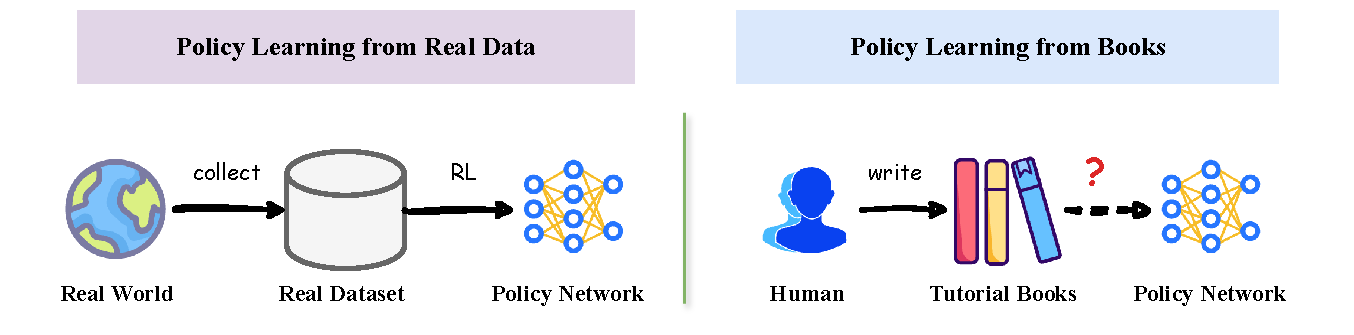
\includegraphics[width=1.0\linewidth]{fig/PER-problem.pdf}
    \caption{Comparison of the workflow of policy learning from books compared with learning from data.}
    \label{fig:problem}
    \vspace{-2mm}
\end{figure}

Humans can acquire new skills through various written materials which provide condensed knowledge, without the need of direct interactions with the target environment. 
In contrast, traditional policy learning paradigms, such as reinforcement learning (RL)~\citep{rl@2018sutton} primarily relies on trial and error~\citep{dqn2016van, ppo2017schulman, fusion2022jonas}. 
Despite recent advances in offline RL~\citep{cql@2020aviral,mopo@2020tianhe} showing that policy improvements can be achieved simply by using pre-collected data, the data collection process of the dataset can still be costly and sometimes impossible. Therefore, a question arises: similar to how humans learn, can a policy learn from books?



We argue that the recent successes of Large Language Models (LLMs) in utilizing textual data, such as GPT-4~\citep{gpt42023achiam}, and LLaMA~\citep{llama2023hugo} already demonstrated the potential to learn from textual content. However, current studies focus mainly on using LLM directly for decision making~\citep{voyager2023guanzhi, szot2023large} or integrating them as supplementary modules in other machine learning workflows~\cite{xi2023rise, hu2024survey, guo2024large}.
In this study, we introduce a novel topic built upon the shoulders of LLMs' systems: Policy Learning from Books (\topic). \topic~aims to derive a policy network directly from natural language texts, bypassing the need for numerous real-world interaction data, as shown in Figure.~\ref{fig:problem}. \textit{This can be viewed as a further step towards enabling more resources for policy learning and also a more generalized form of offline RL, which uses textbooks to learn a policy offline.} 
The essential challenge of \topic~comes from the inevitable large modality gaps between the text space, which includes the knowledge related to decision-making, and the policy network space, which formulates the parameters of the policy function. 


\begin{figure*}[h]
    \centering
    % \vspace{-5mm}
    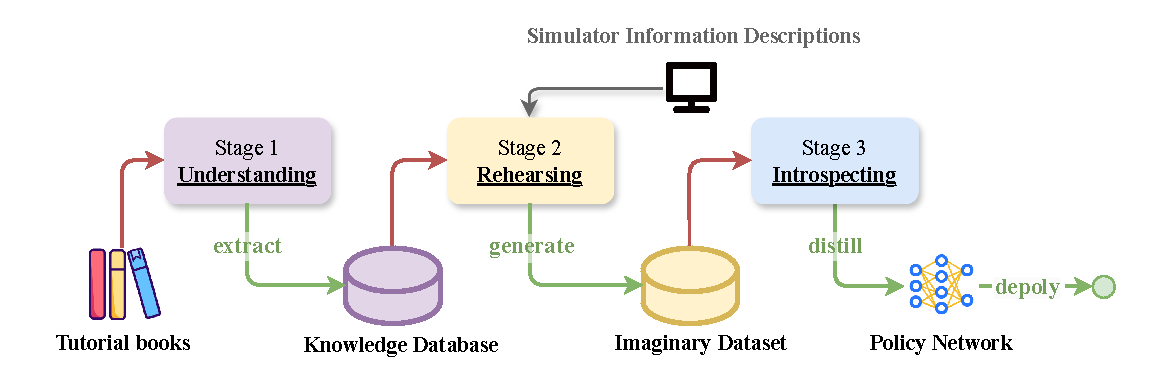
\includegraphics[width=\linewidth]{fig/framework_new.drawio (1).pdf}
    \caption{The Illustration of the understanding, rehearsal and introspection pipeline for \topic.}
    % \vspace{-2mm}
    \label{fig:framework}
\end{figure*}

To realize~\topic, inspired by human learning processes, we propose a three-stage learning methodology: understanding, rehearsal, and introspection (\algo), which is shown in Figure.~\ref{fig:framework}.  
For understanding, it first extracts knowledge from books to form a knowledge database; then it rehearses imaginary decision-making trajectories with the help of the knowledge retrieved from the database; finally, it introspects on the imaginary dataset to distill a policy network for decision-making.
We present the first practical implementation of \algo, employing LLMs to convert book paragraphs into pseudocode for policy, dynamics, and reward functions. 
This pseudocode forms a code-based knowledge database, which is used to generate an imaginary dataset based on retrieval augmented generation techniques~\citep{rag@2020patick}. A policy learning technique inspired by offline RL~\citep{mopo@2020tianhe} is then applied to distill a policy network that addresses inaccuracies in the imagined actions, rewards, and states.


% Based on the framework, we give a practical implementation for \topic: 
% It utilizes LLMs to translate paragraphs in books to pseudocode of policy function, dynamics function, and reward function respectively and form a code-based knowledge database, then generate an imaginary dataset by interactively querying an imaginary policy function, dynamics function, and reward function, which are constructed via retrieval augmented generation techniques~\citep{} with the code-based knowledge database. Finally, it uses an offline-RL-style technique for self-improving a policy network, which handles the imprecision of action, rewards, and states of the imaginary dataset together.

In the experiment, we build a testbed based on football tasks, which is popular in recent studies~\citep{football-deepmind} as a difficult decision-making task, and focus on policy learning from football tutorial books, which naturally contain condensed knowledge, especially information closely related to football skill acquisition, the environment and dynamics of football games, and ways to evaluate football behaviours. 
We collect football tutorial books from RedPajama~\citep{redpajama@2023together} and test our solution in the Google Football simulator~\citep{football2019karol}. The policy is deployed in a football game directly. Our agent controlled by the policy network could beat the built-in AI with a 37\% winning rate on average while using GPT as the football agent can only achieve a 6\% winning rate.

% The contribution of this paper can be summarized into the following three-folds. Firstly, We introduce Policy Learning from Books (\topic), a novel research idea in reinforcement learning that utilizes natural-language texts for policy learning, moving beyond the traditional reliance on real-world interaction data. Secondly, We establish a three-stage framework of \topic which mirrors human learning processes: Understanding, Rehearsing, and Introspecting (URI). URI framework represents a practical methodology of how policy can be distilled from text materials. Thirdly, we present the first practical implementation of \algo~for knowledge extraction, trajectory rehearsing, and policy distilling, based on recent advancements of LLMs, RAG, and offlineRL; We build a testbed on the football game and demonstrate the practical effectiveness and applicability of the \algo~implementation.

 %Introduction of the novel Policy Learning via Reading (\topic) approach, which uses natural-language texts for policy learning, marking a significant shift from traditional RL methods that rely heavily on real-world interaction data.


\vspace{-1mm}
\section{Related Work}
\vspace{-2mm}
% In this section, we review the close-related topics, \emph{i.e.}, Large Language Models, Retrieval Augmented Generation and Offline RL.

% \vspace{-3mm}

% \subsection{Large Language Models for Decision-Makings}
% LLM用来输出策略的几种方式:(1)直接出策略(Language-based Decision-Makings:LLM-agent),下面的全是;(2)Language-model-assistant Decision-Makings:用LLM出目标,策略,reward,guide策略探索,加速策略学习,like:RLAdapter: Bridging Large Language Models to Reinforcement Learning in Open Worlds;(3)Language-guided Decision-Makings:让策略condition on language,让策略根据人类的instruction完成不同的行为,是一种goal condition的policy。
% 我觉得区别直接讲,我们的方法是独立于上面的所有范式的新的范式,Language-derived Decision-Makings。我们直接基于语言learn一个策略出来。不用纠结于那些细节。

% \textbf{Large Language Models (LLMs).} 
LLMs have demonstrated remarkable potential in achieving human-level ability in various tasks, sparking a surge in studies investigating LLM-based autonomous agents. Based on the different roles of LLM in the agents, there are two types of work.  
% LLM can be used as a module to improve existing or be used as an actionable agent directly~\citep{voyager2023guanzhi}. Early works prefer open-loop plans and hard-code search algorithms to improve the long-term planning ability of LLM. Chain of Thought~\citep{cot2022jason} proposes inputting reasoning steps for solving complex problems into the prompt. Closed-loop planning leverages environmental feedback, thereby facilitating more adaptive decision-making. 
%  ReAct~\citep{react@2022shunyu} and Inner Monologue~\citep{inner@2022wenlong} allow
% LLM agents take single-step actions according to the environmental feedback. Reflexion~\citep{reflexion@2023noah}, further allows ReAct agent to revise itself from past trials and errors.
Firstly, LLM can be used 
% as a module to accelerate and improve existing planning/RL methods or 
as an actionable agent directly~\citep{voyager2023guanzhi}. Early works~\citep{cot2022jason, llm-mcts2023zirui} prefer open-loop plans and hard-code search algorithms to improve the long-term planning ability of LLM. Closed-loop planning~\citep{react@2022shunyu, inner@2022wenlong, reflexion@2023noah} leverages environmental feedback, thereby facilitating more adaptive decision-making. 
%  ReAct~\citep{react@2022shunyu} and Inner Monologue~\citep{inner@2022wenlong} allow
% LLM agents take single-step actions according to the environmental feedback. Reflexion~\citep{reflexion@2023noah}, further allows ReAct agent to revise itself from past trials and errors.
Secondly, LLM can be used to assist or accelerate the learning of agents. The form of assistance can be quite diverse. It can generate high-level plans~\citep{liu2023llm+, llmplanner@2023song}, rewards~\citep{drlc@2024cao, kwon2023reward, wu2024read}, transitions~\citep{zala2024envgen, ren2024bases}, or as an adapter to convert human instructions into structured inputs~\citep{hu2023instructrl}. In our work, LLMs play a different role compared to all the above-mentioned types. LLMs are to understand the knowledge in the books, rehearsing the decision-making process to derive an imaginary dataset based on the knowledge.  The policy to execute is a neural network distilled from the imaginary data without interactions with the real environments. 




\vspace{-1mm}
\section{Preliminaries}
\vspace{-2mm}

\textbf{Markov Decision Making Process (MDP)} is defined as a tuple of $\gM:=(\gS, \gA, \transf, \rewf, \gamma, \rho_0)$~\citep{rl@2018sutton} of the target environment, where $\gS$ is state space, $\gA$ is action space, $\transf:\gS\times \gA\to \Delta(\gS)$ is the transition function ($\Delta(\cdot)$ is the probability simplex), $\rewf:\gS\times \gA\to [0, R_{\max} ]$ is the reward function, $\gamma\in [0,1)$ is the discount factor, and $\rho_0$ is the initial distribution over states. A policy $\pi:\gS\to \Delta(\gA)$ describes the distribution of actions for each state. 

\textbf{Retrieval Augmented Generation (RAG)}~\citep{rag@2020patick} has shown great ability to improve LLM's generation ability for knowledge-intensive tasks. LLMs can query external data sources to obtain relevant information before proceeding to answer questions or generate text. Formally, given an LLM $\llm$, the retrieval module $\ret(x, \{y_i\})$ takes a textual query $x$ as input, finds the most relevant textual segment $y^*$ by finding the most similar $\emb(y)$ from the knowledge database $y \in \{y_i\}$ compared to $\emb(x)$. Augmentation transforms the content into an additional input for the LLM's generation. 
In this paper, RAG is used to implement the~\algo~algorithm. We use standard RAG techniques as the retrieval module, i.e., cosine similarity matching~\citep{colbert@2022khattab, kamalloo2023evaluating}, within the implementation of \algo. In particular, we use GPT embedding to index the texts in the database and also the current query, then use cosine similarity to find the top-$n$ matching data for downstream tasks, i.e., $\llm(x,[y^*_1, ..., y^*_{n}])$.

% 我感觉这里就直接分两类介绍,offlineRL有model-free和model-basd的,modelfree从数据直接学,通过考虑Q的不置信度来得到一个鲁棒策略;(2)model-based从数据学model,策略从model直接学,要考虑transition的不置信来得到一个鲁棒的策略。具体技术实现的差异不用展开。
% commentV2: 我觉得这里面的技术还是不需要展开的,我们就介绍
% 1. offlienRL的挑战是什么:OOD数据下如何做improvement
% 2. model-free的框架怎么解;
% 3. model-based的框架怎么解。
% 我们的方法把知识转化成了imaginary data,我们用它做基于RL的policy的self-improve。imaginary data 下的RL和offline data的RL的相同点在于,我们都需要考虑OOD问题。但是imaginary data 需要额外考虑由语言想象出来的数据本身的不准确的问题。


\textbf{Offline RL}~\citep{levine2020offline} addresses the problem of learning policies from a pre-collected dataset $\mathcal{D}$. 
Existing studies can be classified into two categories: model-free and model-based methods. Model-free~\citep{cql@2020aviral, brac@2019yifan, td3-bc@2021fujimoto, bear@aviral2019, rem@2020rishabh, iql@2021kostrikov, dsconstraint@2023ran} methods learn a policy directly from the dataset $\mathcal{D}$ through a special designed conservative policy learning loss which usually aims to avoid policy taking actions unseen in $\mathcal{D}$. Model-based offline algorithms~\citep{mopo@2020tianhe, morel@2022rahul, maple@2023xionghui, mobile@sun2023, genoffline@luo2024,ruifeng@icml24,pcm,galileo} first estimate the dynamics and reward model $\hat \transf$ and $\hat \rewf$ from the dataset $\mathcal{D}$. The policy is learned by iterating with $\hat \transf$ and $\hat \rewf$. In the process, specially designed penalties $\mathcal{R}$ are adopted to discourage the policy from visiting states where the model predictions are of high uncertainty.


\vspace{-1mm}
\section{Problem Formulation of Policy Learning from Books}
\vspace{-2mm}


The goal of Policy Learning from Books ({\topic}) is to use an algorithm $\rm{ALG}$ to learn a policy $\hat \pi^*=\rm{ALG}(\books, |\gM|)$ from textual books $\books$, which can maximize the cumulative discounted reward $\eta(\pi)=\sum_t\E_{a_t\sim \pi}\gamma^t\rewf(s_t,a_t)$, where the book is defined as $N_b$ segments $b_i$ divided by paragraphs, i.e., $\books:=\{b_1, ..., b_i, ..., b_{N_b}\}$, and $|\gM|$ denotes the brief textual descriptions of the structures of MDP, including the descriptions of state space, action space, the task we faced, and the initial state distribution. $|\gM|$  is inevitable to be used since $\books$ only gives general knowledge of the target environment while $|\gM|$ defines the specific information, e.g., the exact format to interact with the simulator.
% In other words, we would like to find an algorithm $\rm{ALG}$ that can minimize the value gap of $\eta(\pi^*)-\eta(\rm{ALG}(books))$, where $\pi^*$ is the optimal policy. 
Unlike standard RL, during the learning process of {\topic}, the algorithm has no access to the environment. To ensure the feasibility of extracting a non-trivial policy, we make a mild assumption that $\books$ contains the descriptions of transition functions $\{\hat \transf\}$, and reward functions $\{\hat \rewf\}$ that can be regarded as the approximations of $\transf$ and $\rewf$, respectively. It also contains descriptions of relatively high-quality behaviour policies. 



% In our work, to achieve introspection from data generated by LLMs, we build our policy distillation algorithm based on several existing techniques in offline RL, including the uncertainty penalty in Model-based Offline Policy Optimization (MOPO)~\citep{mopo@2020tianhe}, which constructs a pessimistic model that discourages the policy from visiting states where the model is inaccurate; and a model-free method, Conservative Q-learning~\citep{cql@2020aviral} to obtain a robust value function that does not overestimate unseen state-action pairs too much.

 % in offline RL for self-improvement from the data generated by the LLM. 

% Offline RL addresses the problem of learning policies from
%  a pre-collected dataset. Most methods can be classified into two categories:
%  model-free and model-based methods. Model-free methods learn a conservative policy
%   directly from the dataset. BRAC~\citep{brac@2019yifan} and TD3-BC~\citep{td3-bc@2021fujimoto} regularize the learned policy to be close to the behavior policy. BEAR~\citep{bear@aviral2019}, REM~\citep{rem@2020rishabh}, CQL~\citep{cql@2020aviral}, and IQL~\citep{iql@2021kostrikov} obtain a robust value function that does not overestimate unseen state-action pairs too much. Model-based offline
%  algorithms first estimate a model from the dataset and perform policy learning or planning based on this learned model. MOPO~\citep{mopo@2020tianhe} and MOReL~\citep{morel@2022rahul}
%  constructs a pessimistic model that discourages the policy from visiting states where the model is inaccurate. MAPLE~\citep{maple@2023xionghui} takes a slightly different way by learning a set of diverse models and requires the policy to generalize over them. 
%  In our work, we adopt the technique in offline RL for self-improvement from the data generated by the LLM. 

 % Specifically, we choose CQL~\citep{cql@2020aviral} as the base algorithm because it is simple to implement and proves robust in many tasks. We also adopt an ensemble-based uncertainty estimation, as used in many offline RL methods, to quantify the possible inaccuracy of the transition and reward. \textcolor{blue}{Interestingly, LLM outputting the transition and reward could also be seen as an implicit model, which suggests other techniques in model-based RL could also further improve the performance.}





% \section{Policy Learning from Books}

% \section{Problem Formulation of Policy Learning from Books}

% MDP definition.
% books notation. an assumption that the books contain \hat T, \hat R, \beta (behavior policy)
% objective: ALGO(BOOK) -> \hat \pi^*, which \min ||V(\pi^*) - V(\hat \pi^*)||

% All of the information 

% TODO: discuss the core challenge of \topic.

% 
% However, contrary to the traditional RL setting, the policy has no access to the environment or any data collected from it during training. Instead, it can access books $\mathcal{B}$, whose content includes the information of $\hat P, \hat R$, which are approximations of $P, R$ respectively, and that of a behavior policy $\hat\pi$, in the text format.

\vspace{-1mm}
\section{Understanding, Rehearsing, and Introspecting}
\vspace{-1mm}

In this section, we first present our motivation for the proposed three-stage framework in Section.~\ref{sec:framework}. After that, we explain how we implement those stages in Section.~\ref{sec:book_content_understanding}, \ref{sec:rehearsing}, and \ref{sec:introspecting} respectively.


\vspace{-1mm}
\subsection{Motivation of the Three-Stage Framework}
\label{sec:framework}
\vspace{-1mm}

As shown in Figure.~\ref{fig:framework}, the methodology to solve \topic~consists of three major stages: understanding, rehearsing, and introspecting (\algo). The motivation of these three modules can be easily understood by reviewing how humans learn from books: as humans, we first extract knowledge from books to extend our knowledge database. Then, to acquire skills,  we often rehearse the possible consequences of applying the skill in our mind, integrating knowledge from the books with our prior life knowledge. Finally, we will re-examine the steps we took in our minds and think how we could have done better until we confirm that we know how to execute in the real world. In this paper, we mimic the above three steps via the following modules: \textbf{Understanding} module takes paragraphs of books as input and forms a knowledge database organized in pseudo-code. \textbf{Rehearsing} module iteratively takes the current imagined state as input and outputs the action, next state, and reward with guidance from the database. After gathering these imagined content to form a dataset, \textbf{Introspecting} module distills a policy network, which should consider errors of generations of state, action, and rewards. 

We give the overall architecture of our implementation of \algo~in Figure.~\ref{fig:3-stage-implmentation}. The detailed description of how they realize these functionalities will be discussed in the following. 

% \vspace{-1em}
\vspace{-1mm}
\subsection{Book Content Understanding}
\label{sec:book_content_understanding}
\vspace{-2mm}


\begin{figure}[t]
    \vspace{-12mm}
    % \centering
    % \hspace{5mm}
    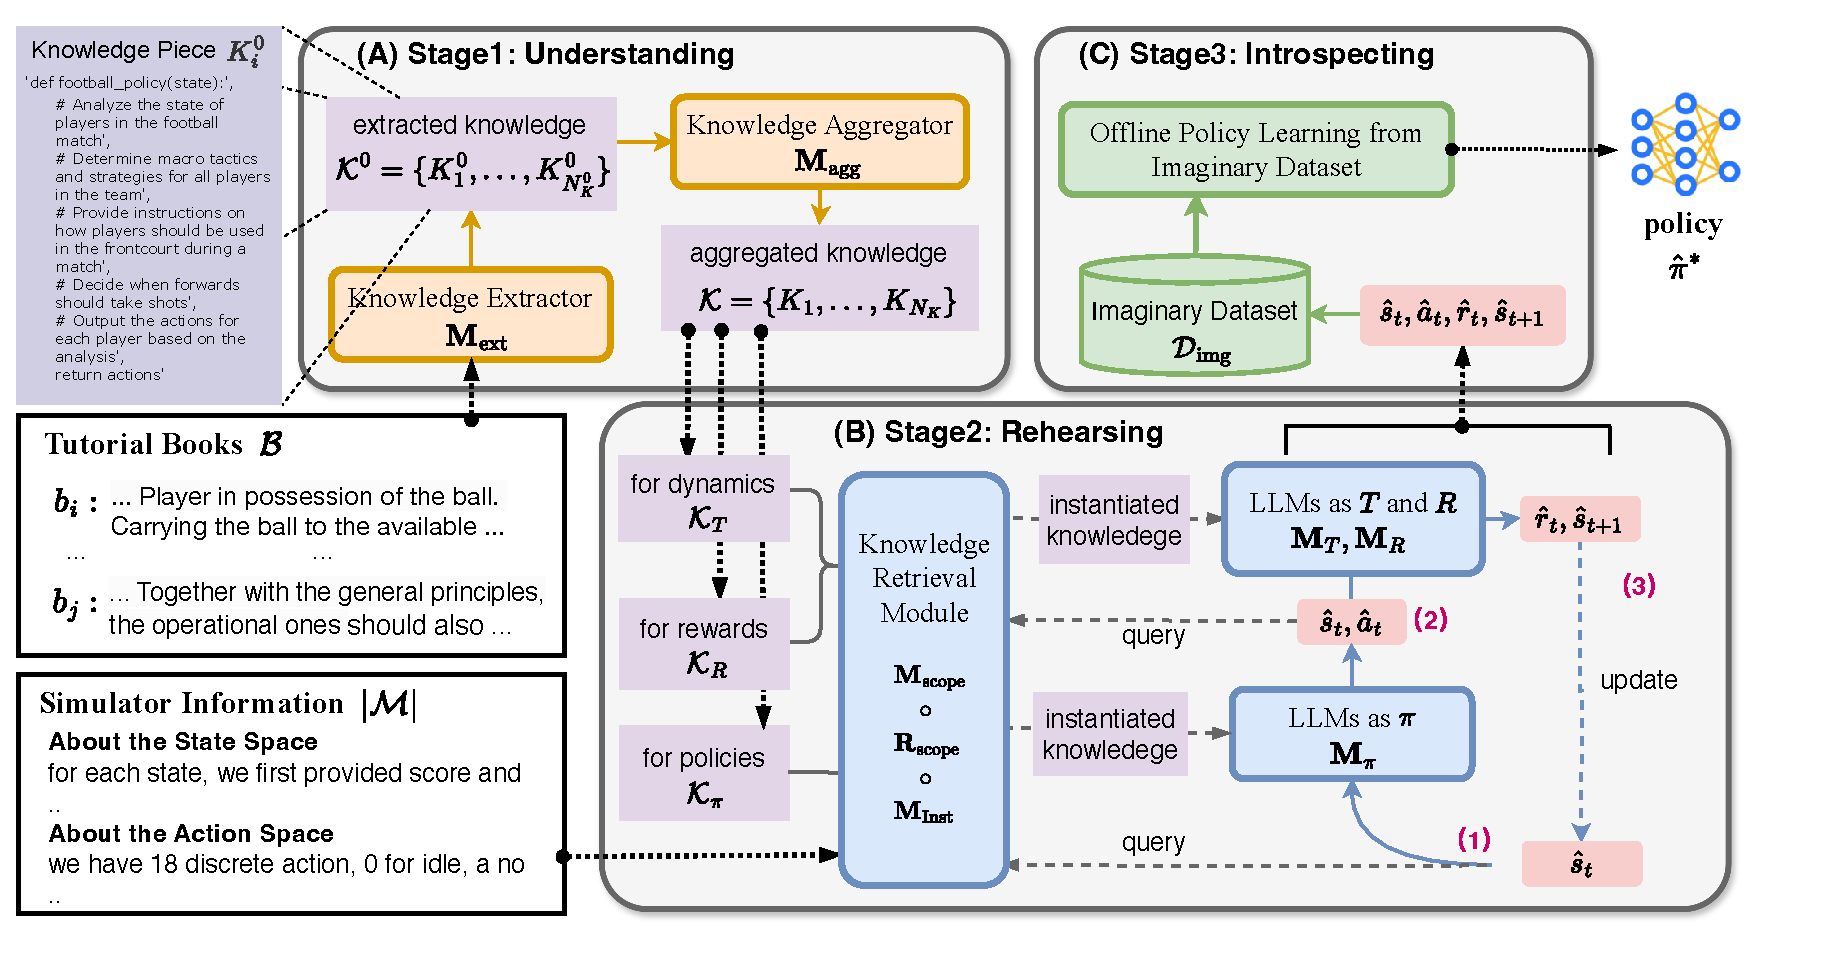
\includegraphics[width=1.06\linewidth]{fig/phrase-1.pdf}
    \vspace{-7mm}
    \caption{The URI pipeline consists of three major stages: (A) \textbf{Understanding:} The knowledge extractor and aggregator modules process paragraphs from books to form a structured knowledge database organized as pseudo-code. (B) \textbf{Rehearsing:} Using the knowledge database, the simulator generates and iterates through imagined states, actions, and rewards to create an extensive imaginary dataset. (C) \textbf{Introspecting:} The introspection module refines the policy network by evaluating and correcting errors in the generated states, actions, and rewards to ensure accurate and effective policy implementation.}
    \label{fig:3-stage-implmentation}
\vspace{-7mm}
\end{figure}

% \begin{figure}[t]
%     \vspace{-2em}
%     \centering
%     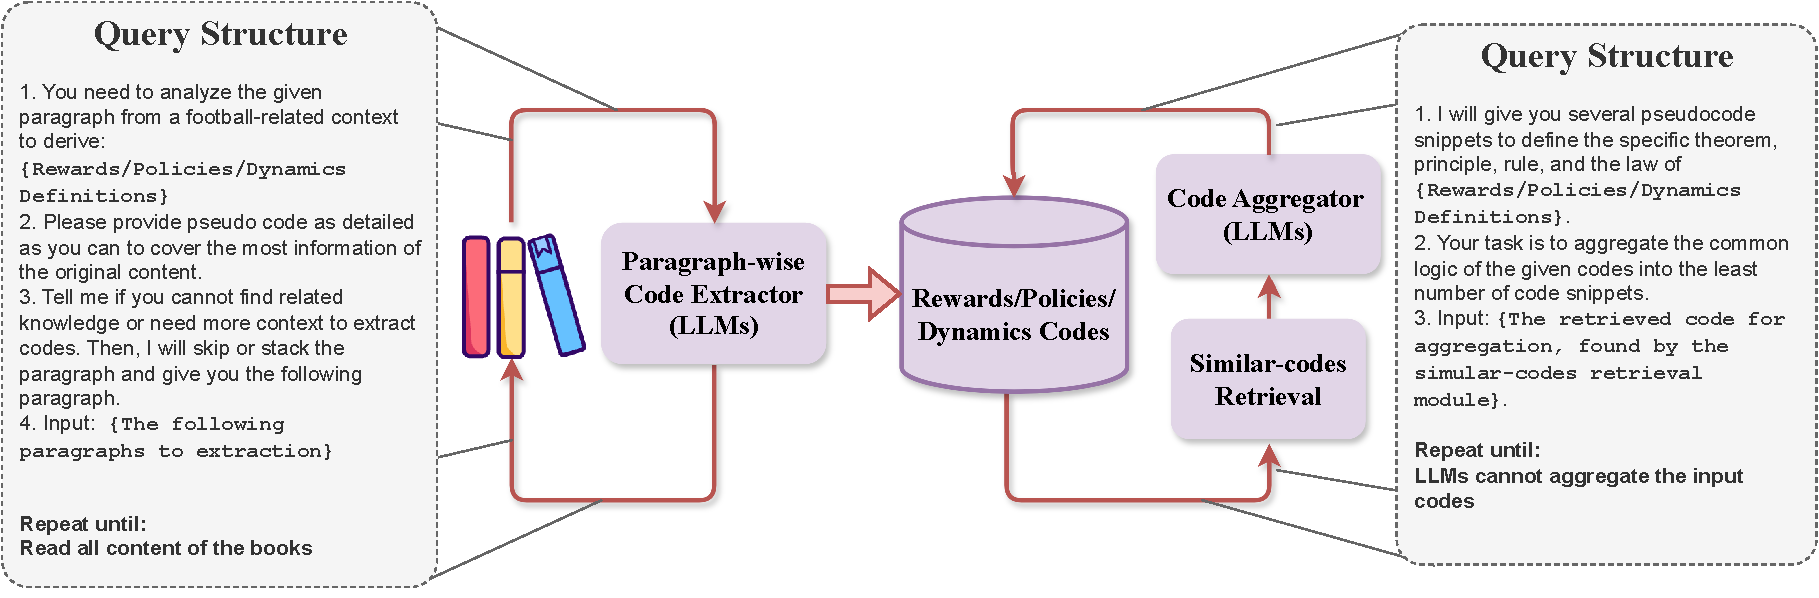
\includegraphics[width=0.2\linewidth]{fig/plb-understanding-v2 (2).pdf}
%     \caption{The procedure of understanding can be generally divided into paragraph-wise extraction (left) and iterative aggregation (right). Examples of the prompts of the two phases are also shown.  \cxh{TODO: polish this pic.}}
%     \label{fig:understanding}
% \end{figure}

% \begin{figure}[t]
%     \centering
%     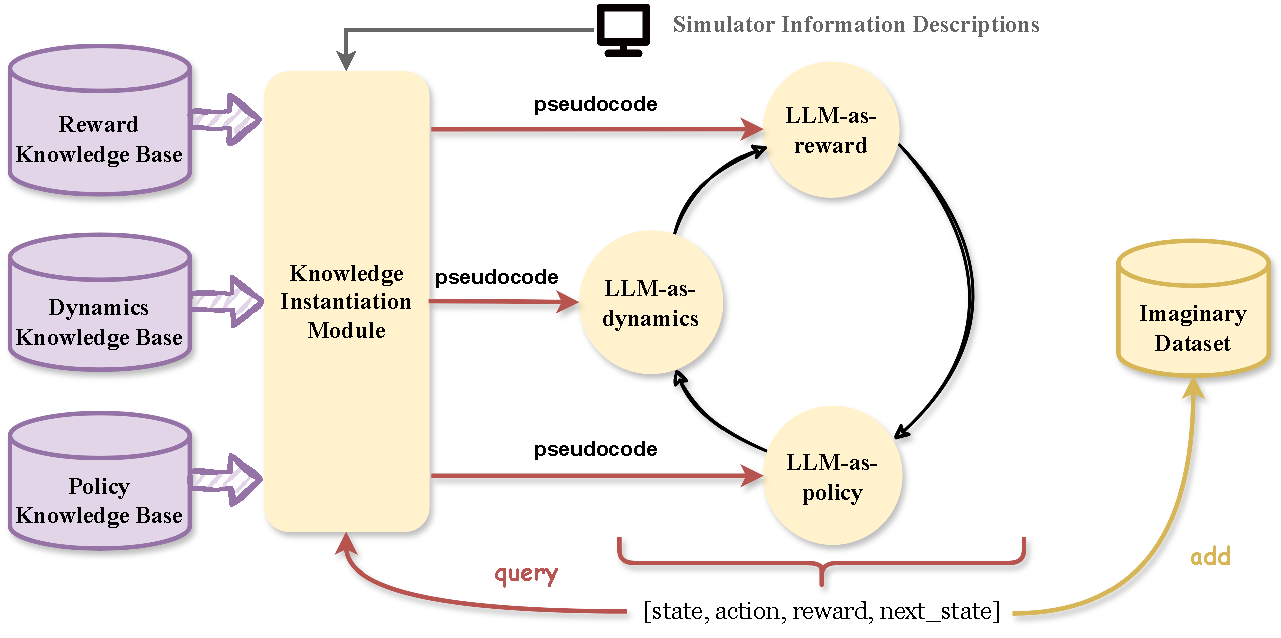
\includegraphics[width=0.2\linewidth]{fig/plfb-stage2-simp (4).pdf}
%     \caption{The procedure of retrieval relies on the code-based knowledge extracted in the understanding module (purple parts) to generate related policy, dynamics, and reward. All the generated data are stored in the imaginary dataset.
%     \yali{the figure is not clear to me. The query is given, but what's the output of this workflow? what is "simulator information description"?}}
%     \label{fig:retrieval}
% \vspace{-0.6cm}
% \end{figure}

The understanding module is responsible for extracting knowledge $\know:=\{K_1, ..., K_i, ..., K_{N_{K}}\}$ from the books $\books$, where $K_i$ denotes one piece of knowledge. For we humans, the knowledge is naturally stored in our brains. For machines, the first question is what should be the appropriate format to represent the knowledge. Since LLM has shown superior performance in code generation and codes themselves as interpretable, compact and expressive languages~\citep{llm-code2024ke}, we also choose it as the basic format of knowledge representation. Different from previous works~\citep{voyager2023guanzhi} which directly asked for runnable code for the downstream tasks using, we do not execute this code. Instead, we just use it as a more flexible and abstract description of the skill and transition while still maintaining a rigorous control flow.  As shown in Figure.~\ref{fig:3-stage-implmentation}(A), a knowledge extractor module is used as the first step. The knowledge extractor is an LLM-injected model. We iteratively ask $K_j=\llm_{\rm ext}(b_i)$ to examine whether a paragraph is related to the decision-making elements, i.e., policy functions, reward functions, dynamics functions, and how to represent them as pseudocode. 

% Books are usually long texts, possibly several hundred pages, and some of the contents are transitive words that are not directly related to skills, environment transition, and evaluations. 

Moreover, humans often learn by repeatedly reading the texts across pages and even books, by updating existing knowledge with newly learned ones and summarizing them into more general and abstract forms. A similar procedure is achieved by the knowledge aggregator module, shown in Figure.~\ref{fig:3-stage-implmentation}(A), as the second step of understanding. The knowledge aggregator is also an LLM-injected model. We iteratively ask $\llm_{\rm agg}([K_i, K_j, K_l, ...])$ to aggregate relevant knowledge among different segments based on a similarity estimation of the embedding model $\emb$. Formally, let $\know^0:=\{K_1^0, ..., K^0_{N_K^0}\}$ be the paragraph-wise knowledge extracted by $\llm_{\rm ext}$. For the $j$-the iteration, $[K^{j+1}_o, K^{j+1}_p, ...]=\llm_{\rm agg}([K^{j}_i, K^{j}_l, K^{j}_n, ...])$, where $[K^{j}_i, K^{j}_l, K^{j}_m, ...]$ is from $\know^j$ by selecting the most similar $N_{\rm agg}$ pieces of knowledge by comparing their cosine similarity under the embedding model $\emb(K)$ of GPT and $o,p,i,l,n$ here denote the indexes. $[K^{j+1}_o, K^{j+1}_p, ...]$ are then added to $\know^{j+1}$. 
% Formally, we denote the extract knowledge of the Knowledge Extractor
% The first step to understanding the contents is to identify where are the useful content, and 
% then an iterative aggregation of relevant paragraph-wise knowledge based on a similarity estimation will be adopted. 
The iteration will stop if $|\know^{j+1}|>=|\know^{j}|$, where $|\know^{j}|$ is the pieces of knowledge at $j$-th iteration. 
After iteration stops, the remaining knowledge pieces constitute the knowledge databases by splitting them into dynamics-related knowledge $\know_{\transf}$, reward-related knowledge $\know_{\rewf}$, and policy-related knowledge $\know_{\pi}$ for later modules to use. More details are provided in Appendix~\ref{app:understand}. 

% \cxh{We need A paragraph to summarize the output of the section.}
% Thanks to pseudo-codes themselves that they usually contain some descriptive words about their intent and algorithm, we use the embedding of them directly as its "key" for later retrieval rather than generating another separate annotation paragraph. 
% \textcolor{red}{We did not attempt to read the full book instantly since the summarizing done in this manner is less controllable, and the API is more expensive. }



% imaginary experience replay
\vspace{-1mm}
\subsection{Knowledge-based Rehearsing of Decision-Making}
\label{sec:rehearsing}
\vspace{-2mm}

% this section provides how we code -> data.
When humans develop a rough understanding of a new skill $\pi$ from knowledge $\know$, they will usually imagine what choice they will make given certain situations and what are the possible consequences in their minds. This rehearsing procedure would help humans correct apparent mistakes and consider better actions for long-term benefits~\citep{rehearsing@2024jia}. 


% Previous works, though encoding a search process in planning~\citep{tot2023shunyu, llm-mcts2023zirui}, or using multi-level planning to improve long-term LLM, still fail to form a closed-loop rehearsing without interaction with the environment. 
% While in \topic, we would like the LLM to generate not only the action but also the transition and the reward. 
% This full generation has two benefits: (1) it maximizes the use of knowledge in LLM acquired during the pre-training and extracted from the book; (2) it allows more flexibility in retrospecting the imagination. 
% The framework of \topic-retrieval is in Figure.~\ref{fig:retrieval}.
 
% \subsection{\mf{Imagined Data Generation}}
%{Imaginary Data Generation via Interactive Retrieval from Books}


We implement a closed-loop generation process involving the LLM-injected dynamics function $\llm_{\transf}$, reward function $\llm_{\rewf}$, and policy $\llm_{\pi}$, as depicted in Figure.~\ref{fig:3-stage-implmentation}(B). 
This approach resembles the model rollout in traditional model-based RL, where the policy, reward function, and dynamics function are represented by LLMs. Given the current imagined state $\hat s_t$, the LLMs $\llm_{\pi}$ first predict the most plausible action $\hat a_t$. Subsequently, $\llm_{\transf}$ and $\llm_{\rewf}$ generate the next state $\hat s_{t+1}$ and the associated reward $\hat r_{t}$ based on this action and the current state. In the process, a knowledge retrieval module is involved to select relevant knowledge pieces enhancing the LLM input with this information for LLM's predictions, e.g., $\hat a_{t}=\llm_{\pi}(\hat s_t, \ret(s_t, \know_{\pi}))$, $\hat r_t = \llm_{\rewf}(\hat s_t, \hat a_t, \ret(s_t, \know_{\rewf}))$ and $\hat s_{t+1} = \llm_{\transf}(\hat s_t, \hat a_t, \ret(s_t, \know_{\transf}))$. The knowledge retrieval module includes the following two steps:

\textbf{State-based Knowledge Scope Retrieval:}\label{sec:sbksr} 
% During data generation by LLMs, for each state, we initially retrieve the most relevant knowledge from our database, enhancing the LLM input with this information. 
% However, 
% Standard RAG techniques, i.e., embedding-vector similarity matching, do not work in this scenario. 
The fundamental problem of standard RAG techniques, i.e., embedding-vector similarity matching, in this scenario, is the modality gap between the query $s_t$ and the knowledge $\know$.
% Unlike standard RAG techniques, which rely on embedding-vector similarity matching, we confront a fundamental challenge due to the modality gap between the queries and the database contents. 
Standard RAG approaches aim to identify information closely related to the query, while here we need to ask the most suitable knowledge to be applied as a dynamics/reward/policy function \textit{that has the best predictions} for the queried state and action. Standard RAG techniques tend to retrieve knowledge pieces that include similar text patterns as the queried states and fail to find the best knowledge for predictions. To address this, we propose a knowledge scope retrieval method that includes a simple yet effective preprocessing step to bridge the modality gap. In particular, we traverse all knowledge pieces $K_i \in \know$ by iteratively sampling $n_{\rm scope}$ knowledge pieces $\{K_i\}_{n_{\rm scope}}$ from the database $\know$, combining them with simulator information $|\gM|$ and using LLM $\{K^S_i\}_{n_{\rm scope}}=\llm_{\rm scope}(\{K_i\}_{n_{\rm scope}},|\gM|)$ to determine the preferred scopes $K^S_i$ for each piece of knowledge. 
$K^S_i$ is defined by the preferred subspace of state to use the knowledge. Then a standard RAG technique is applied to identify the most relevant knowledge scope $K^s_j$ and its relevant knowledge $K_j$. Formally, $(\{K_j\}, \{K^S_j\})=\ret_{\rm scope}(\hat s, \know^{S})$, where $\know^{S}$ is the scopes of the knowledge database. This method is effective for embedding models in retrieving the correct knowledge as the texts of keys and queries both are about the descriptions of states. 
% one sentence summary about why  this work.

% concatenate with simulator information descriptions, e.g., the state space and action space of the football game simulator, ask LLMs for the preferred state scopes of each piece of sampled knowledge to serve as prior knowledge of rewards/dynamics/policy in the football game. Then, standard RAG techniques are applied by regarding the current state as the ``query'' and the preferred state scope as the ``key'' to find the relevant knowledge.


% When the LLMs generates data, for each state, we first need to retrieve the most relevant knowledge from the knowledge database and extend the input with the retrieved knowledge for LLMs. However, standard RAG techniques, i.e., embedding-vector similarity matching, do not work in this scenario. The fundamental problem is the modality gap between the query and the information in the database. The standard RAG techniques pursue finding the most relevant information between the query and the item in the database, while here we need to ask for the most suitable knowledge to be applied as a dynamics/reward/policy function in the queried state and action \textit{for the best predictions}. Standard RAG techniques will just tend to retrieve the knowledge that includes similar meanings as the queried states and fail to find the best knowledge for predictions. 

% In this article, we propose a simple yet effective retrieval method, which includes a prepossess step to bridge the modality gap. 
% In particular, we iterate choose $n_{\rm scope}$ pieces of code-based knowledge from the database, concatenate with simulator information descriptions, e.g., the state space and action space of the football game simulator, ask LLMs for the preferred state scopes of each piece of sampled knowledge to serve as prior knowledge of rewards/dynamics/policy in the football game. Then, standard RAG techniques are applied by regarding the current state as the ``query'' and the preferred state scope as the ``key'' to find the relevant knowledge.

\textbf{Post-Retrieval: Knowledge Instantiation:} Predicting based on code knowledge requires the LLM's robust understanding of code.  We refine this process employing an LLM to instantiate the code $K^I=\llm_{\rm Inst}(\hat s, |\mathcal{M}|, \{K_j\})$ based on the current state $\hat s$, the simulator information description $|\mathcal{M}|$ and the knowledge $\{K_j\}$ retrieved by $\ret_{\rm scope}$.
Knowledge instantiation involves generating a specific pseudocode based on the football-related knowledge coded in the retrieved information, tailored to the simulator's current state and action requirements. 
% In this way, the instantiated pseudocode conforms to the simulator's design, suggesting actions, rewards, or subsequent states based on the observed information. 

Finally, three LLMs are involved to generate the imaginary dataset $\mathcal{D}_{\rm img}$, including $\hat a_{t}=\llm_{\pi}(\hat s_t, \llm_{\rm Inst}(s_t, |\mathcal{M}|, \ret_{\rm scope}({\hat s}, \know_{\pi}^S)))$, $\hat r_{t}=\llm_{\rewf}(\hat s_t, \hat a_t, \llm_{\rm Inst}(s_t, |\mathcal{M}|, \ret_{\rm scope}({\hat s}, \know_{\rewf}^S)))$ and~$\hat s_{t+1}=\llm_{\transf}(\hat s_t, \hat a_{t}, \llm_{\rm Inst}(s_t, |\mathcal{M}|, \ret_{\rm scope}({\hat s}, \know_{\transf}^S)))$, where $\know_{\pi}^S$, $\know_{\rewf}^S$, and $\know_{\transf}^S$ are the scope of the knowledge database $\know_{\pi}$, $\know_{\rewf}$, and $\know_{\transf}$ respectively. To start the rollout of a trajectory, we need a state as the initial state. It has several choices to achieve, e.g., sampled from $\gS$, generated by another LLM, or pre-collected a small number of real states from the target environments as part of simulator information. Since the first two choices might involve more unrealistic initial states, to simplify the difficulty of the task, we pre-collected a small number of real states in this article. The detailed setup is in the experiment section. Besides, during the rollout over $H$ steps, we reuse instantiated knowledge to reduce the overload of LLM's callings. More details are provided in Appendix~\ref{app:rehearsing}.
% This approach offers two advantages: it reduces the number of calls to the more powerful LLM, thus lowering calling costs, and it explicitly translates general football knowledge into specific knowledge relevant to the current simulator state, enhancing the LLM's effectiveness in downstream tasks. 
  
% 基于代码知识做出对应的决策需要依赖于更大规模的LLMs,实现对代码的强理解。而大的语言模型(比如GPT4)意味着较高的调用成本。为了生成大量数据,我们需要反复的调用LLM,这意味着较大的成本开销。本文对这个问题做了一个优化。具体而言,我们使用较强的LLM (GPT-4) 来根据当前的状态,动作信息,simulator information description,和Retrieved Knowledge实例化代码。实例化指的是,根据retrieved得到的基于代码表示的对于football本身的knowledge,根据当前的simulator的information,和具体面临的state和action给出更具体的伪代码,他根据状态空间提供的观测信息给出符合模拟器设计规范的对应的动作,奖励值,或者下一步的状态。之后,在rollout的$n_{\rm repest}$步过程中,我们会复用这个实例化的代码,使用较弱的语言模型来实现reward,dynamics和policy的功能。这么做有两个好处,(1)减小了调用了强语言模型的次数,降低了开销;(2)实例化的过程中把general的football相关的knowledge transfer成了根据当前的simulator和具体面临的state相关的具体的knowledge。

% adopt the retrieval-augmented generation technique. When the LLM generates the data, it first retrieves the most relevant knowledge from the database collected in the previous stage and extends the input with the retrieved knowledge. The relevance is measured by the embedding lookup based on the current state. A two-level generation implements the rehearsing. The higher level is responsible for outputting general and long-term instructions about the game whose inputs are merely the current state. The lower level, given the strategy generated by the higher level, is specialized to output environment-related actions. This two-level generation also promotes the reuse of the general knowledge across tasks of a similar field: only the low-level environment-specific generation needs to adapt.



% \begin{figure*}
%     \centering
%     \includegraphics[width=0.95\linewidth]{fig/per-retrieval.pdf}
%     \caption{Illustration of the book-retrieval module and the imaginary data generator.}
%     \label{fig:retrieval}
% \end{figure*}


% \sy{some prompt and output example}
\vspace{-5mm}
\subsection{Introspecting based on the Imaginary Dataset}
\label{sec:introspecting}
\vspace{-2mm}

% \textbf{Offline RL} addresses the problem of learning policies from a pre-collected dataset~\citep{cql@2020aviral,dsconstraint@2023ran,mopo@2020tianhe,maple@2023xionghui, mobile@sun2023}. 
% Existing works can be classified into two categories: model-free and model-based methods. Model-free~\citep{brac@2019yifan, td3-bc@2021fujimoto, bear@aviral2019, rem@2020rishabh, cql@2020aviral, iql@2021kostrikov, dsconstraint@2023ran} methods learn a conservative policy directly from the dataset. 
% Model-based offline algorithms~\citep{mopo@2020tianhe, morel@2022rahul, maple@2023xionghui, mobile@sun2023, genoffline@luo2024} first estimate a model from the dataset and perform policy learning or planning based on this learned model. 
% In our work, to achieve introspection from data generated by LLMs, we build our policy distillation algorithm based on several existing techniques in offline RL, including the uncertainty penalty in Model-based Offline Policy Optimization (MOPO)~\citep{mopo@2020tianhe}, which constructs a pessimistic model that discourages the policy from visiting states where the model is inaccurate; and a model-free method, Conservative Q-learning~\citep{cql@2020aviral} to obtain a robust value function that does not overestimate unseen state-action pairs too much.

% What is X for human beings?
% What is the purpose of X in \topic?
% What is the challenge of implementing X?
% how do we handle these challenges?
% \cxh{Maybe we can follow : (1) What is X for human beings? (2)  What is the purpose of X in \topic?; (3) What is the challenge of implementing X?; (4) how do we handle these challenges? for these three subsection.}
The direct output LLM in the rehearsing stage can be sub-optimal or incorrect. We would like to re-examine the collected data and try to distill a policy that can avoid the side effects. 
% This distillation also brings practical benefits: only the small policy, instead of the LLM, is needed for the final deployment which drastically reduces the deployment cost. 
We can regard the data $\mathcal{D}_{\rm img}$ collected during the rehearsing stage as an offline dataset and apply offline RL algorithms to train an improved policy from the dataset. 
However, directly applying existing offline RL algorithms over-simplifies the problem. Compared with the standard offline setting where only the behavior policy is sub-optimal, there is an additional misalignment in the data generated during the rehearsal: the transition and the reward function estimated by the LLM are also inaccurate. Overlooking such inaccuracy would result in a policy exploiting the sub-optimal transition and reward function and cause performance degradation or even risky behaviors in the final deployment. 

To solve the problem, in this paper, we adopt the Conservative Q-learning ~\citep{cql@2020aviral} as the base offline RL algorithm, whose learning objective is as follows:
\begin{small}
$$\begin{aligned}
\min _Q \max_\pi~&\alpha\left(\mathbb{E}_{\hat s \sim \mathcal{D}_{\rm img}, a \sim \pi(a \mid \hat s)}\left[Q(\hat s, a)\right]-\mathbb{E}_{\hat s, \hat a \sim \mathcal{D}_{\rm img}}[Q(\hat s, \hat a)]+\mathcal{R}(\pi)\right)  +\mathbb{E}_{\hat s, \hat a \sim \mathcal{D}_{\rm img}}[(Q(\hat s, \hat a)-\hat{\mathcal{B}}^{\pi} \hat{Q}(\hat s, \hat a))^2],
\end{aligned}$$
\end{small}
where $\hat{\mathcal{B}}^{\pi} \hat{Q}$ is the bellman update operator to update the Q-value function~\citep{rl@2018sutton}, and the first term is to learn a policy with conservative Q value~\citep{cql@2020aviral}. As a solution of introspecting from imaginary data, as shown in Figure.~\ref{fig:3-stage-implmentation}(C), we add the uncertainty of the reward and transition estimation as the regularization terms, $\mathcal{R}_{\rewf}$ and $\mathcal{R}_{\transf}$ over the original reward $\hat r$ output by the LLM $\llm_{\rewf}$. In practice, we adopt these regularization terms by applying them when we backup the $\hat Q^k$:
\begin{align*}
    \hat{\mathcal{B}}^{\pi}_{\rm I} \hat{Q}(\hat s, \hat a) := \hat r - \eta_{\rewf} \mathcal{R}_{\rewf}(\hat s, \hat a) - \eta_{\transf} \mathcal{R}_{\transf}(\hat s, \hat a) + \gamma \mathbb{E}_{\hat s' \sim \mathcal{D}_{\rm img}, a' \sim \pi_k(a' |\hat s')}[Q(\hat s', a') ],
\end{align*}
where $\hat s' \sim \mathcal{D}_{\rm img}$ is to sample the next state given $\hat s, \hat a$, $\eta_\rewf$ and $\eta_\transf$ are two hyper-parameters to control the weighting of the uncertainty terms. Inspired by Model-based Offline Policy Optimization (MOPO)~\citep{mopo@2020tianhe}, the uncertainty is estimated by an ensemble of $N_{\rm ens}$ Gaussian models of $\hat \transf$ and $\hat \rewf$, which is learned by maximizing logarithmic likelihood from the imaginary dataset. Then the uncertainty is estimated by $\mathcal{R}_{\rewf}(s, a) = \max_{i\in\{1, \dots, N_{\rm ens}\}} \sigma^r_i(s, a)$ and $\mathcal{R}_{\transf}(s, a)=\max_{i\in\{1, \dots, N_{\rm ens}\}} \sigma^T_i(s, a)$, where $\sigma^r_i$ and $\sigma^T_i$ are the $i$-th reward and dynamics model's predicted standard deviation for $s, a$ respectively. We call the solution of CQL with $\hat{\mathcal{B}}^{\pi}_{\rm I}$ as the bellman update operator Conservative Imaginary Q-Learning (CIQL). 
This regularization is easy to implement and can force the policy to generalize better over the regions where the LLM outputs inconsistent next states and rewards.



% \clearpage

\vspace{-1mm}
\section{Experiments}
\vspace{-2mm}

This section empirically evaluates our method using the Google Research Football environment (GRF)~\citep{kurach2020google}. We first introduce the experimental settings and then conduct experiments in various difficulties of GRF 11 vs 11 scenarios to compare our method with relevant baselines.

\subsection{Experiment Setups}

\paragraph{Google Research Football}\citep{kurach2020google} is a physics-based 3D football simulator that supports the main football rules such as goals, fouls, corners, penalty kicks, and offside. Google Research Football (GRF) includes a built-in AI bot for the opposing team, whose difficulty can be adjusted between 0 and 1. We define three custom difficulty levels for our experiments on the 11vs11 scenario: easy, medium, and hard. The difficulty levels differ in the bot's reaction time and decision-making defined in GRF, with higher difficulty corresponding to a stronger opponent. The major metric in our experiment is Goal Difference per Match (GDM), calculated as the average number of goals scored in all league matches minus the average number of goals conceded per match. An illustration of the game can be seen in Figure.~\ref{fig:football_main}.  For more details about the GRF implementation, please refer to Appendix~\ref{app:grf}.




\paragraph{Datasets.} We utilize two datasets in our approach. The first is the textbook dataset, which serves as the knowledge base for the \topic~framework. We collect this dataset from the open source book dataset RedPajama-1T~\citep{together2023redpajama}, focusing on titles and abstracts related to football or soccer. After filtering, we obtain a curated set of ninety books closely aligned with the domain. The second dataset is the initial state of our imaginary data generation process. 
We sample 7,500 states from the rollout of a rule-based policy in GRF competing with the hard built-in AI. Due to limited resources, to distill the policy, we imagine 75,000 transitions via \algo, which is 10 times compared to the initial states.

% During the imaginary data generation step, we treat each sampled data point as an initial state and generate $H$ future timesteps using our proposed methodology. This seeding strategy helps ground the imaginary data and improves the overall quality of the generated trajectories.

\paragraph{Baselines.} There are three baselines involved in the experiments. \textbf{LLM-as-agent} directly uses a large language model (GPT 3.5) to output actions conditioned on the current state description. \textbf{LLM-RAG} enhances LLM-as-agent by retrieving relevant knowledge from the database extracted from the tutorial books, similar to the retrieval step in our rehearsing stage, but directly outputs the action without policy learning. \textbf{Rule-based-AI} is a rule-based policy from the Kaggle Football Competition~\citep{anvarov2020football}\footnote{\url{https://github.com/Sarvar-Anvarov/Google-Research-Football}}, which is hand-designed and serves as a reference for the performance of hand-coded policies. \textbf{Random Policy} randomly chooses actions. For the implementation details about the baselines, please refer to Appendix~\ref{app:baseline}.

% \newcolumntype{a}{>{\columncolor{Gray}}c}
\newcolumntype{b}{>{\columncolor{mywhite}}c}


\begin{table*}[t]
\centering
\vspace{-7mm}
\caption{Performance Comparison of Different Policies Against Built-in AI Levels in a GRF 11 vs 11 settings, where the performance of URI is averaged among three different seeds, LLM-as-agent, LLM-RAG is tested with 10 matches, and URI policy and random policy is tested with 40 matches.}
\resizebox{0.85\textwidth}{!}{%
\begin{tabular}{c|c|c|c|c|b||c}
\toprule
\textbf{Level} & & \textbf{LLM-as-agent} & \textbf{LLM-RAG} & \textbf{Random Policy} & \textbf{\algo~(Ours)} & \textbf{Rule-based-AI} \\
\midrule
\multirow{4}{*}{\rotatebox{90}{\textbf{Easy}}} 
& Win & 20\% & 30\% & 2\% & \textbf{37\% $\pm$ 4\%} & 70\% \\
& Draw & 60\% & 60\% & 55\% & 57\% $\pm$ 4\% & 30\% \\
& Lose & 20\% & 10\% & 43\% & 6\% $\pm$ 4\% & 0\% \\
\cmidrule(lr){2-7}
& GDM & 0.0 & 0.2 & -0.58 & \textbf{0.40 $\pm$ 0.14} & 0.7 \\
\midrule
\multirow{4}{*}{\rotatebox{90}{\textbf{Medium}}} 
& Win & 0\% & 20\% & 2\% &  \textbf{42\% $\pm$ 12\%} & 70\% \\
& Draw & 60\% & 60\% & 43\% & 50\% $\pm$ 8\% & 30\% \\
& Lose & 40\% & 20\% & 55\% & 8\% $\pm$ 4\% & 0\% \\
\cmidrule(lr){2-7}
& GDM & -0.4 & 0.0 & -0.76 & \textbf{0.43 $\pm$ 0.24} & 0.7 \\
\midrule
\multirow{4}{*}{\rotatebox{90}{\textbf{Hard}}} 
& Win & 0\% & 0\% & 3\% &  \textbf{32\% $\pm$ 14}\% & 30\% \\
& Draw & 50\% & 40\% & 43\% & 58\% $\pm$ 6\% & 70\% \\
& Lose & 50\% & 60\% & 53\% & 10\% $\pm$ 7\% & 0\% \\
\cmidrule(lr){2-7}
& GDM & -0.5 & -0.6 & -0.73 & \textbf{0.32 $\pm$ 0.14} & 0.3 \\
\midrule
\multirow{2}{*}{\textbf{Average}} & Win & 6.7\% $\pm$ 9.4\% & 16.7\% $\pm$ 12.5\% & 2.3\% $\pm$ 0.5\%& \textbf{40.3\% $\pm$ 6.2\%} & 56\% \\ & GDM & -0.30 $\pm$ 0.22 & -0.13 $\pm$ 0.34 & -0.69 $\pm$ 0.08 & \textbf{0.38 $\pm$ 0.05} & 0.56 \\
\bottomrule
\end{tabular}
}
\label{tab:main_res}
\vspace{-0.5cm}
\end{table*}





\subsection{Policy Performance Compared with Built-in AIs}

 The results in Table \ref{tab:main_res} demonstrate the superiority of the proposed URI approach compared to the baselines in the 11 vs 11 full-game scenarios of the GRF environment. The LLM-based agents, including LLM-as-agent and LLM-RAG, exhibit zero-shot task completion capabilities, outperforming the Random Policy. However, even with the use of RAG techniques, the best-performing LLM-agent can only barely match the performance of the Medium-level built-in AI and fails to achieve any wins against the Hard-level built-in AI. In contrast, URI surpasses the performance of the baseline methods on all difficulty levels. Surprisingly, in the Hard task, URI achieves a higher win rate than the Rule-based Policy. We believe this is due to URI's ability to leverage knowledge from football textbooks and generate high-quality imaginary data for policy learning, enabling it to learn more adaptable and robust policies compared to the hand-crafted Rule-based-AI. These results highlight the effectiveness of the URI in learning strong policies that can handle challenging opponent tasks.





% \begin{table*}[t]
% \centering
% \resizebox{\textwidth}{!}{%
% \begin{tabular}{c|c|c|c|c|c|c|c|c|c|c|c|c}
% \toprule
% & \multicolumn{4}{c|}{11\_vs\_11 (Easy)} & \multicolumn{4}{c|}{11\_vs\_11 (Med)} & \multicolumn{4}{c}{11\_vs\_11 (Hard)} \\
% \midrule
% Method & GDM & Win & Draw & Lose & GDM & Win & Draw & Lose & GDM & Win & Draw & Lose \\
% \midrule
% \cellcolor{mywhite}\algo~(Ours)  & \cellcolor{mywhite} \textbf{0.40 $\pm$ 0.14} & \cellcolor{mywhite} \textbf{37\% $\pm$ 4\%} &\cellcolor{mywhite} 57\% $\pm$ 4\% &\cellcolor{mywhite} 6\% $\pm$ 4\% &\cellcolor{mywhite} \textbf{0.43 $\pm$ 0.24} &\cellcolor{mywhite}42\% $\pm$ 12\% & \cellcolor{mywhite} 50\% $\pm$ 8\% & \cellcolor{mywhite} 8\% $\pm$ 4\% &\cellcolor{mywhite} \textbf{0.32 $\pm$ 0.14} & \cellcolor{mywhite} 32\% $\pm$ 14\% & \cellcolor{mywhite} 58\% $\pm$ 6\% & \cellcolor{mywhite} 10\% $\pm$ 7\% \\
% LLM-as-agent & 0.0 & 20\% & 60\% & 20\% & -0.4 & 0\% & 60\% & 40\% &-0.5 & 0\% & 50\% & 50\% \\
% LLM-RAG & 0.2 & 30\% & 60\% & 10\% &0.0  & 20\% & 60\% & 20\% & -0.6 & 0\% & 40\% & 60\% \\
% Random Policy & -0.58 & 2\% & 55\% & 43\% & -0.76 & 2\% & 43\% & 55\% &-0.73 & 3\% & 43\% & 53\% \\
% \midrule
% Rule-based-AI & 0.7 & 70\% & 30\% & 0\% & 0.7 & 70\% & 30\% & 0\% &0.3 & 30\% & 70\% & 0\% \\
% \bottomrule
% \end{tabular}
% }
% \caption{Performance Comparison of Different Policies Against Built-in AI Levels in a Football Simulator, where the performance of URI is averaged among three different seeds, LLM-as-agent, LLM-RAG is tested with 10 matches, and the random policy is tested with 60 matches.
% % In the game \textbf{11\_vs\_11}, both teams are eleven players, and the difficulties mean the opponent's skill level with the game build-in AI. For more detailed information, please refer to Appendix .\ref{}
% }
% \label{tab:main_res}
% \vspace{-0.5cm}
% \end{table*}




% \begin{table*}[t]
% \centering
% \resizebox{\textwidth}{!}{%
% \begin{tabular}{c|c|c|c|c|c|c|c|c|c|c|c|c}
% \toprule
% & \multicolumn{4}{c|}{11\_vs\_11 (Easy)} & \multicolumn{4}{c|}{11\_vs\_11 (Med)} & \multicolumn{4}{c}{11\_vs\_11 (Hard)} \\
% \midrule
% Method & GDM & Win & Draw & Lose & GDM & Win & Draw & Lose & GDM & Win & Draw & Lose \\
% \midrule
% \addlinespace
% \cellcolor{mywhite}\algo~(Ours)  & \cellcolor{mywhite} \textbf{0.40 $\pm$ 0.14} & \cellcolor{mywhite} \textbf{0.37 $\pm$ 0.04} &\cellcolor{mywhite} 0.57 $\pm$ 0.04 &\cellcolor{mywhite} 0.06 $\pm$ 0.04 &\cellcolor{mywhite} \textbf{0.43 $\pm$ 0.24} &\cellcolor{mywhite}0.42 $\pm$ 0.12 & \cellcolor{mywhite} 0.50 $\pm$ 0.08 & \cellcolor{mywhite} 0.08 $\pm$ 0.04 &\cellcolor{mywhite} \textbf{0.32 $\pm$ 0.14} & \cellcolor{mywhite} 0.32 $\pm$ 0.14 & \cellcolor{mywhite} 0.58 $\pm$ 0.06 & \cellcolor{mywhite} 0.10 $\pm$ 0.07 \\
% \addlinespace\addlinespace
% LLM-as-agent & 0.0 & 0.2 & 0.6 & 0.2 & -0.4 & 0.0 & 0.6 & 0.4 &-0.5 & 0.0 & 0.5 & 0.5 \\
% \addlinespace\addlinespace
% LLM-RAG & 0.2 & 0.3 & 0.6 & 0.1 &0.0  & 0.2 & 0.6 & 0.2 & -0.6 & 0.0 & 0.4 & 0.6 \\
% \addlinespace\addlinespace
% Random Policy & -0.58 & 0.02 & 0.55 & 0.43 & -0.76 & 0.02 & 0.43 & 0.55 &-0.73 & 0.03 & 0.43 & 0.53 \\
% \addlinespace\addlinespace
% \midrule
% \midrule
% % averaged rate\\
% % {'rew': -0.6944444444444445, 'win': 0.022222222222222223, 'draw': 0.47222222222222227, 'lose': 0.5055555555555555, 'replaced_rate': 0.2374343030572211, 'rew_11_vs_11_level_0': -0.5833333333333334, 'win_11_vs_11_level_0': 0.016666666666666666, 'draw_11_vs_11_level_0': 0.55, 'lose_11_vs_11_level_0': 0.43333333333333335, 'replaced_rate_11_vs_11_level_0': 0.23908505440817235, 'rew_11_vs_11_level_1': -0.7666666666666667, 'win_11_vs_11_level_1': 0.016666666666666666, 'draw_11_vs_11_level_1': 0.43333333333333335, 'lose_11_vs_11_level_1': 0.55, 'replaced_rate_11_vs_11_level_1': 0.22922496113701973, 'rew_11_vs_11_level_2': -0.7333333333333333, 'win_11_vs_11_level_2': 0.03333333333333333, 'draw_11_vs_11_level_2': 0.43333333333333335, 'lose_11_vs_11_level_2': 0.5333333333333333, 'replaced_rate_11_vs_11_level_2': 0.2439928936264712}
% Rule-based-AI & 0.7 & 0.7 & 0.3 & 0.0 & 0.7 & 0.7 & 0.3 & 0.0 &0.3 & 0.3 & 0.7 & 0.0 \\
% \bottomrule
% \end{tabular}
% }
% \caption{Performance Comparison of Different Policies Against Built-in AI Levels in a GFootball Simulator, where the performance of URI is averaged among three different seeds, LLM-as-agent, LLM-RAG is tested with 10 matches, and the random policy is tested with 60 matches.
% % In the game \textbf{11\_vs\_11}, both teams are eleven players, and the difficulties mean the opponent's skill level with the game build-in AI. For more detailed information, please refer to Appendix .\ref{}
% }
% \label{tab:main_res}
% \vspace{-0.5cm}
% \end{table*}

% The main result is shown in Table.\ref{tab:main_res}. 1. 首先我们看到,所有的基线的效果都优于random策略,说明基于LLM的agent是具有zero-shot的完成该任务的能力的;但是,即使是使用了RAG技术的LLM-agent,最好也只能勉强和Medium-level的builtinAI持平,在Hard难度上完全无法取胜。
% 2. 相比之下,Uri是唯一一个能够战胜所有level的AI的方法,且其GDM也显著超过了基线的最好水平,


% \begin{table*}[t]
%     \centering
%     \resizebox{\textwidth}{!}{%
%     \begin{tabular}{c|c|c|c|c|c|c|c|c|c|c|c|c|c|c|c|c}
%     \toprule
%          &  \multicolumn{4}{c|}{\algo} & \multicolumn{4}{c|}{LLM-as-agent}  & \multicolumn{4}{c|}{LLM-RAG} & \multicolumn{4}{c}{Rule-based-AI} \\
%          \midrule
%         %    & \multicolumn{3}{c|}{Mean (Mid/Left/Right)}  & \multicolumn{3}{c|}{Mean (Mid/Left/Right)}  & \multicolumn{3}{c|}{Mean (Mid/Left/Right)}  & \multicolumn{3}{c}{Mean (Mid/Left/Right)}  \\  
%         % \midrule
%          % 11\_vs\_1 (Easy)  & \multicolumn{3}{c|}{11111} & \multicolumn{3}{c|}{11111} & \multicolumn{3}{c|}{11111} & \multicolumn{3}{c}{0.53~(0.93/0.36/0.30)} \\  
%          % 11\_vs\_1 (Med)  & \multicolumn{3}{c|}{11111} & \multicolumn{3}{c|}{11111} & \multicolumn{3}{c|}{11111} & \multicolumn{3}{c}{0.41~(0.75/0.28/0.25)} \\  
%          % 11\_vs\_1 (Hard)  & \multicolumn{3}{c|}{11111} & \multicolumn{3}{c|}{11111} & \multicolumn{3}{c|}{11111} & \multicolumn{3}{c}{0.39~(0.72/0.29/0.17)} \\  
%          \midrule
%          Task & GDM & Win & Draw & Lose & GDM & Win & Draw & Lose& GDM & Win & Draw & Lose& GDM & Win & Draw & Lose\\
%          \midrule
%          11\_vs\_11 (Easy) & 0.40 $\pm$ 0.14 & 0.37 $\pm$ 0.04 & 0.57 & 0.06 & &  0.2 & 0.6 &  0.2 & &  0.3 & 0.6 & 0.1 &  & 0.7 & 0.3 & 0.0\\
%          11\_vs\_11 (Med) & 0.43 $\pm$ 0.24  & 0.42 & 0.50 & 0.08 & 0.0 & 0.6 & 0.4 & 0.2 & 0.6 & 0.2 & 0.7 & 0.3 & 0.0 \\
%          11\_vs\_11 (Hard) & 0.32 $\pm$ 0.14 & 0.32 & 0.58 & 0.10 &  0.0 & 0.5 &  0.5& 0.0 & 0.4 & 0.6 & 0.3 & 0.7 & 0.0 \\
%         \midrule
%         \midrule
%         averaged rate\\
%         \bottomrule
%     \end{tabular}
%     }
%     \caption{Performance Comparison of Different Policies Against Built-in AI Levels in a Football Simulator. GDM is an abbreviation of Goal Difference per Match, which is calculated as the average number of goals scored in all league matches minus the average number of goals conceded per match.
%     % In the game \textbf{11\_vs\_1}, our team have eleven players, and the opponent team has only one goalkeeper. It includes three types of difficulty, showing the distance from the goalkeeper from near to far. Each type of map provides attack tests from centre, left, and right, the ball will therefore appear in the corresponding direction according to the test, the test is one-time, if the goal is +1, other situations (such as not kicking in, going out of bounds, being guarded by the goalkeeper, etc.) are 0.  
%     % In the game \textbf{11\_vs\_11}, both teams are eleven players, and the difficulties mean the opponent's skill level with the game build-in AI. For more detailed information, please refer to Appendix .\ref{}
%     }
%     \label{tab:main_res}
% \end{table*}






% \begin{itemize}
%     \item discussion on results
%     \item capabilities graph [ziyan] [lp]
% \end{itemize}
% In this section, we present a comprehensive benchmark of various policy algorithms against built-in AI agents across multiple levels of complexity. The evaluation metrics include win, draw, and loss rates, offering a holistic view of each algorithm's performance. The benchmarked algorithms include Policy Learning via Reading (PER),  and traditional Rule-based AI. These were tested across five distinct levels, escalating in difficulty, to ascertain their adaptability and learning efficiency in diverse environments. An aggregated rate across all levels is provided to summarize overall performance.


% In evaluating the effectiveness of our proposed LLM-based methodologies, we conducted a series of benchmark tests against various built-in AI levels in a simulated football environment. The following table presents the performance metrics of different policy implementations, including Large Language Models as agents (LLM-as-agent), Large Language Models with planning capabilities (LLM-planning), Large Language Models using Retrieval-Augmented Generation (LLM-RAG), and traditional Rule-based AI. The metrics used are the winning, drawing, and losing rates against built-in AI opponents across five difficulty levels.




% The benchmark results provide compelling evidence that PER outperforms other algorithms, including various configurations of Large Language Models (LLMs) and traditional Rule-based AI, across multiple complexity levels. The superiority of PER is evident in several key aspects:

% \textbf{Consistency Across Levels:} PER demonstrates remarkable consistency in its performance, maintaining a high win rate and a low loss rate across all levels. This is indicative of its robustness and adaptability to varying challenges, a critical attribute for AI algorithms in dynamic environments.


% \textbf{Superiority in Complex Scenarios:} At higher levels, where the complexity and the requirement for strategic depth increase, PER's advantage becomes even more pronounced. Its capability to handle intricate scenarios effectively underscores its advanced learning and decision-making mechanisms.

% \textbf{Resilience Against Rule-based AI:} In direct comparisons with Rule-based AI, PER not only outperforms but also demonstrates a clear understanding of the rule-based agent's strategy, effectively countering it. This resilience highlights PER's strength in adapting to and overcoming structured, predictable strategies.

% In summary, the aggregated data unequivocally suggests that Priority Experience Replay stands out as the superior algorithm in this benchmark. Its consistent performance, learning efficiency, balanced strategy, proficiency in complex scenarios, and resilience against rule-based strategies underscore its potential as a leading approach in reinforcement learning.



\subsection{Effectiveness of Code Extraction and Aggregation}

\begin{wrapfigure}[9]{r}{0.4\textwidth}
\vspace{-1.7cm}
    \begin{center}
        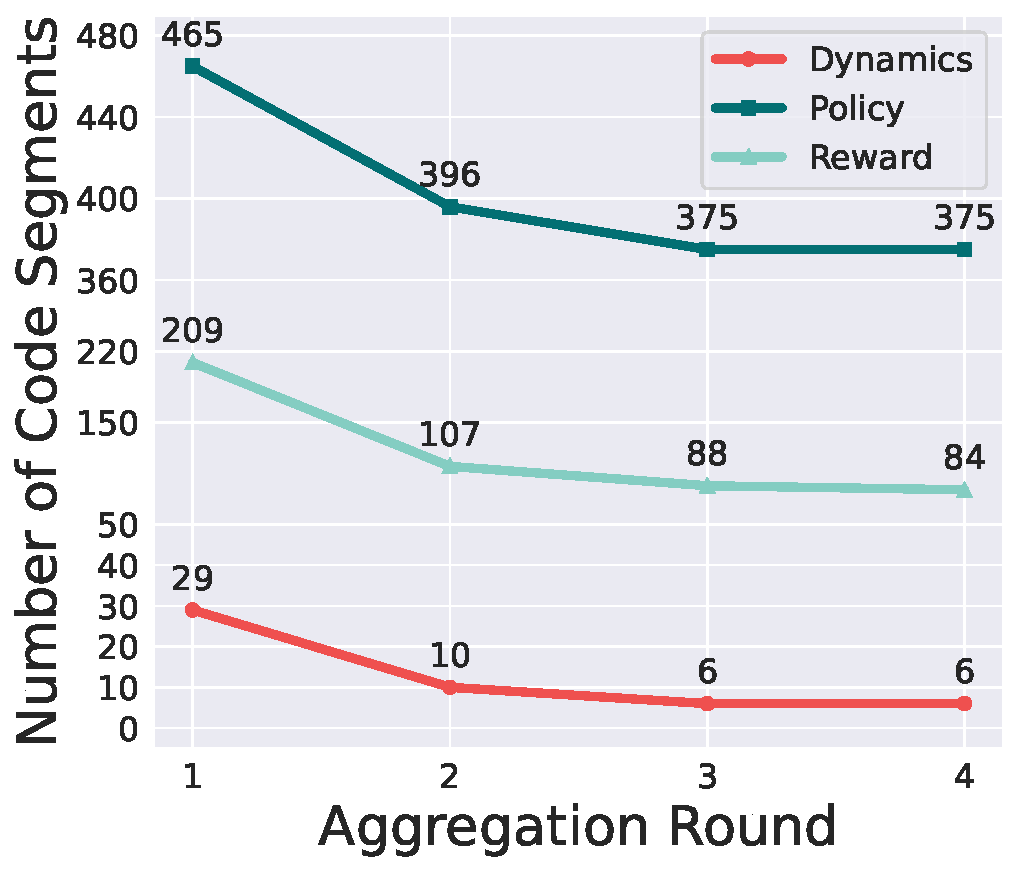
\includegraphics[width=0.85\linewidth]{fig/code_segment_reduction_aggregation.pdf}
        \caption{Knowledge Segment Aggregation.}
        \label{fig:code_segment}
    \end{center}
    \vspace{-3.6cm}
\end{wrapfigure}
According to Section.~\ref{sec:book_content_understanding}, we perform an iterative process of code extraction and aggregation to understand the football textbooks and obtain executable knowledge. Figure.~\ref{fig:code_segment} shows the reduction in the number of code segments for dynamics, policy, and reward functions over the aggregation rounds. Through iterative aggregation, the number of code segments decreases significantly, which helps condense the extracted knowledge into a more compact and coherent form. 

% In addition, we observe that as the number of aggregation rounds increases, the length of the code segment contents also grows, which can be found in the examples and details provided in the Appendix~\ref{app:code_aggregation}.



% What are the results of code extraction: 
% \begin{itemize}
%     \item shows the number of codes of different functions.
%     \item show examples.
% \end{itemize}

% Show the reduction progress of code aggregation.
% \begin{itemize}
%     \item iteration and number of code.
%     \item example of final results.
% \end{itemize}



% \begin{figure}
%     \vspace{-3em}
%     \centering
%     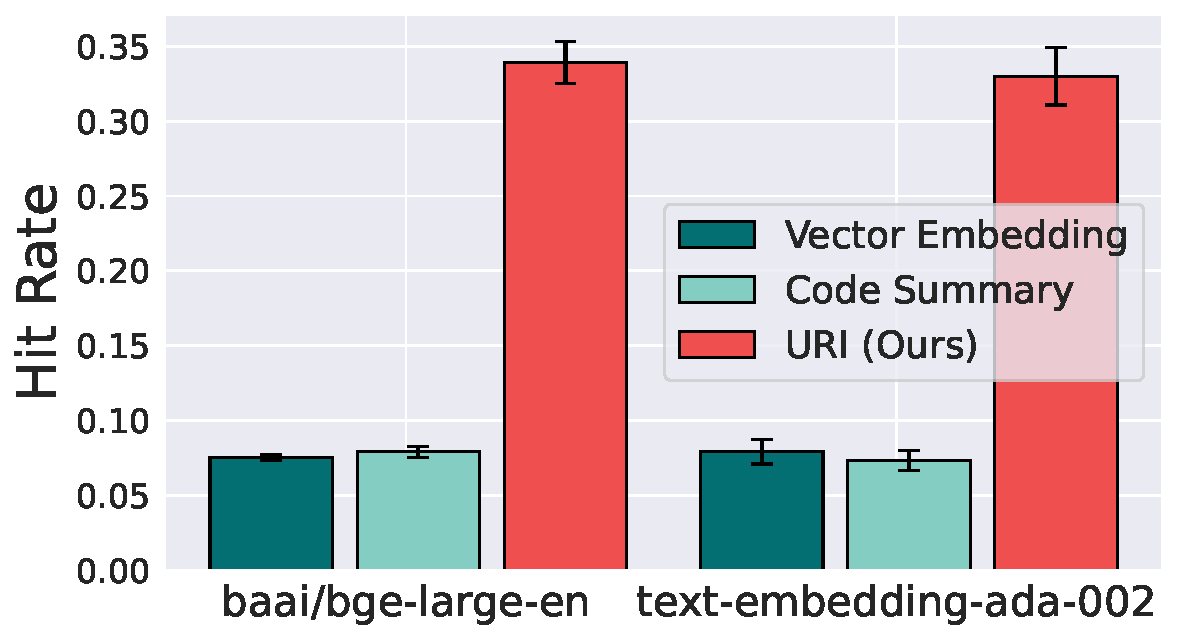
\includegraphics[width=0.4\linewidth]{fig/hitrate.pdf}
%     \hspace{10mm}
%     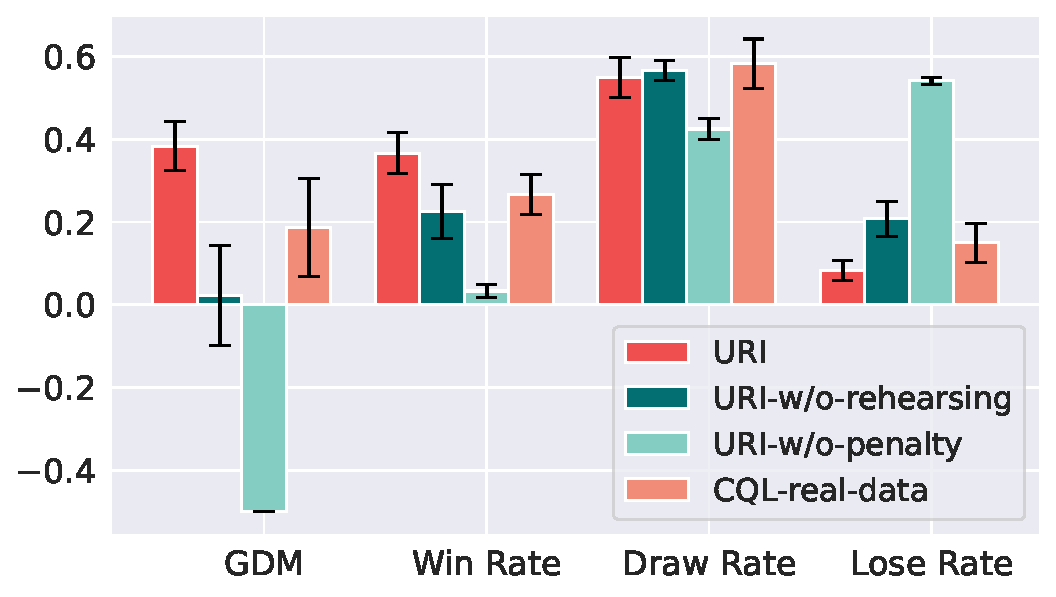
\includegraphics[width=0.4\linewidth]{fig/exp/first_version.pdf}
%     \caption{(a).~Comparison of different code retrieval methods on two pre-trained language models. (b).~Performance comparison of different URI framework variants in the GRF. This figure illustrates the win, draw, and lose rates of the four configurations. The error bars in the figure indicate the standard deviation from the mean performance for each configuration in three random seeds.}
%     \label{fig:hitrate}
%     \vspace{-0.5cm}
% \end{figure}




% \begin{figure}
% \vspace{-3em}
% \centering
% \begin{subfigure}{0.4\linewidth}
% \centering
% 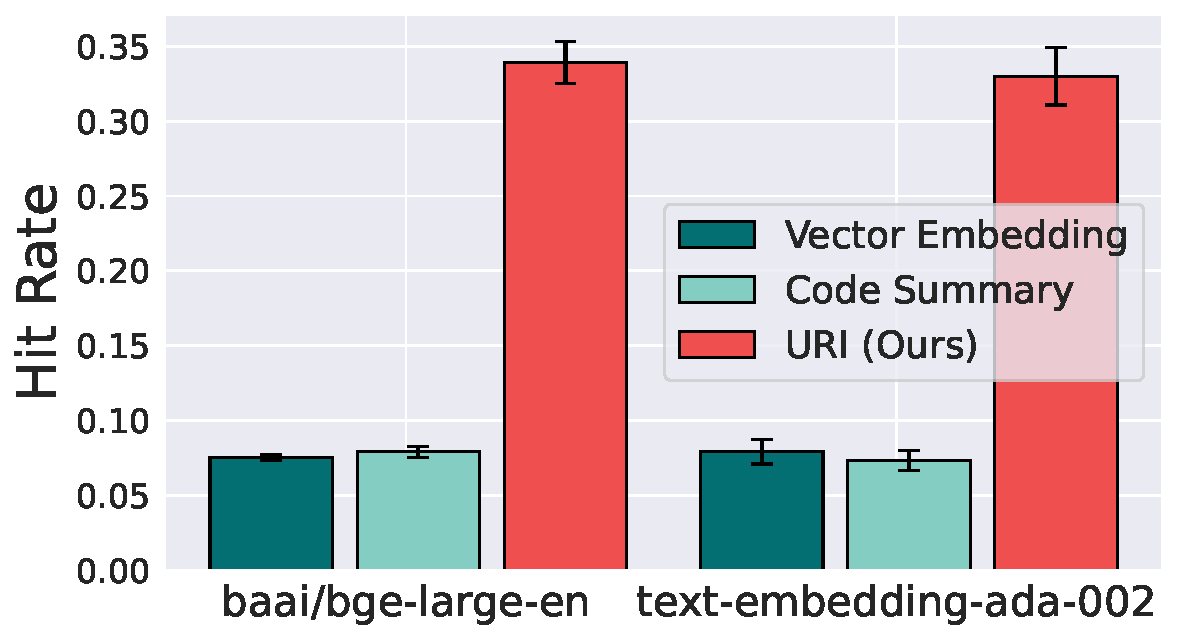
\includegraphics[width=\linewidth]{fig/hitrate.pdf}
% \caption{}
% \label{fig:hitrate_a}
% \end{subfigure}
% \hspace{10mm}
% \begin{subfigure}{0.4\linewidth}
% \centering
% 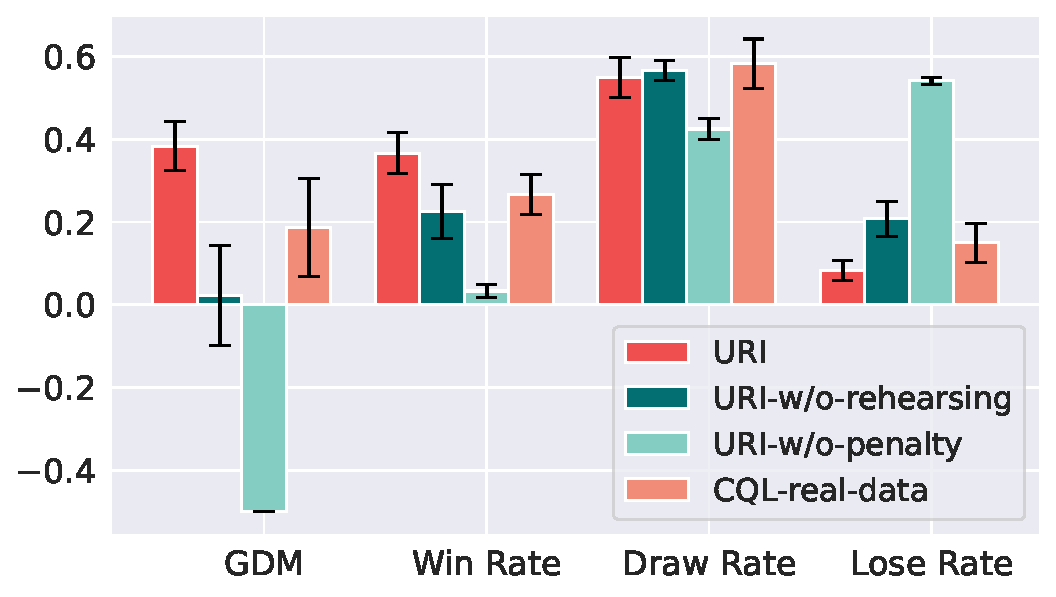
\includegraphics[width=\linewidth]{fig/exp/first_version.pdf}
% \caption{}
% \label{fig:hitrate_b}
% \end{subfigure}

% \caption{(a).~Comparison of different code retrieval methods on two pre-trained language models. (b).~Performance comparison of different URI framework variants in the GRF. This figure illustrates the win, draw, and lose rates of the four configurations. The error bars in the figure indicate the standard deviation from the mean performance for each configuration in three random seeds.}
% \label{fig:hitrate}
% \vspace{-0.5cm}
% \end{figure}



\subsection{Correlation between Knowledge Embedding and Current State Embedding}
\label{exp:emb}

% \begin{wrapfigure}[16]{l}{0.40\textwidth}
% \vspace{-0.3cm}
%     \begin{center}
%         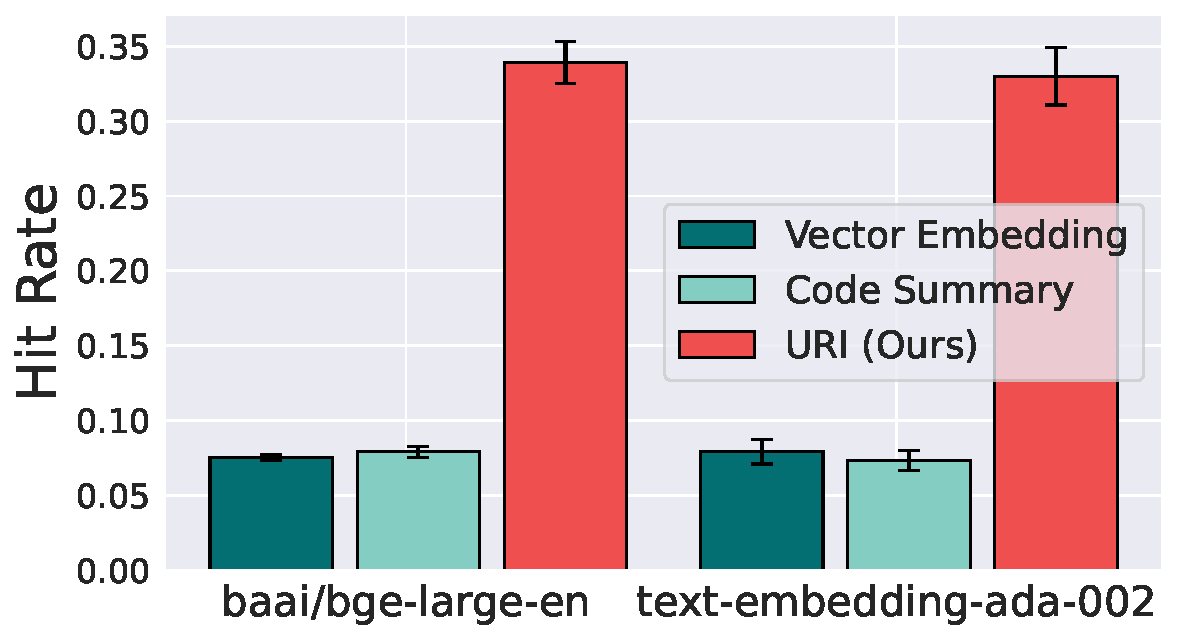
\includegraphics[width=\linewidth]{fig/hitrate.pdf}
%         \caption{Comparison of different code retrieval methods on two pre-trained language models.}
%         \label{fig:hitrate}
%     \end{center}
% \end{wrapfigure}

% In Section.~\ref{sec:sbksr}, we discussed the importance of retrieving relevant code segments based on the current state for effective knowledge instantiation in our PLfB framework. Standard RAG techniques, which directly compare the embeddings of the query (current state) and the documents (code segments), may not work well in this scenario due to the modality gap between the state description and the code content. To address this issue, we proposed the 'obs\_matching' method, which learns a dedicated matcher to score the relevance between the state and the code segments. This matcher is trained to bridge the modality gap and improve the correlation between the state embedding and the code embedding.

To validate the effectiveness of our code embedding method mentioned in Section.~\ref{sec:sbksr}, we conducted experiments comparing it with two baselines: \textbf{Vector Embedding}, which directly compares the state and code embeddings, and \textbf{Code Summary}, which first summarizes the code segments before comparing the embeddings. We evaluate the top-15 hit rate in a hand-crafted test dataset. The observations and actions in the dataset we used are collected by the rule-based policy interacting with the real environment, while the ground-truth codes are labeled by GPT and aggregated using a similar way as in Section.~\ref{sec:book_content_understanding}.
As shown in Figure.~\ref{fig:hitrate}(a), our method significantly outperforms the other two baselines on both pre-trained language models. The hit rate, which measures the proportion of relevant code segments retrieved, is consistently higher for URI across all three random seeds, demonstrating its robustness and superiority in improving the correlation between the state embedding and the code embedding. These results highlight the importance of learning a dedicated matcher for effective code retrieval in our framework. 


% This section examines the interplay between code embedding and current state embedding in our Policy Learning via Reading (PER) framework, with a specific focus on the impact of fine-tuning on code retrieval effectiveness. Understanding this relationship is critical for optimizing the agent's performance in extracting and utilizing knowledge from textual sources for decision-making in a simulated football environment.

% \begin{figure}[ht]
% \centering
% \includegraphics[width=0.75\linewidth]{code_state_embedding_correlation.png}
% \caption{Illustration of the correlation between code embedding and current state embedding before and after fine-tuning in the PER methodology.}
% \label{fig:code_state_embedding}
% \end{figure}

% To demonstrate the capacity of our system to retrieve effective information from code, we compare the results before and after fine-tuning. Metrics such as accuracy or correctness in code retrieval can be used to quantify this impact. Figure.~\ref{fig:code_state_embedding} showcases that fine-tuning significantly enhances the alignment between code embedding and the current state embedding, indicating more accurate and relevant information retrieval post-fine-tuning.

% \begin{figure}[ht]
% \centering
% 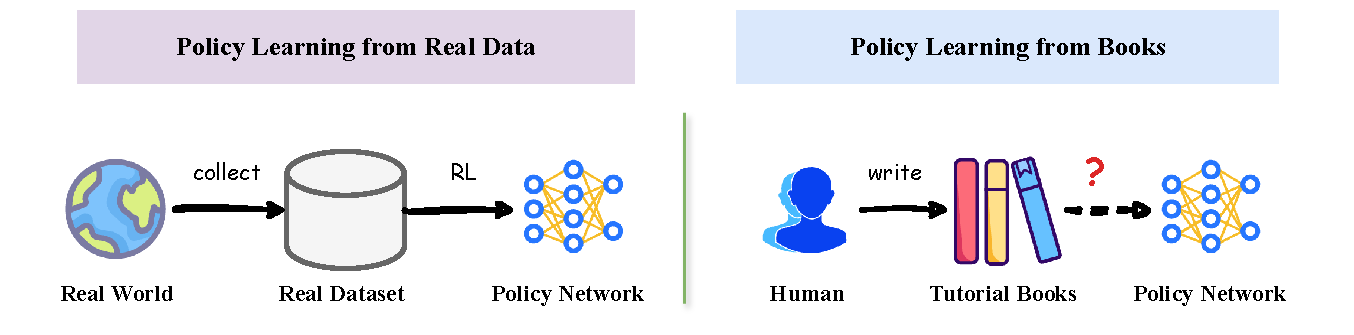
\includegraphics[width=0.75\linewidth]{fig/PER-problem.pdf}
% \caption{Example.}
% \label{fig:code_state_embedding}
% \end{figure}

 % Examining specific instances of code retrieval before and after the fine-tuning process provides practical insights. Initially, the retrieved codes may only partially align with the current state requirements, reflecting a generalized understanding. Post-fine-tuning, the codes demonstrate a high degree of specificity and relevance, indicating a more nuanced understanding and application of football strategies and tactics as per the current game state.
 
% \textbf{[level 2] Comparing Different Fine-Tuning Techniques:} Different fine-tuning techniques can yield varied results in terms of code retrieval efficiency and accuracy. By comparing techniques such as supervised fine-tuning, unsupervised fine-tuning, and reinforcement learning-based fine-tuning, we can determine the most effective method for aligning code and state embeddings in our PER framework. This analysis not only enhances the performance of the agent but also contributes to the broader understanding of fine-tuning impacts in language model-based learning systems.
% \begin{wrapfigure}[18]{r}{0.5\textwidth}
% \vspace{-1cm}
%     \begin{center}
%         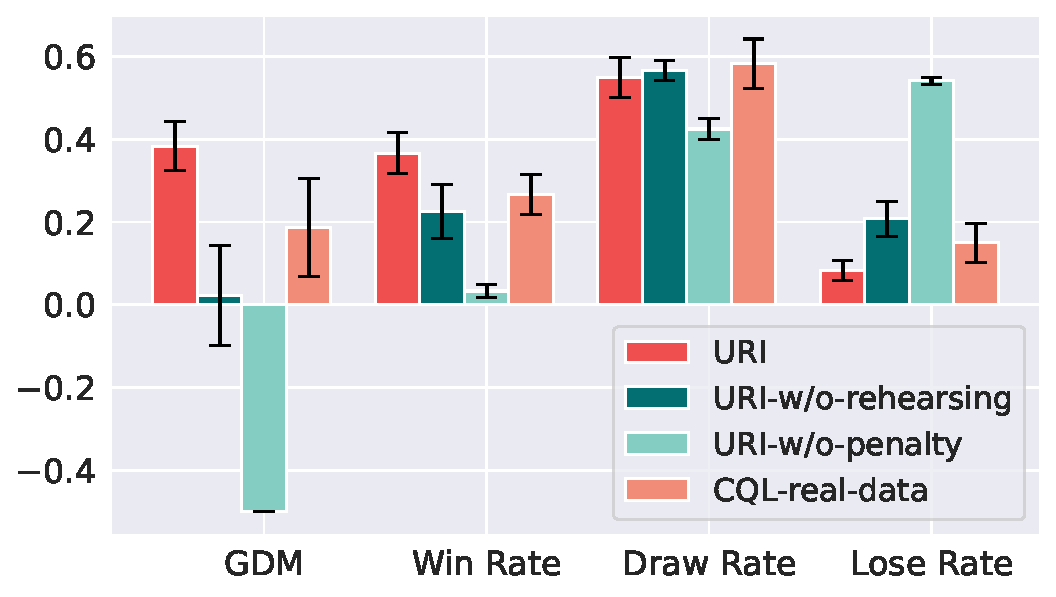
\includegraphics[width=\linewidth]{fig/exp/first_version.pdf}
%         \caption{Performance comparison of different URI framework variants in the GRF. This figure illustrates the win, draw, and lose rates of four configurations. The error bars in the figure indicate the standard deviation from the mean performance for each configuration in three random seeds.}
%         \label{fig:ablation}
%     \end{center}
% \vspace{-0.6cm}
% \end{wrapfigure}


\begin{figure}[t]

\centering
\vspace{-7mm}
\begin{tabular}{cc}
    \subfigure[]{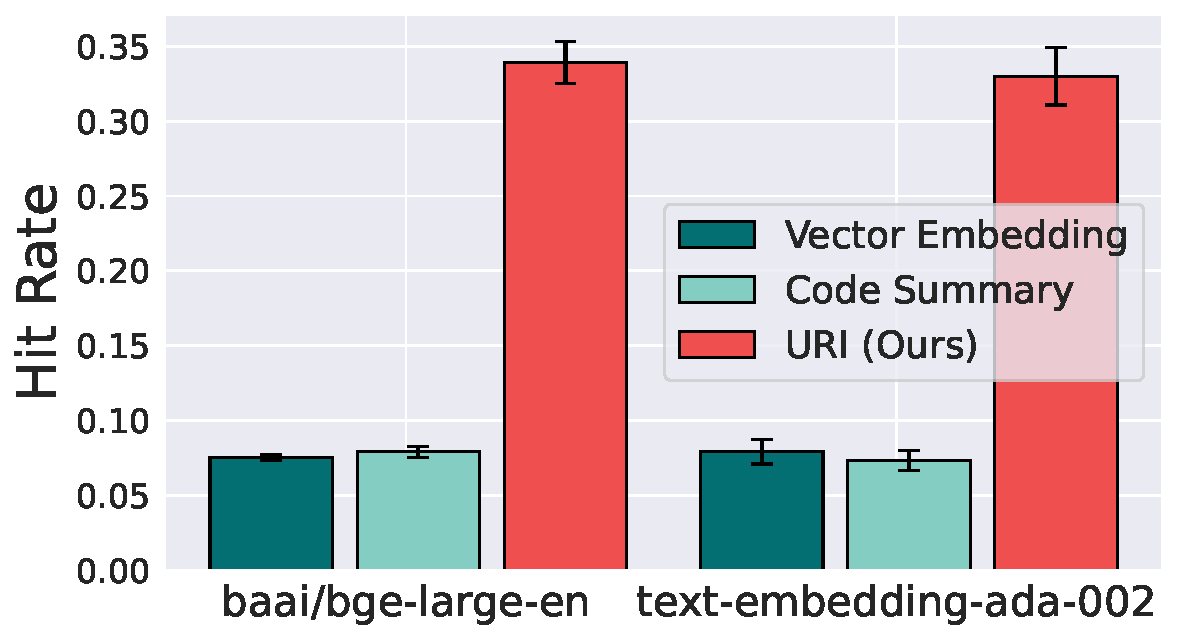
\includegraphics[width=0.45\linewidth]{fig/hitrate.pdf}} 
    \hspace{5mm}
    \subfigure[]{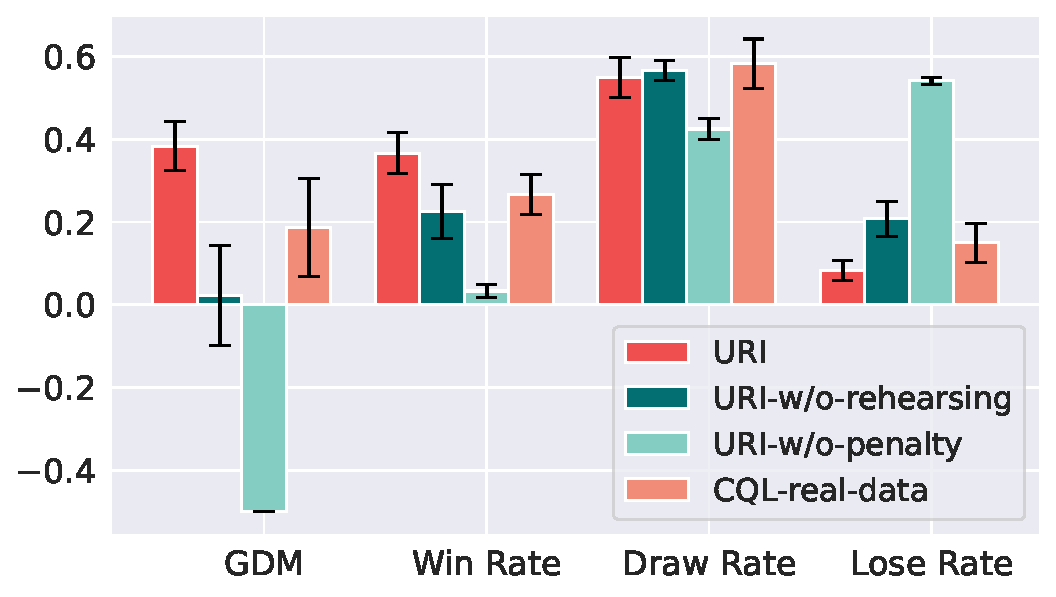
\includegraphics[width=0.45\linewidth]{fig/exp/first_version.pdf}} 
\end{tabular}
\caption{(a).~Comparison of different code retrieval methods on two pre-trained language models. (b).~Performance comparison of different variants of the URI framework in the GRF. This figure illustrates the average GDM, win, draw, and lose rates among the three levels of built-in AIs. The error bars in the figure indicate the standard deviation from the mean performance for each configuration in three random seeds.}
\label{fig:hitrate}
\vspace{-0.5cm}
\end{figure}



\subsection{Tracing the Data Generation Process}

\begin{figure}[h]
    % \centering
    \hspace{-9mm}
    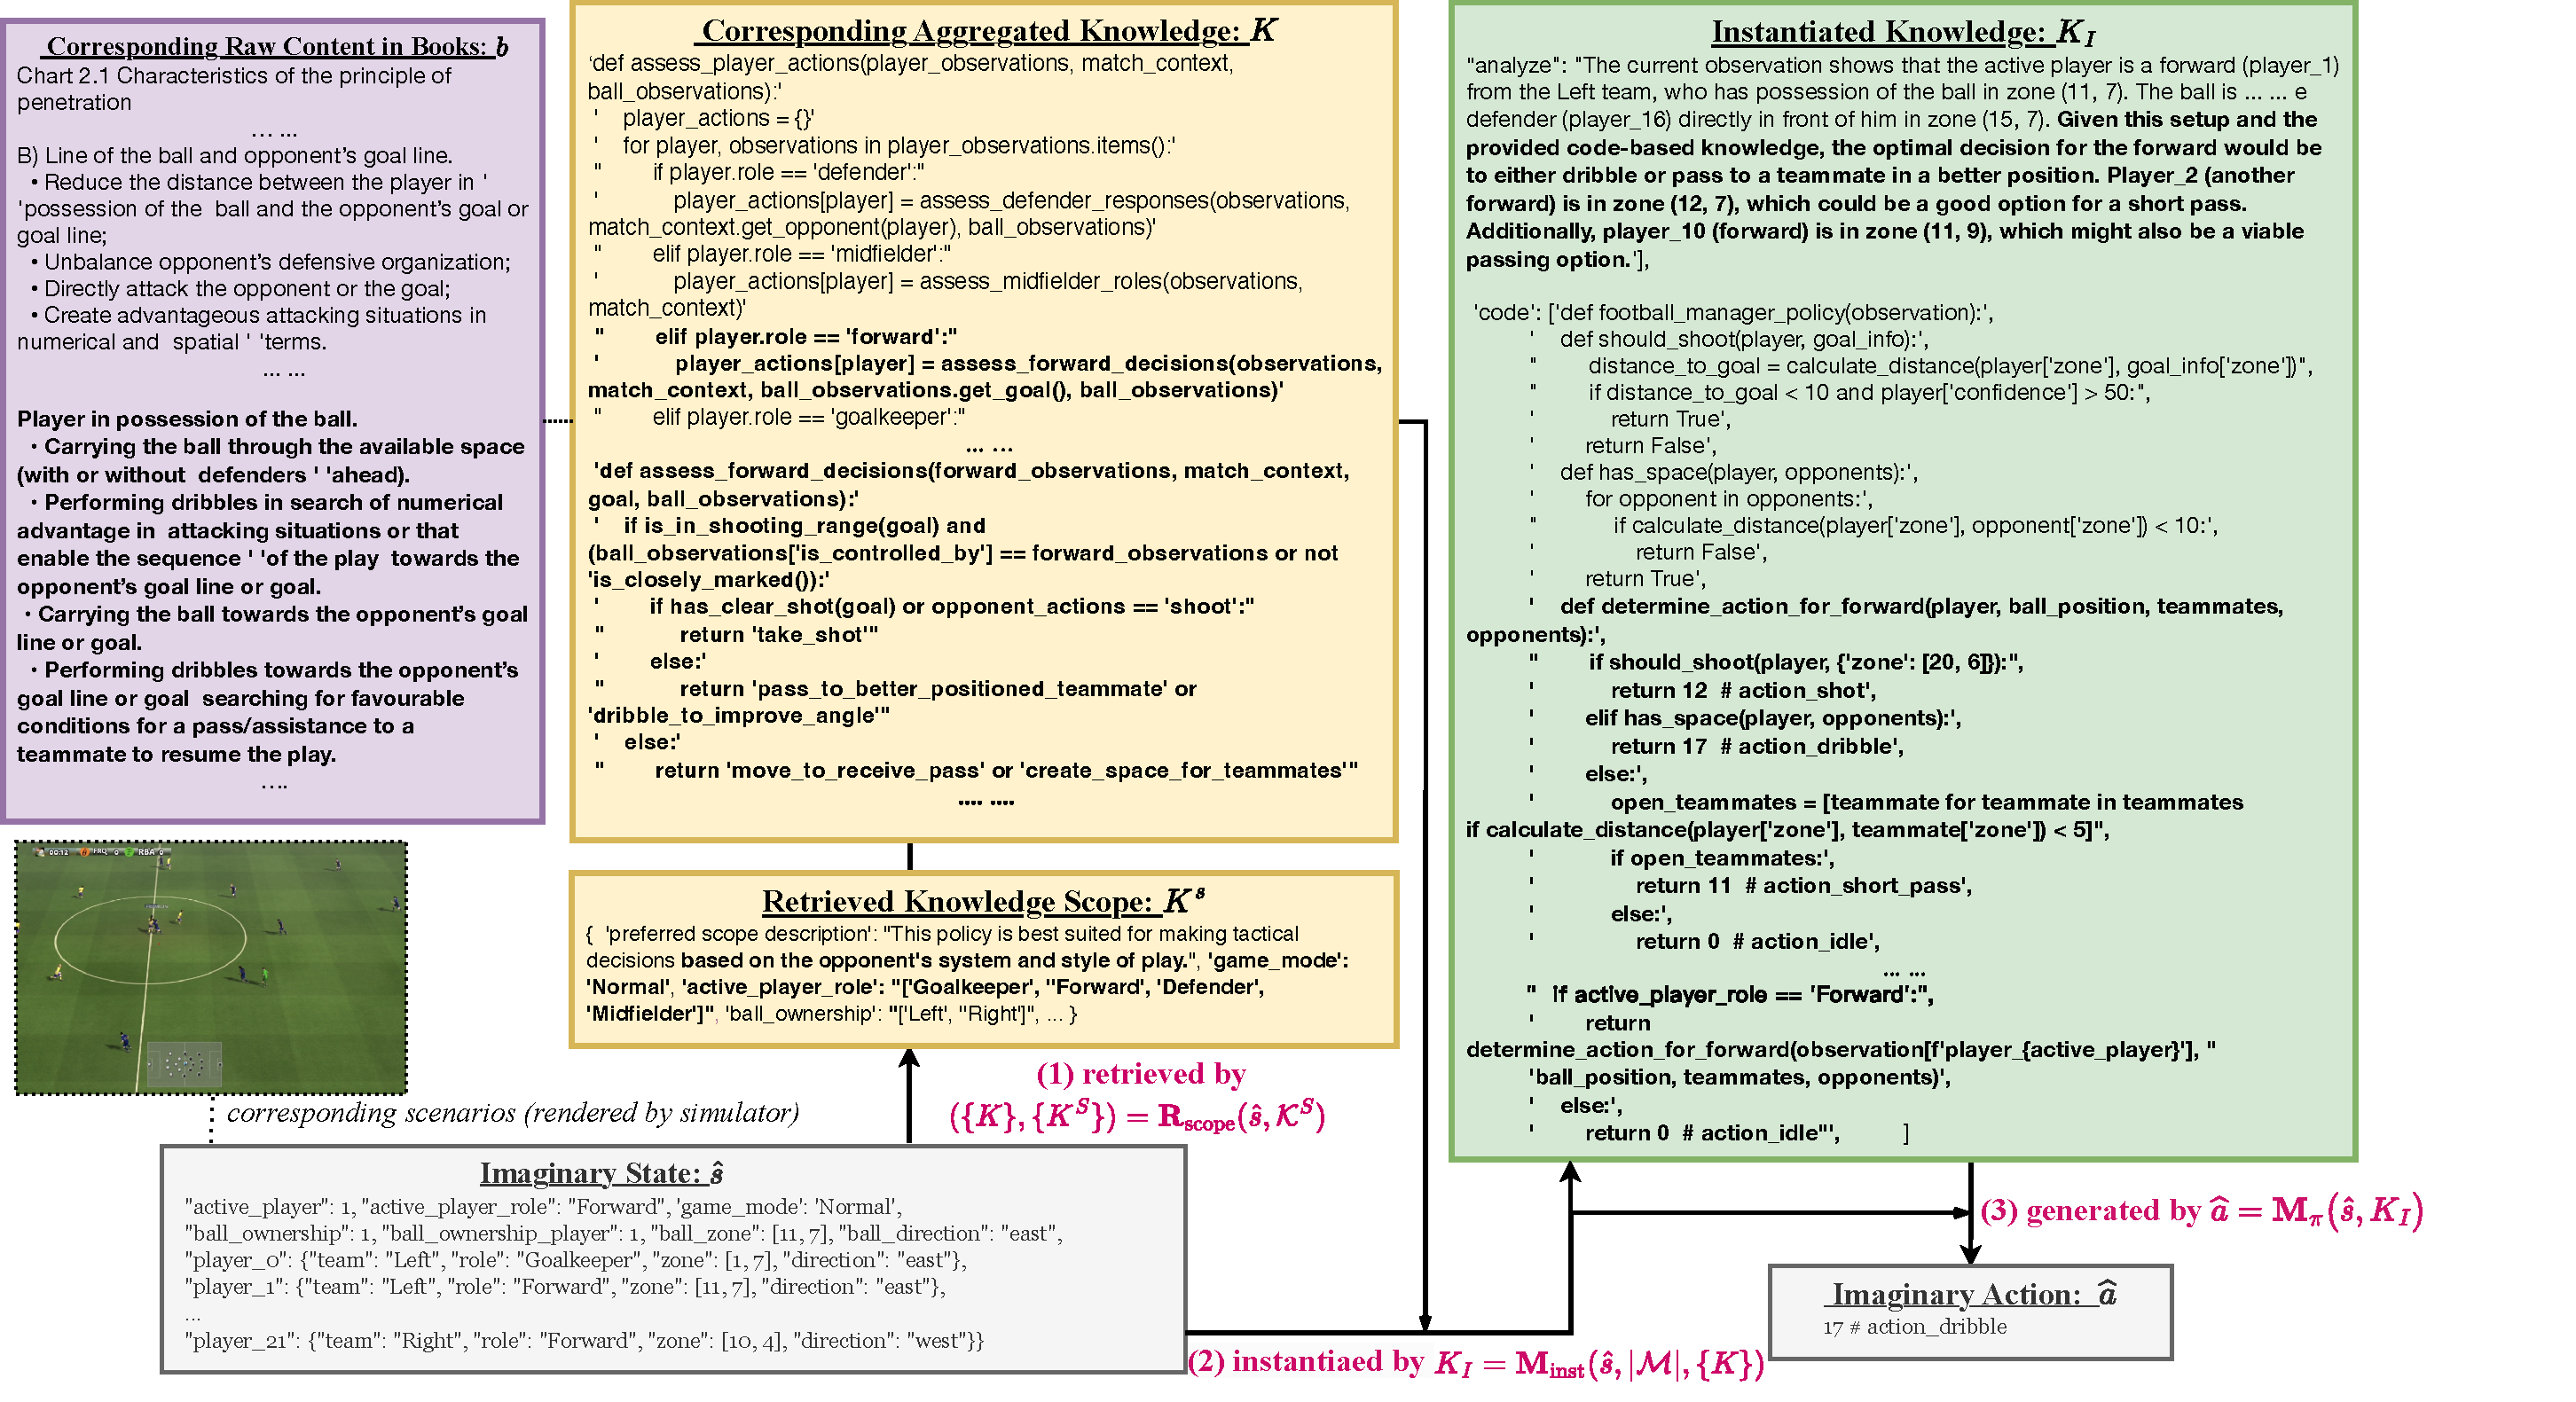
\includegraphics[width=1.2\textwidth]{fig/example2.pdf}
    \caption{Results of the imaginary action generation process. The imaginary state $\hat s$ is collected from the real environment, which is the 12 timestep of a football game, while the rendered image is the corresponding scenario generated by the simulator. The imaginary action is ``dribble'', where the logic is supported by the ``has\_space'' branch in $K_I$. Based on this, we \textbf{bold} the relevant information in the predecessor nodes and skip irrelevant information with the ellipsis ``... ...''.}
    \label{fig:data_gen_demo}
    \vspace{-1mm}
\end{figure}
In \algo, it is crucial to guarantee that the imaginary data include states, actions, and rewards. The task is non-trivial since it has to involve several transformations to align the gap between textual contents in books and decision-making trajectories in MDP. To verify the effectiveness of the data generation process, we trace how $\llm_\pi$ outputs an imaginary action $\hat a$ on an imaginary state $\hat s$, which is actually collected at the start of a football game in GRF. We record all the intermediate outputs to trace the action generation process. The result is shown in Figure.~\ref{fig:data_gen_demo}.   It is clearly shown that the output action ``dribble'' is fully supported by the logic in``has\_space'' branch in $K_I$, ``assess\_forward\_decisions'' function in $K$, and the paragraph of ``Player in possession of the ball'' in the raw content of tutorial books. However, we would like to point out that there are also some examples that demonstrate LLMs having hallucinations in generation, and the retrieved module might also miss the ground-truth piece of knowledge. More results are provided in Appendix~\ref{app:example}. These results indicate the necessity of introspecting in \algo. The relevant ablation studies are in Section.~\ref{exp:abl}.
% 有效的
% 局限性
% 更多的结果


\vspace{-1mm}
\subsection{Importance of the components in URI}
\label{exp:abl}
% \vspace{-2mm}
% \begin{figure}[h]
% \centering
% 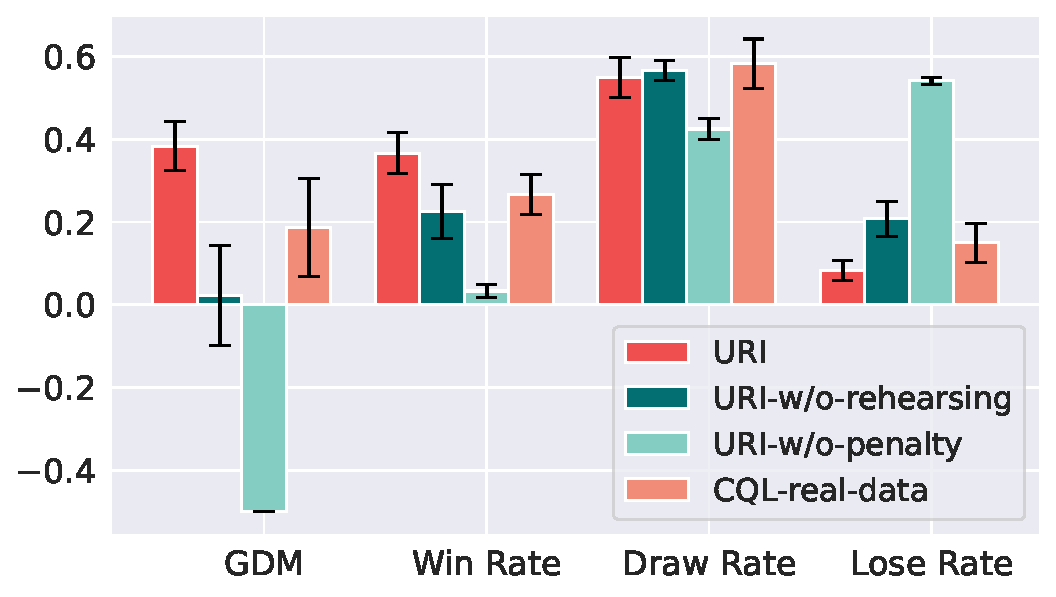
\includegraphics[width=0.7\linewidth]{fig/exp/first_version.pdf}
% \caption{}
% \label{fig:ablation}
% \end{figure}

In this section, we validate the effectiveness of the rehearsing technique presented in Section~\ref{sec:rehearsing} and the CIQL method introduced in Section~\ref{sec:introspecting} through ablation studies. Specifically, we constructed the following variants of the URI framework: (1) \textbf{URI-w/o-rehearsing}, which solves the policy without using the rehearsing dataset and relies on a pre-collected dataset of 7,500 samples for offline RL policy training; (2) \textbf{URI-w/o-penalty}, where penalties  $\eta_\transf$ and $\eta_\rewf$ are zero, same as the standard CQL for policy learning; (3) \textbf{CQL-real-data}, where we collect real data of equivalent scale to the rehearsing-generated data using rule-based AI and apply standard CQL for offline RL policy training. The results are shown in Figure.~\ref{fig:hitrate}(b).

Firstly, URI-w/o-rehearsing demonstrates that without generating a substantial amount of imaginary data through rehearsing, solely relying on offline RL algorithms to train a policy with our pre-collected 7,500 samples is ineffective. The results indicate that it cannot even beat the AI on Easy difficulty, though it still performs better than a random strategy. URI-w/o-penalty underscores the importance of penalizing the uncertain aspects of the outcomes generated from the imaginary data. Neglecting this penalty leads to results worse than those of URI-w/o-rehearsing. 
Finally, our method slightly outperforms CQL-real-data. We attribute this improvement to the strategies inferred from prior knowledge by LLMs, which are partially superior to built-in AI behaviors, or possibly because LLMs generate more diverse data. This illustrates the considerable potential of \topic.


% ablation studies among different components in offline RL.
% \begin{itemize}
%     \item without uncertainty estimator
%     \item without imaginary data.
%     \item different hp-parameters selection [lp].
% \end{itemize}

% \subsection{Ablation studies [ziyan-baseline]}

% [figure]

% \begin{itemize}
%     \item PER
%     \item without-RL: book-rag-$\pi$ [done]
%     \item  without-book-information: GPT-imgdata-$\pi$ [lp]
% \end{itemize}
\vspace{-1mm}
\subsection{Efficiency in inference}
% \vspace{-2mm}
% Table \ref{tab:inference_time} compares the inference time per action for different methods. Our URI approach takes only 0.50 seconds on average to choose an action, which is significantly faster than using LLMs directly as agents (2.84 seconds) or with retrieval-augmented generation (RAG) (4.12 seconds). This makes URI more suitable for real-time decision making in the football simulator. The efficiency gain comes from the fact that URI distills the knowledge from the LLM into a compact policy network, which can be executed quickly without the need for expensive LLM inference at each step.



\begin{wrapfigure}[7]{r}{0.41\textwidth}
\centering
\vspace{-1cm}
\begin{minipage}{0.41\textwidth}
\begin{table}[H]
\caption{Comparison of inference time per action for different methods.}
\centering
\begin{tabular}{ll}
\hline
           & Time Cost(s)
                  \\ \hline


LLM-as-Agent  & 2.84 $\pm$ 0.71  \\

LLM-RAG & 4.12 $\pm$1.46 \\

URI & \textbf{0.009 $\pm$ 0.0004} \\
\hline
\end{tabular}
\vspace{-2cm}
\label{tab:inference_time}
\end{table}
\end{minipage}
\end{wrapfigure}

In real-time decision-making tasks such as playing football, the efficiency of the policy is crucial. We compare the inference time per action for different methods in Table \ref{tab:inference_time}. Our approach takes only 0.009 seconds on average to choose an action, which is significantly faster \textbf{at least 300 times} than using LLMs directly as agents (2.84 seconds) or with retrieval-augmented generation (RAG) (4.12 seconds). This makes URI more suitable for real-time decision-making in the football simulator. The efficiency gain comes from the fact that URI distills the knowledge from the LLM into a compact policy network, which can be executed quickly without the need for expensive LLM inference at each step.


% \subsection{Amount of Imaginary Dataset Used}

% % [figure]

% Show the relationship between the amount of offline dataset used, the imaginary dataset used, and the performance of the learned policy.


\vspace{-1mm}
\subsection{Imaginary Dataset Visualization}  
\begin{wrapfigure}[14]{r}{0.35\textwidth}
\vspace{-0.7cm}
    \begin{center}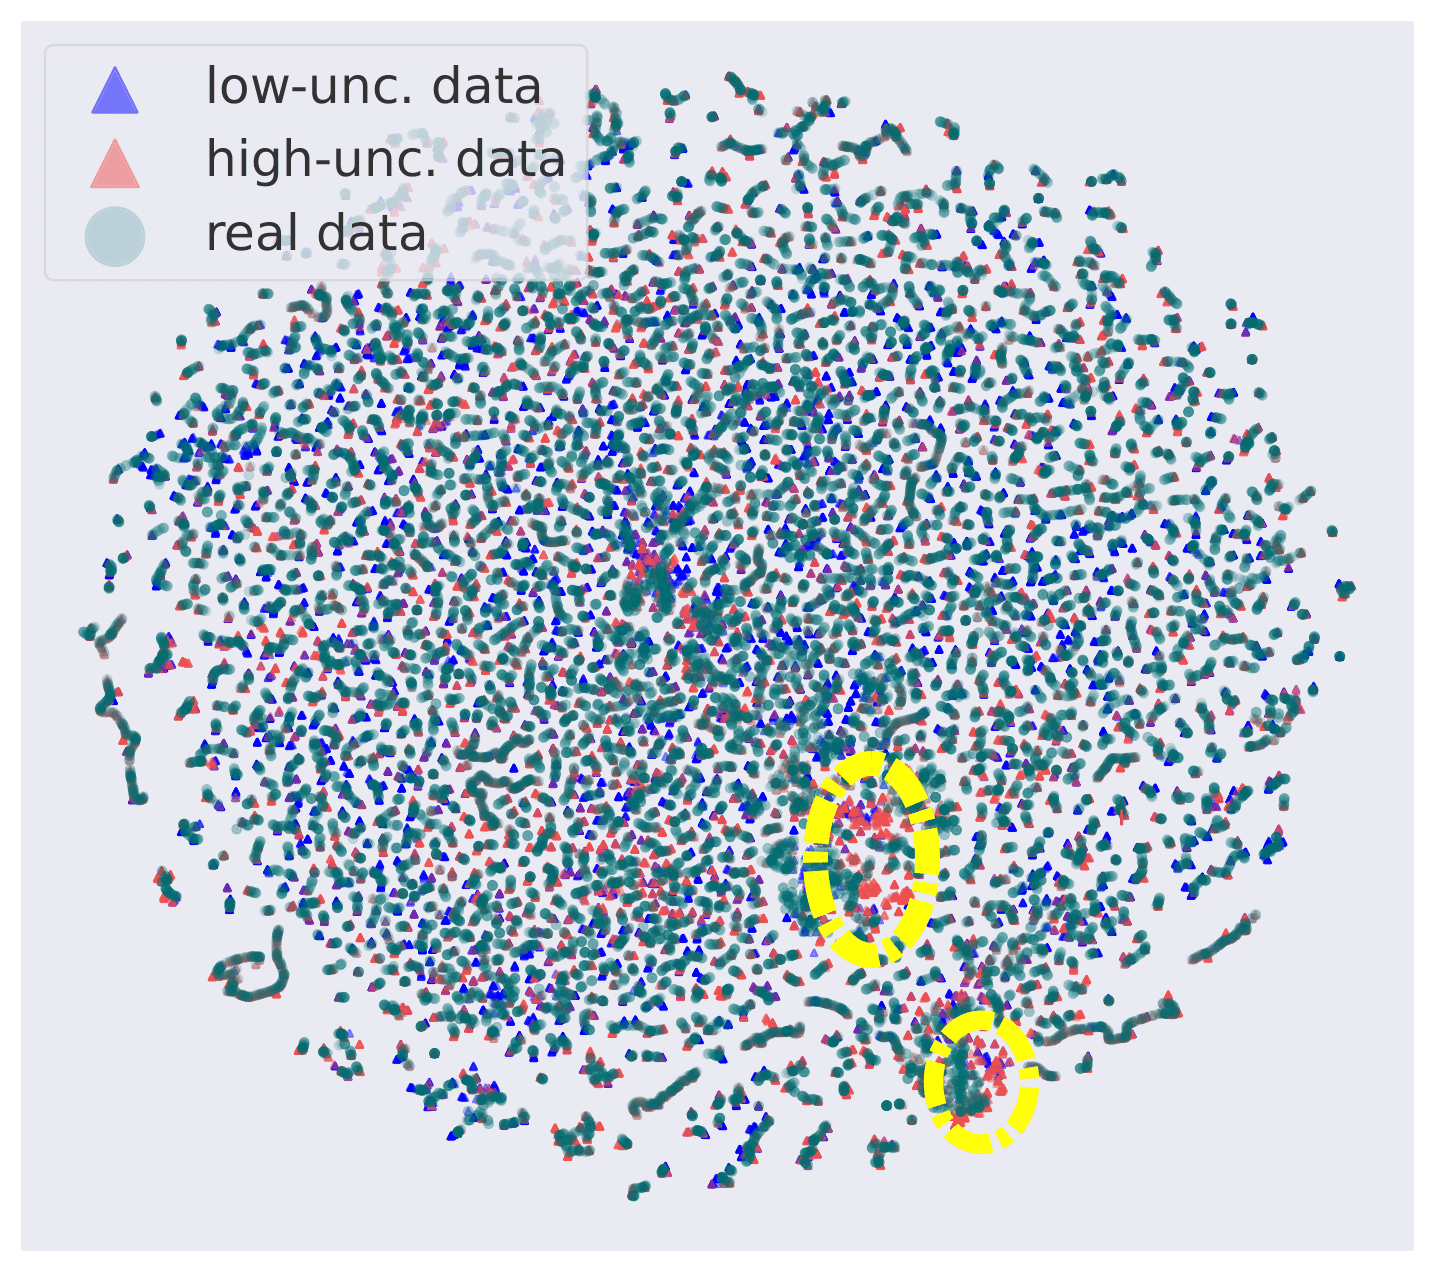
\includegraphics[width=0.95\linewidth]{fig/exp/tsne-1.png}
        \caption{Visualization of the projected distributions for real and imaginary datasets. }
        \label{fig:vis}
    \end{center}
    \vspace{-0.2cm}
\end{wrapfigure}
In this section, we visualize the imaginary dataset to analyze the quality of its generation and uncertainty estimation.  We choose t-SNE~\citep{mataten2008tsne} as the visualization method and project the imaginary dataset and a real dataset collected by the rule-based policy into 2-d space for comparison. The results are in Figure.~\ref{fig:vis}. The "real data" marks the data collected by the rule-based policy, while "low-unc. data" and "high-unc. data" represent segments of the imaginary dataset categorized by their uncertainty scores $R_\transf$ and $R_{\rewf}$ falling within the lower and upper 50\% percentiles, respectively. The real data and the imaginary data follow a similar data distribution, which indicates the effectiveness of the rehearsing process in \algo. Besides, as highlighted by the yellow dashed circles, the uncertainty score also identifies parts of the clusters that are out of the real data distribution, which will be penalized when introspecting via CIQL. The results give us more confidence about the effectiveness of the URI framework.

% Besides, we use t-SNE~\citep{mataten2008tsne} to project imaginary dataset and a real dataset collected by the rule-based policy for comparison, where the results are in Figure.~\ref{fig:vis}. The "real data" is collected by the rule-based policy, while "low-unc. data" and "high-unc. data" represent segments of the imaginary dataset categorized by their uncertainty scores $R_\transf$ and $R_{\rewf}$ falling within the lower and upper 50\% percentiles, respectively. It is easy to see that the real data and the imaginary dataset are overall in the same data distribution, which indicates the effectiveness of the rehearsing process in \algo. Besides, as highlighted by the yellow dashed circles, the uncertainty score also identifies parts of the clusters that are out of the real data distribution, which will be penalties when introspecting via CIQL. The results give us more confidence about the effectiveness of the URI framework.



% \begin{itemize}
%     % \item description of the implementation, how to select the start point, how to start and end.
%     \item vis the distribution of generated dataset and real dataset via some projection;
%     % \item Show one example of retrieval, Stage 1, Stage 2: given state, the find codes, stage-1 results, stage-2 results.
% \end{itemize}


\vspace{-1mm}
\section{Conclusion}
\vspace{-1mm}

Inspired by the learning behavior of humans when they try to acquire a new skill, we propose {\topic} that trains an agent from books, instead of numerous interaction data with the real environment. We also implement a practical algorithm of understanding, rehearsing, and introspecting modules to realize such a learning paradigm. The result of deploying our method in a football game environment demonstrates a huge improvement in the winning rate over the baseline methods. This success proves the feasibility of utilizing knowledge stored in various written texts for decision-making agents, which was neglected by the community for a long time. 

We hope that this promising result will initiate more research on {\topic} and we leave more discussion of the limitation and several interesting open problems of this study in Appendix~\ref{app:limi}.

 % further generalize the learning paradigm to materials of other modalities and deploy it in more scenarios.

% \section{Discussion and Open Problems}

% We hope this promising result will initiate more research on {\topic}, including better knowledge extraction and representation, combining it with traditional trial-and-error methods, or introducing other planning modules into the framework. In the following, we would also like to list several open problems for consideration:

% In light of our proposed framework, \algo, for extracting knowledge from textual sources, it is pertinent to consider whether it represents the most effective pipeline currently available. For example, the manner in which knowledge is represented is of paramount importance, prompting us to question whether coding is indeed the most efficient medium for this purpose.

% Acknowledging the synergistic relationship between reading and practical experience in human learning, we are prompted to explore how machines might integrate interaction data into their learning processes. This hybridization of learning strategies may significantly enhance the agent’s decision-making capabilities.

% Furthermore, given the prevalence of multi-modal tutorials in the real world, incorporating multimedia materials such as images and videos into the framework will be a promising next-step study. This expansion will enable a more comprehensive understanding of the subject matter and enrich the learning experience for the agent.

% We are also compelled to investigate other potential applications of the framework beyond the scope of the current experiment. Domains such as cooking and chess, which require both theoretical knowledge and practical skill, could benefit significantly from the integration of the learning paradigm. This exploration opens up exciting avenues for future research and application of the method.







\bibliography{example_paper}
\bibliographystyle{unsrtnat}

%%%%%%%%%%%%%%%%%%%%%%%%%%%%%%%%%%%%%%%%%%%%%%%%%%%%%%%%%%%%

\appendix

\newpage
\appendix


\renewcommand{\thepart}{}
\renewcommand{\partname}{}

\part{\huge{\textbf{Appendix}}} % Start the appendix part
\parttoc % Insert the appendix TOC
\clearpage


\section{Google Research Football (GRF) Tasks Setup}
\label{app:grf}

\begin{figure}[h]
    \centering
    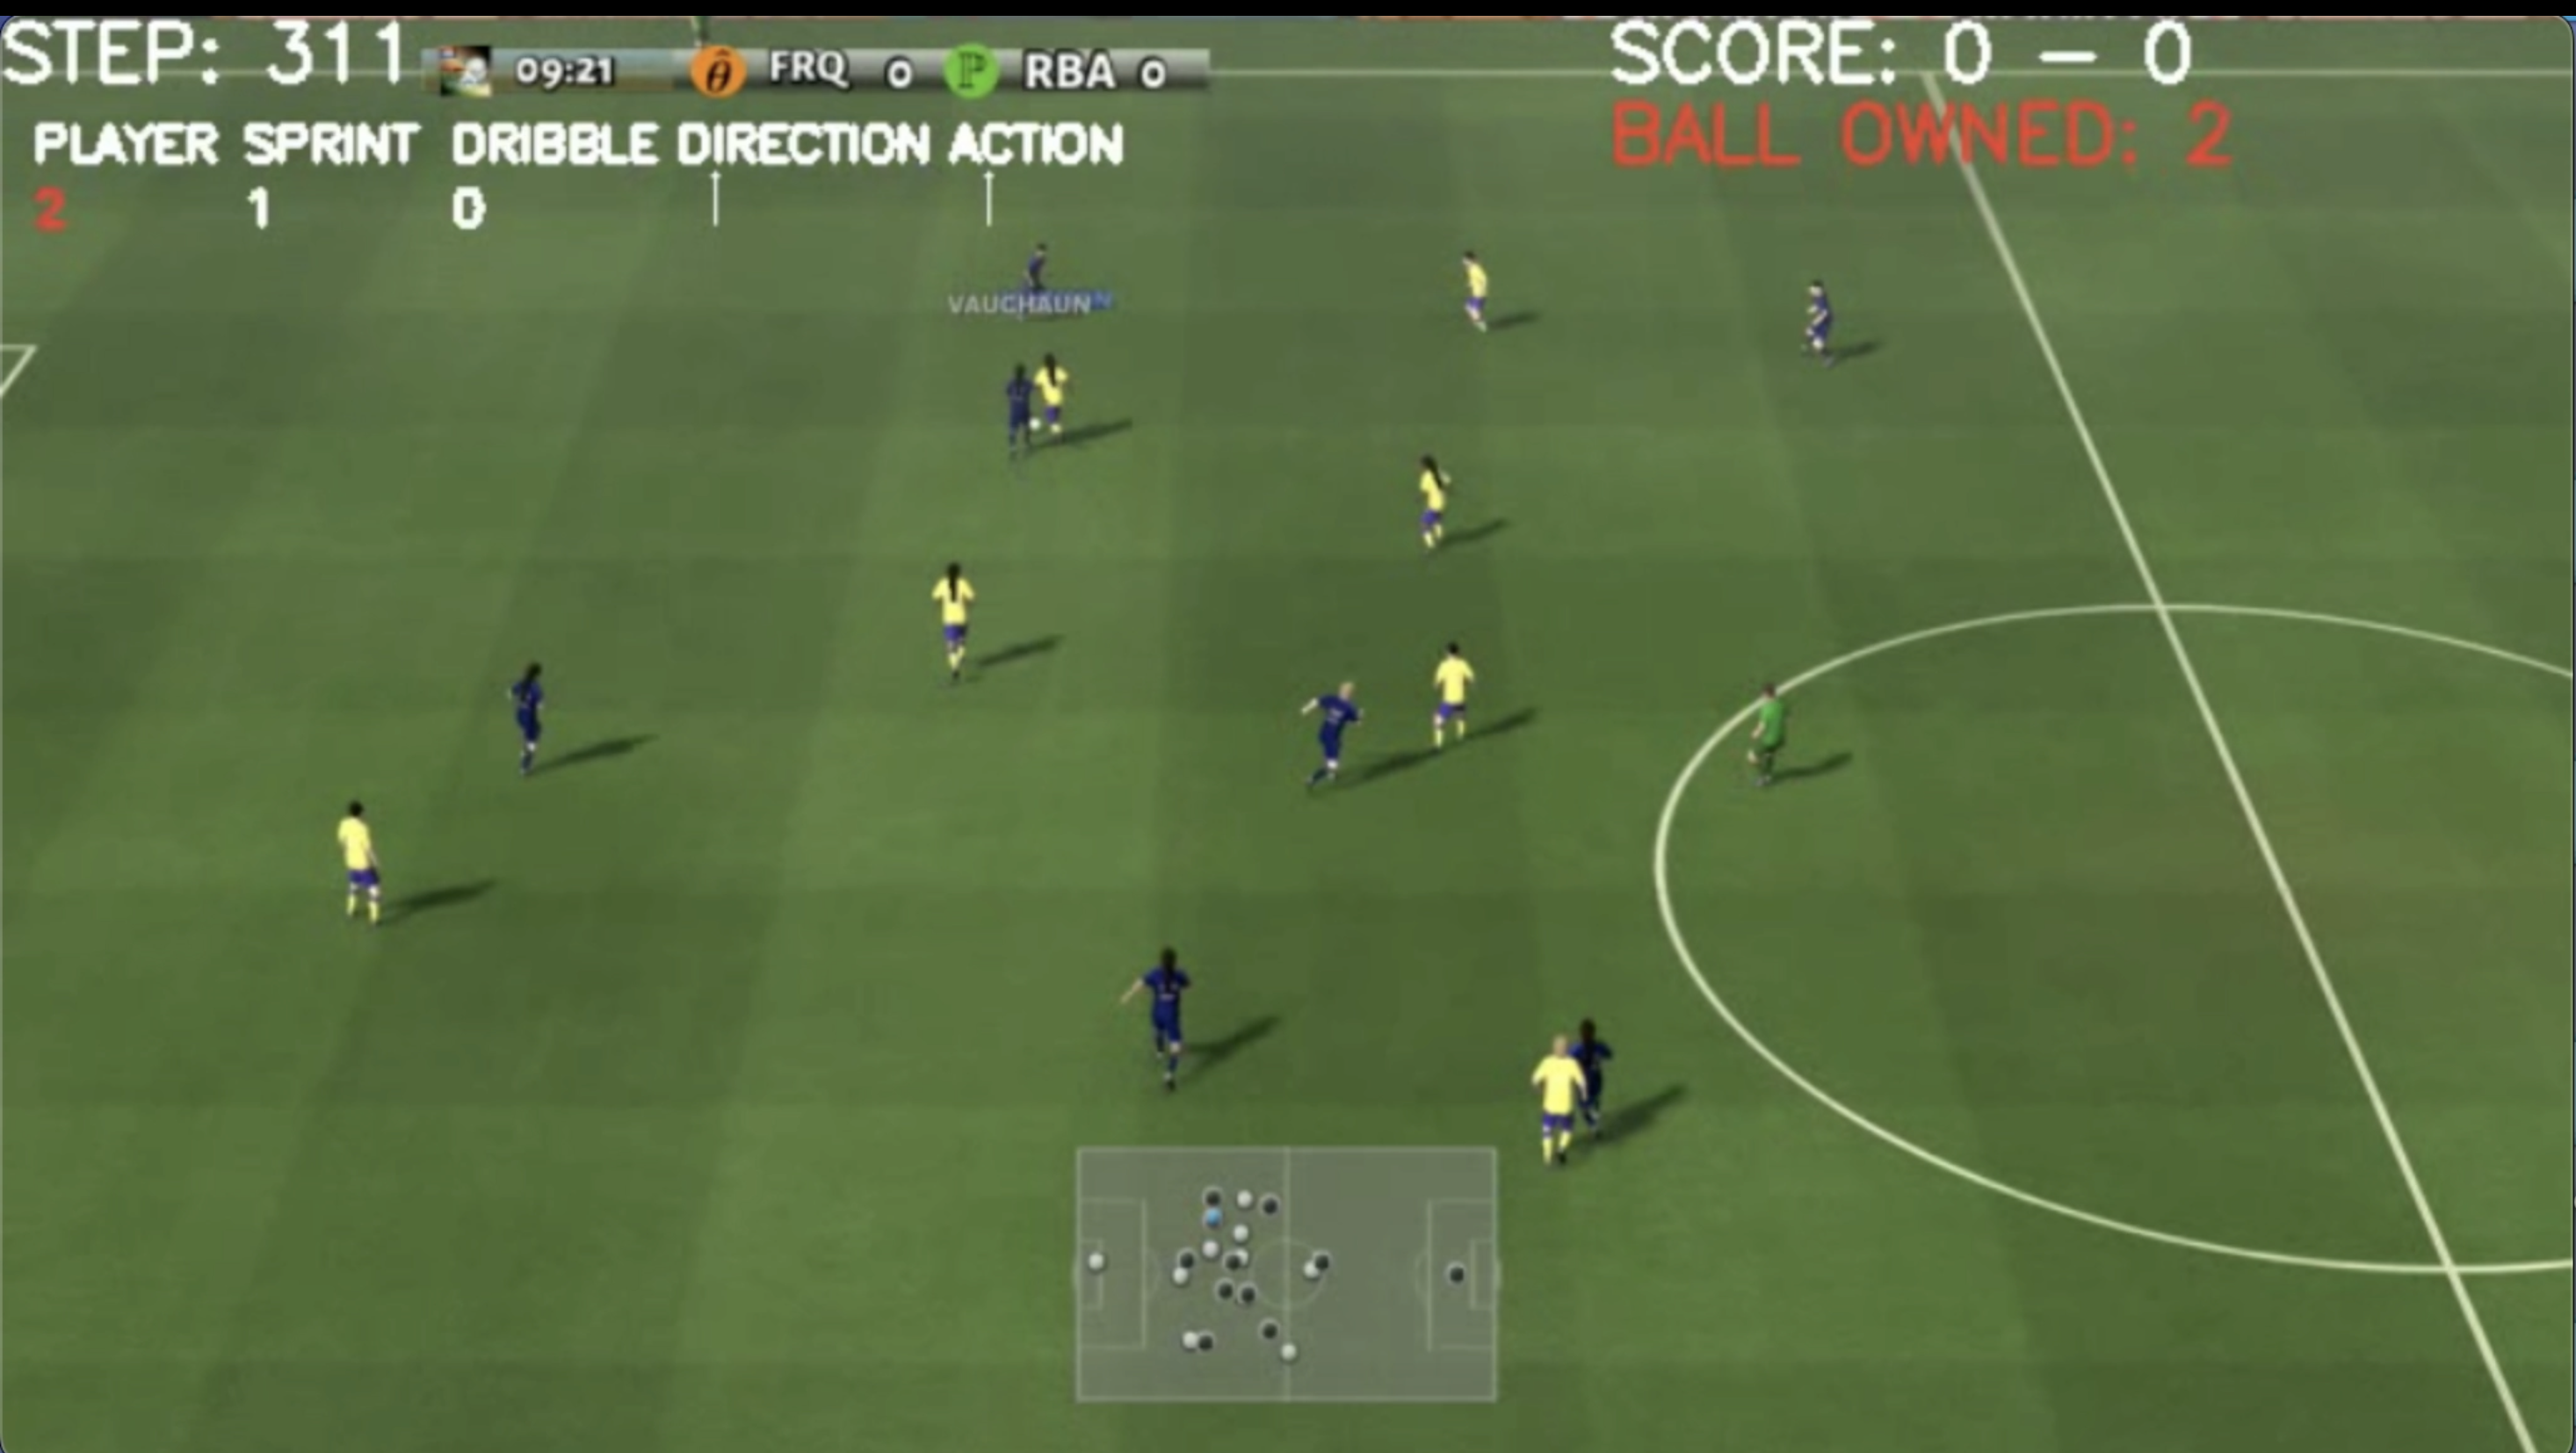
\includegraphics[width=0.75\textwidth]{fig/football_main.png}
    \caption{Illustration of the game in football simulator.}
    \label{fig:football_main}
\end{figure}


In this section, we mainly focus on the GRF implementation\footnote{https://github.com/google-research/football/blob/master/gfootball/} and the modifications we made under this environment. 
\subsection{State Space}


The raw state of each player contains information about the game state, the ball and all players on the pitch. The game state includes scores, game modes indicating free kicks, corner kicks or other game stages, and game time represented as steps. The ball information includes its spatial position, direction, and an indicator for ball ownership (identifying the player and team that possess it). The player information comprises position, direction, roles, yellow card records, and more. For players on the opposite team, positions and directions are mirrored. The details of the raw state are as follows:

\begin{itemize}[leftmargin=*]
\item \textbf{Ball Information:}
\begin{itemize}
\item \texttt{ball} -- $[x, y, z]$ position of the ball.
\item \texttt{ball\_direction} -- $[x, y, z]$ ball movement vector.
\item \texttt{ball\_rotation} -- $[x, y, z]$ rotation angles in radians.
\item \texttt{ball\_owned\_team} -- \{-1, 0, 1\}, where -1 indicates the ball is not owned, 0 denotes the left team, and 1 the right team.
\item \texttt{ball\_owned\_player} -- \{0..N-1\} integer denoting the index of the player owning the ball.
\end{itemize}

\item \textbf{Left Team:}
\begin{itemize}
\item \texttt{left\_team} -- N-elements vector with $[x, y]$ positions of players.
\item \texttt{left\_team\_direction} -- N-elements vector with $[x, y]$ movement vectors of players.
\item \texttt{left\_team\_tired\_factor} -- N-elements vector of floats in the range \{0..1\}. 0 means the player is not tired at all.
\item \texttt{left\_team\_yellow\_card} -- N-elements vector of integers denoting the number of yellow cards a given player has (0 or 1).
\item \texttt{left\_team\_active} -- N-elements vector of booleans denoting whether a given player is playing the game (False means the player got a red card).
\item \texttt{left\_team\_roles} -- N-elements vector denoting roles of players, where:
\begin{itemize}
\item \texttt{0} = \texttt{e\_PlayerRole\_GK} - goalkeeper,
\item \texttt{1} = \texttt{e\_PlayerRole\_CB} - centre back,
\item \texttt{2} = \texttt{e\_PlayerRole\_LB} - left back,
\item [...]
\end{itemize}
\end{itemize}

\item \textbf{Right Team:} Same attributes as for the left team.

\item \textbf{Controlled Player Information:}
\begin{itemize}
\item \texttt{active} -- \{0..N-1\} integer denoting the index of the controlled players.
\item \texttt{designated} -- \{0..N-1\} integer denoting the index of the designated player.
\item \texttt{sticky\_actions} -- 10-elements vectors of 0s or 1s denoting whether a corresponding action is active.
\end{itemize}

\item \textbf{Match State:}
\begin{itemize}
\item \texttt{score} -- Pair of integers denoting the number of goals for the left and right teams, respectively.
\item \texttt{steps\_left} -- How many steps are left till the end of the match.
\item \texttt{game\_mode} -- Current game mode.
\end{itemize}
\end{itemize}

\textbf{For the imaginary dataset generation, we created our own Imaginary state}, which includes the following information:

\begin{itemize}[leftmargin=*]
\item \textbf{Game Information:}
\begin{itemize}
\item \textbf{Sticky actions:} A list of currently active sticky actions.
\item \textbf{Game mode:} The current game mode.
\item \textbf{Score:} The current score of the game.
\item \textbf{Time:} The current game time in minutes and seconds.
\item \textbf{Active player:} The index of the currently active player.
\item \textbf{Active player role:} The role of the currently active player.
\item \textbf{Ball ownership:} The team currently in possession of the ball (none, left team, or right team).
\item \textbf{Ball ownership player:} The index of the player currently in possession of the ball.
\item \textbf{Ball zone:} The zone where the ball is located.
\item \textbf{Ball direction:} The direction in which the ball is moving.
\end{itemize}

\item \textbf{Player Information:}
\begin{itemize}
\item \textbf{Team:} The team the player belongs to (left team or right team).
\item \textbf{Role:} The role of the player.
\item \textbf{Zone:} The zone where the player is located.
\item \textbf{Direction:} The direction the player is facing.
\end{itemize}
\end{itemize}


The imaginary state is designed to provide a more compact and informative representation of the game state compared to the raw state. It extracts and processes the relevant information from the raw state, making it easier to understand and use for generating imaginary data.

The sticky actions, game mode, score, time, active player, and active player role provide a high-level overview of the current game state. The ball ownership and ball ownership player indicate which team and player are currently in control of the ball. The ball zone and direction give spatial information about the ball's location and movement.

For each player, the Imaginary state includes their team, role, zone, and direction. This information helps in understanding the positioning and orientation of the players on the pitch.

By including these key pieces of information in the Imaginary state, we aim to capture the essential aspects of the game state that are relevant for generating realistic and diverse imaginary data. The imaginary state serves as a preprocessed and structured representation of the raw state, making it more suitable for the subsequent steps in the imaginary data generation process.

Here, we show an example of imaginary state,


\begin{bbox}{Imaginary State}
\begin{verbatim}
{'active_player': 5,
 'active_player_role': 'Defender',
 'ball_direction': 'west',
 'ball_ownership': 2,
 'ball_ownership_player': 18,
 'ball_zone': [15, 9],
 'game_mode': 'Normal',
 'player_0': {'direction': 'east', 
              'role': 'Goalkeeper',
              'team': 'Left',
              'zone': [2, 7]},
 'player_1': {'direction': 'east',
              'role': 'Forward',
              'team': 'Left',
              'zone': [12, 11]},
 'player_10': {'direction': 'east',
               'role': 'Forward',
               'team': 'Left',
               'zone': [16, 4]},
 'player_11': {'direction': 'southwest',
               'role': 'Goalkeeper',
               'team': 'Right',
               'zone': [19, 7]},
 'player_12': {'direction': 'west',
               'role': 'Forward',
               'team': 'Right',
               'zone': [14, 4]},
 'player_13': {'direction': 'north',
               'role': 'Forward',
               'team': 'Right',
               'zone': [14, 8]},
  ...
 'score': [0, 0],
 'step': 295,
 'sticky_actions': ['BottomRight', 'Sprint'],
 'time': '8 minutes 51 seconds'}
\end{verbatim}
\end{bbox}

% To enhance the understanding of player positions and movements on a football field beyond mere coordinates, we have divided the football pitch into a grid of 20 x 12 rectangular zones. This division is implemented through the `get\_zons\_240\_list` function, which translates a player's x and y coordinates into a specific zone identifier. The field's width is segmented into 20 equal parts, each with a width of 0.1 units, and its height is divided into 12 equal sections, each with a height of 0.07 units. Consequently, the function calculates the zone's x and y identifiers based on the provided coordinates, where Zone(1,1) represents the left bottom corner of the pitch, and Zone(20,12) signifies the right top corner. This zoning approach allows for a more intuitive analysis of player positioning and movement strategies by mapping their locations to specific areas of the pitch, thereby offering a clearer spatial understanding within the context of the game.

To enhance the understanding of player and ball positions beyond mere coordinates, our methodology involves dividing the football field into a grid of 20 x 12 rectangular \textbf{zones}. This granular zoning approach serves a dual purpose: firstly, it abstracts the complex spatial dynamics of the game into a more manageable form, allowing our LLM to process and generate data with increased effectiveness. Secondly, it provides a framework for more accurately simulating the spatial strategies and movements employed in real-world football scenarios. Each zone, defined by specific dimensions, acts as a unique spatial identifier, offering precise reference points for player positioning and ball location. This system not only simplifies the representation of the field but also enriches the strategic depth of the game model, as actions and decisions can be tailored to the distinct characteristics of each zone. By adopting this zoning strategy, we aim to bridge the gap between the high-level strategic understanding required for football and the detailed, positional awareness needed to implement those strategies effectively within the simulated environment. 

The simulator information $|\mathcal{M}|$ includes the description of the state space $\gS$. What we use in this paper is as follows.
\begin{itemize}
    \item First, it provides information such as the time and score of the match. 
    \item Second, which side has control of the ball, and the active player in the left team, you need to propose corresponding policies to him. 
    \item Next, we present the position and role information of each player: In this text description, the football grass field is divided into 240 zones. 
    \item We use the zone (x, y) to express the position of the player. "x" is the distance from the left team's penalty area to the right team's penalty area, ranging from 1 to 20, and y is the distance from the lower corner to the upper corner flag, ranging from 1 to 12.
    This means that the center circle position of the field is zone (10, 6), where the game start.
    \item The lower left corner position of the left team is (1, 1), and the upper right corner position of the right team is (20, 12). 
    \item The venues never interchange or change. The direction of the position information is the direction the player is currently facing and the direction of future actions.
\end{itemize}




\subsection{Action Space}
The default action set comprises 19 actions, including directional movements, three various ball passing, ball shooting, sliding, sprinting and others. Throughout our experiments, we utilized the default action set. In details,
\begin{itemize}[noitemsep]
  \item \textbf{Idle actions}
  \begin{description}
    \item[\texttt{action\_idle} = 0] a no-op action, sticky actions are not affected (player maintains his directional movement etc.).
  \end{description}
  
  \item \textbf{Movement actions}
  \begin{description}
    \item[\texttt{action\_left} = 1: ] run to the left, sticky action.
    \item[\texttt{action\_top\_left} = 2: ] run to the top-left, sticky action.
    \item[\texttt{action\_top} = 3: ] run to the top, sticky action.
    \item[\texttt{action\_top\_right} = 4: ] run to the top-right, sticky action.
    \item[\texttt{action\_right} = 5: ] run to the right, sticky action.
    \item[\texttt{action\_bottom\_right} = 6: ] run to the bottom-right, sticky action.
    \item[\texttt{action\_bottom} = 7: ] run to the bottom, sticky action.
    \item[\texttt{action\_bottom\_left} = 8: ] run to the bottom-left, sticky action.
  \end{description}
  
  \item \textbf{Passing / Shooting}
  \begin{description}
    \item[\texttt{action\_long\_pass} = 9: ] perform a long pass to the player on your team. Player to pass the ball to is auto-determined based on the movement direction.
    \item[\texttt{action\_high\_pass} = 10: ] perform a high pass, similar to \texttt{action\_long\_pass}.
    \item[\texttt{action\_short\_pass} = 11: ] perform a short pass, similar to \texttt{action\_long\_pass}.
    \item[\texttt{action\_shot} = 12] perform a shot, always in the direction of the opponent's goal.
  \end{description}
  
  \item \textbf{Other actions}
  \begin{description}
    \item[\texttt{action\_sprint} = 13: ] start sprinting, sticky action. Player moves faster, but has worse ball handling.
    \item[\texttt{action\_release\_direction} = 14: ] reset current movement direction.
    \item[\texttt{action\_release\_sprint} = 15: ] stop sprinting.
    \item[\texttt{action\_sliding} = 16: ] perform a slide (effective when not having a ball).
    \item[\texttt{action\_dribble} = 17]:  start dribbling (effective when having a ball), sticky action. Player moves slower, but it is harder to take over the ball from him.
    \item[\texttt{action\_release\_dribble} = 18: ] stop dribbling.
  \end{description}
\end{itemize}

The simulator information $|\mathcal{M}|$ includes the description of the action space $\gA$. What we use in this paper is as follows.
\begin{itemize}
    \item 0, \# action\_idle, a no-op action, sticky actions are not affected (player maintains his directional movement etc.).
    \item 1, \# action\_left, sticky action and will change the player's direction, player will continue to move left until another action is taken. Such as, from zone(11,4) to zone(10,4)
    \item 2, \# action\_top\_left, sticky action and will change the player's direction, player will continue to move top left until another action is taken. Such as, from zone(11,4) to zone(10,5)
    \item 3, \# action\_top, sticky action and will change the player's direction, player will continue to move top until another action is taken. Such as, from zone(11,4) to zone(11,5)
    \item 4, \# action\_top\_right, sticky action and will change the player's direction, player will continue to move top right until another action is taken. Such as, from zone(11,4) to zone(12,5)
    \item 5, \# action\_right, sticky action and will change the player's direction, player will continue to move right until another action is taken. Such as, from zone(11,4) to zone(12,4)
    \item 6, \# action\_bottom\_right, sticky action and will change the player's direction, player will continue to move bottom right until another action is taken. Such as, from zone(11,4) to zone(12,3)
    \item 7, \# action\_bottom, sticky action and will change the player's direction, player will continue to move bottom until another action is taken.Such as, from zone(11,4) to zone(11,3)
    \item 8, \# action\_bottom\_left, sticky action and will change the player's direction, player will continue to move bottom left until another action is taken. Such as, from zone(11,4) to zone(10,3)
    \item 9, \# action\_long\_pass, the player will long pass to their teammate in his current direction. Before you pass, you should release the sprint if the agent is doing sprint. A long pass covers a large distance on the field. 
    \item 10, \# action\_high\_pass, the player will high pass to their teammate in his current direction. Before you pass, you should release the sprint if the agent is doing sprint. A high pass sends the ball into the air, often over obstacles, to reach a teammate.  
    \item 11, \# action\_short\_pass, the player will short pass to their teammate in his current direction. Before you pass, you should tune make sure the diresction is fine, using action 0-8 to chenge the direction. A short pass is a quick and close-range exchange between teammates, commonly used to maintain possession and build an attack. 
    \item 12, \# action\_shot, players will try to shoot. 
    \item 13, \# action\_sprint, when the player will chose this action, the agent will sprint with sticky action's direction, it will make agent run faster.
    \item 14, \# action\_release\_direction, player will stop moving in the current direction. Choose it when you want this agent to change the direction, after this action, you should choose another action from 0-8 to change it.
    \item 15, \# action\_release\_sprint, player will stop sprinting, only when the agent's during the sprint. 
    \item 16, \# action\_sliding, the player will try to slide the tackle. If your position is on the opponent's path with the ball, you can intercept it. However, if the sliding tackle fails, you will be separated by a large distance, allowing the opponent to ignore the defense.
    \item 17, \# action\_dribble, players will try to dribble. When they have the ball, dribbling will greatly improve the success rate of dribbling, especially in multi-person double-teams and difficult-to-handle situations.
    \item 18, \# action\_release\_dribble, player will stop dribbling.
\end{itemize}



\subsection{Transition}
The game dynamics in GRF closely resemble realistic football games. Players can move or sprint with or without the ball. They can also execute various passes and shots. Besides different actions, complex interactions such as collisions and trips between players are simulated as well. Additionally, the game engine introduces stochasticity in the dynamics, which can influence the passes and shots randomly.




In our experiment, to address the challenge of executing fine-grained maneuvers within a game environment, we employ a strategy where actions generated by rule-based policies~\citep{anvarov2020football} are utilized to replace those produced by the policies, including \algo~and all of the baselines. This substitution is particularly enacted when considering the spatial segmentation of the play area into zones. Using zones as a pivotal input, the approach facilitates more nuanced control over in-zone activities. The rationale behind this decision is rooted in the state that precise actions within these designated zones can significantly impact the outcome of play, necessitating a method that allows for detailed operational control. This method ensures that the agents can perform more sophisticated strategies, particularly in scenarios that demand high levels of precision and situational awareness within the confined spaces of each zone. 

The simulator information $|\mathcal{M}|$ includes the description of the transition information and the task information $\transf$ and $\rewf$. What we use in this paper is as follows.
\begin{itemize}
    \item Dynamics is to give the dynamics function or related rules of the football game under the football manager policy\'s action, such as after shooting, the ball will be in the goal or not. For example: "When the direction of shooting is vertical to the goal, the ball will be easy to the goal.
    \item for each step of transition prediction, you should simulate 1.5 second based on current state and action of players.
    \item Reward is to give the reward or punishment of the football manager policy. The behavior that is encouraged is when the forwards are restricted, the midfielder can support and take away the defenders.  This is a very encouraging behavior because it allows the team to keep possession of the ball and control the game. 
    \item You should only identify 5 types of rewards:  A. 2 for optimal behavior;  B. 1 for encouraging behavior;  C. 0 for borderline behavior; D. 1 for punishing behavior;  E: -2 for worst behavior.
\end{itemize}


\section{Additional Related Work}

Offline RL addresses the problem of learning policies from a pre-collected dataset. Most methods can be classified into two categories:
 model-free and model-based methods. Model-free~\citep{brac@2019yifan, td3-bc@2021fujimoto, bear@aviral2019, rem@2020rishabh, cql@2020aviral, iql@2021kostrikov, dsconstraint@2023ran} methods learn a conservative policy directly from the dataset. Model-based offline algorithms~\citep{mopo@2020tianhe, morel@2022rahul, maple@2023xionghui, mobile@sun2023, genoffline@luo2024} first estimate a model from the dataset and perform policy learning or planning based on this learned model. 
 In our work, to achieve introspection from the data generated by the LLMs, we build our policy distillation algorithm based on several existing techniques in offline RL, including the uncertainty penalty in MOPO~\citep{mopo@2020tianhe} , which constructs a pessimistic model that discourages the policy from visiting states where the model is inaccurate; and conservative Q-learning loss~\citep{cql@2020aviral} to obtain a robust value function that does not overestimate unseen state-action pairs too much.
 
\section{Baseline Implementations}
In this section, we will focus on implementing of two relevant baselines.
\label{app:baseline}
\subsection{LLM-as-agent}
As mentioned in the paper, the LLM-as-agent method uses LLM (GPT3.5) directly to generate the action. We provide the prompt as follows,
\begin{gbox}[prompt:code_extract]{LLM-as-agent Query Prompt 1/2}

The texted state for the current state:

\{text\_state\}



---------------------



\{Simulator Information $|\mathcal{M}|$. Refer to Appendix A.\}




---------------------

\hspace{5mm}


For example, if the active player is Player 2 and you want him to be close to the ball and control it in the texted state, 

\hspace{5mm}

- Forward Player 2 is at Zone(9,9).


- The ball is at Zone(11,8).

\hspace{5mm}

Given these coordinates, the ball is diagonally one zone to the right 
(east) and one zone down (south) from the player's current position. 
The most direct route to the ball would indeed 
be diagonally towards the bottom right. 

\hspace{5mm}

Therefore, the most appropriate action for 
Forward Player 2 in this situation would be: 

\hspace{5mm}

6 = action\_bottom\_right: This sticky action will allow the player to
move diagonally in the bottom-right direction (southeast), 
which is the direct path to where the ball is currently located in Zone(11,8).



By choosing action\_bottom\_right, Forward Player 2 can close the distance to the ball more effectively, aligning their movement directly with the ball's current location. Once the player reaches the ball, the subsequent action can be decided based on the situation at that moment (e.g., dribbling, passing, or shooting).

\hspace{5mm}

---------------------
\hspace{5mm}

Question: What next action do you want this active player to take?  


Answer:       



\end{gbox}

The global prompt shows as follows,
\begin{gbox}[prompt:code_extract]{LLM-as-agent Global Prompt}

I want you to act like a football manager and also an expert in Python coding
and Reinforcement Learning, which is about learning a football manager policy in a football simulator. 

\hspace{5mm}


I will give you the pseudocode snippets to define the specific policy 
for the active player in the football game. 

\hspace{5mm}

These codes represent absolute correctness and do not add other common logic. 
Your task is to select the action that best fits and executes the code based on the logic of the given code.


\hspace{5mm}


\textbf{Requirements:}

\hspace{5mm}

\textbf{About the action choosing:}

\begin{itemize}
    \item Please choose the action that best fits the code logic.
\end{itemize}




\textbf{About the format:}


\begin{itemize}
    \item you should answer in pure JSON format with the key: 'action': an int number from 0 to 18, 
    \item 'thought': why did you choose this action? without any other information or code. 
    \item For example, you should not add the ```JSON``` tag in the answer.
\end{itemize}

        
Response example (you should respond in the following order):      

\hspace{5mm}

\{\{

\hspace{5mm}

    "action": 0,

    \hspace{5mm}
    
    "thought": "Based on your thought, tell me the optimal action you would like to select in the action set."

    \hspace{5mm}
    
\}\}


\end{gbox}




\subsection{LLM-RAG}
 The LLM-RAG enhances LLM-as-agent by retrieving relevant knowledge from the database extracted from the tutorial books, similar to the retrieval step in our rehearsing stage, but directly outputs the action without policy learning. The dataset which the LLM-RAG using is the text-booked dataset. Here we show the prompts of LLM-RAG.
 


\begin{gbox}[prompt:code_extract]{LLM-RAG Query Prompt 1/2} 

The relative policy from the book you want this active player to implement is as follows:

\hspace{3mm}

\hspace{3mm} \{Policy\_Str\}

------------------------------------------

The texted state for the current state:

\hspace{3mm}

\hspace{3mm} \{text\_state\}

------------------------------------------


\{Simulator Information $|\mathcal{M}|$. Refer to Appendix A.\}


------------------------------------------

\hspace{3mm}


For example, if the active player is Player 2.


\hspace{3mm}

The most relative policy from books:


\hspace{3mm}

- When you become a back defender, you aim to get close to the ball and stop the attacker's progression towards the goal.


\hspace{3mm}

The texted state:

\hspace{5mm}

- Forward Player 2 is at Zone(9,9).


- The ball is at Zone(11,8).

\hspace{5mm}

Given these coordinates, the ball is diagonally one zone to the right 
(east) and one zone down (south) from the player's current position. 
The most direct route to the ball would indeed 
be diagonally towards the bottom right. 

\hspace{5mm}

Therefore, the most appropriate action for 
Forward Player 2 in this situation would be: 

\hspace{5mm}

6 = action\_bottom\_right: This sticky action will allow the player to
move diagonally in the bottom-right direction (southeast), 
which is the direct path to where the ball is currently located in Zone(11,8).



By choosing action\_bottom\_right, Forward Player 2 can close the distance to the ball more effectively, aligning their movement directly with the ball's current location. Once the player reaches the ball, the subsequent action can be decided based on the situation at that moment (e.g., dribbling, passing, or shooting).

\hspace{5mm}

---------------------
\hspace{5mm}

Question: What next action do you want this active player to take?  


Answer:       



\end{gbox}





The global prompt shows as follows,

\begin{gbox}[prompt:code_extract]{LLM-RAG Global Prompt}

I want you to act like a football manager and also an expert in Python coding
and Reinforcement Learning, which is about learning a football manager policy in a football simulator. 

\hspace{5mm}


I will give you the pseudocode snippets to define the specific policy 
for the active player in the football game. 

\hspace{5mm}

These codes represent absolute correctness and do not add other common logic. 
Your task is to select the action that best fits and executes the code based on the logic of the given code.


\hspace{5mm}


\textbf{Requirements:}

\hspace{5mm}

\textbf{About the action choosing:}

\begin{itemize}
    \item Please choose the action that best fits the code logic.
\end{itemize}




\textbf{About the format:}


\begin{itemize}
    \item you should answer in pure JSON format with the key: 'action': an int number from 0 to 18, 
    \item 'thought': why did you choose this action? without any other information or code. 
    \item For example, you should not add the ```JSON``` tag in the answer.
\end{itemize}

        
Response example (you should respond in the following order):      

\hspace{5mm}

\{\{

\hspace{5mm}

    "action": 0,

    \hspace{5mm}
    
    "thought": "Based on your thought, tell me the optimal action you would like to select in the action set."

    \hspace{5mm}
    
\}\}


\end{gbox}

For the RAG part, we use the llama index~\citep{Liu_LlamaIndex_2022}\footnote{https://github.com/run-llama/llama\_index} for embedding the textbook paragraphs and the state and find the most relevant one as input to the query prompt.

% \section{Implementation Details of \algo}
% \subsection{State-based Knowledge Scope Extraction}
% \subsection{Knowledge Instantiation}

\section{\algo~Implementation}
\label{app:uri}

In this section, we will focus on implementing \algo. 

\subsection{Book Content Understanding}
\label{app:understand}

Book content understanding is achieved via a code-based knowledge extractor and a code-based knowledge aggregator. The pseudocode of the code extractor and the corresponding prompts are listed in Algorithm~\ref{alg:code_extractor} and Prompt~\ref{prompt:code_extract}. 
The pseudocode of the code-based knowledge aggregation and the corresponding prompts are listed in Algorithm~\ref{alg:code_info_aggregation} and Prompt~\ref{prompt:code_agg}. In particular, to achieve code-based knowledge aggregation, Algorithm~\ref{alg:code_info_aggregation} is called repeatedly until the number of aggregated codes in the next round is the same as the number of aggregated codes in the current round, where $N_{\rm agg}=4$ and $\tau=0.95$ in our experiment. Since this step requires a strong understanding of the code, we use GPT-4 instead of GPT-3.5 as the LLM implementation.

\begin{algorithm}
\caption{Code Extractor}
\label{alg:code_extractor}
\begin{algorithmic}[1]
\Require Book $\mathcal{B}$ consisting of segments $b_1, b_2, \dots, b_{N_b}$
\State Initialize language model $\llm_{\rm ext}$
\State Define ${\rm Knowledge Context} \gets \{\text{Rewards, Policies, Dynamics}\}$
\State $\know \gets \emptyset$
\State $\mathcal{I} \gets \emptyset$
\For{$b_i \in B$} \Comment{Iterate over each paragraph in the books}
    \State $\mathcal{I}.\text{add}(b_i)$
    \State $Output \gets \llm_{\rm ext}(\mathcal{I}, {\rm Knowledge Context})$
    \If{$'{\rm With Knowledge}'$ in $Output$}
        \State $\know.\text{add}(Output.code)$
    \ElsIf{$'{\rm Without Knowledge}'$ in $Output$}
        \State $\mathcal{I} \gets \emptyset$
    \EndIf
\EndFor
\State \textbf{return} $\know$
\end{algorithmic}
\end{algorithm}


\begin{gbox}[prompt:code_extract]{Prompt of Paragraph-wise code Extraction}

I want you to act like a football manager and also an expert in Reinforcement Learning who wants to learn a football manager policy in a football simulator.
~\\

You need to analyze the given paragraph step-by-step from a football-related context to derive the specific theorem, principle, rule, and law of the related elements or concepts:

\hspace{10mm} \{KNOWLEDGE CONTEXTS, with several sentences of its definition.\}.
~\\

Requirements:
~\\

About the answer:

\begin{itemize}
    \item If you think the paragraph contains the above elements, please answer 1. The answer is 1 only when you can write the specific theorem, principle, rule, and law of the related elements into pseudocode snippets.
    \item If you think the paragraph does not contain the above elements, please answer 0.
    \item If you think the given paragraph is not clear enough to answer, please answer 2. Then I will give you the following paragraph to help you answer.
    \item If you think the paragraph contains the above elements but the content is not clear enough to derive the specific theorem, principle, rule, and law of the related elements, please answer 2. Then I will give you the following paragraph to help you answer.
\end{itemize}
~\\

About the analysis:
\begin{itemize}
    \item  If the answer is 1, you should give the specific theorem, principle, rule, and law of the related elements.
    \item You should write the specific theorem, principle, rule, and law of the related elements via pseudocode.
    \item Please provide the pseudocode in a Python style as detailed as you can to cover the most information of the original content.
\end{itemize}
~\\

About the format:
\begin{itemize}
    \item You should answer in pure JSON format, without any other information or code. For example, you should not add the 'json' tag in the answer.
\end{itemize}
~\\

The paragraph for you to analyze is: 

\hspace{10mm}  \{INPUT\}

\end{gbox}

\begin{algorithm}
\caption{Code-based Knowledge Aggregation (one round)}
\label{alg:code_info_aggregation}
\begin{algorithmic}[1]
\Require Knowledge $\know$, text inclusion flag $T$, aggregation number $N$, similarity threshold $\tau$
\State Initialize language model $\llm_{\rm agg}$ and embedding model $\emb$
\State $\know^\prime \gets \emptyset$
% \State computes the embedding for all code strings in $\know$ with the string embedding model $EMB$
\For{$K$ in $\know$} \Comment{Iterate over each knowledge piece}
    % \State $SimilarCodes \gets \text{calculate-similarities}(K.Embedding, \know)$
    \State Define ${\rm Knowledge Context} \gets \{\text{Rewards, Policies, Dynamics}\}$
    \State $\know^{\rm sim} \gets \{K' \in \know | \text{calculate-similarities}(\emb(K), \emb(K')) > \tau\}$
    \If{|$\know^{\rm sim}$| $\geq N_{\rm agg}$}
        \State $K^{\rm agg} \gets \llm_{\rm agg}(\know^{\rm sim},{\rm Knowledge Context})$
        \State $\know^\prime.\text{add}(K^{\rm agg})$
    \Else
        \State $\know^\prime.\text{add}(K)$
    \EndIf
\EndFor
\State \textbf{return} $\know^\prime$
\end{algorithmic}
\end{algorithm}



\begin{gbox}[prompt:code_agg]{Prompt of Code-based Knowledge Aggregation}
I want you to act like a football manager and also an expert in Reinforcement Learning that want to learn a football manager policy in a football simulator. I will give you several paragraphs and the corresponding summary written by code from several football-related books. You need to analyze the given paragraph step-by-step from a football-related context to aggregate the specific theorem, principle, rule, and law of the related elements or concepts: 

\hspace{10mm} \{KNOWLEDGE CONTEXTS, with several sentences of its definition.\}.
~\\

Requirements:
~\\

About the analysis:
\begin{itemize}
    \item You should write the specific theorem, principle, rule, and law of the related elements via pseudocode.
    \item Please provide the Python-style pseudocode as detailed as you can to cover the most information of the original content.
\end{itemize}
~\\

You should aggregate the given information as much as you can that 
\begin{enumerate}
    \item using the least number of pseudocode items.
    \item covering all of the code and most of the original texts. However, please feel free to add more pseudocode items if needed.
    \item Since I will delete the original code after getting your aggregated code, you cannot call the pseudocodes that I provided in the prompt. If it is necessary to call the pseudocode, please still return the pseudocode as an individual item in the answer.
\end{enumerate}
~\\

About the format:
\begin{itemize}
    \item You should answer in pure JSON format, without any other information or code. For example, you should not add the 'json' tag in the answer.
\end{itemize}
~\\

The response example:

\{

\hspace{5mm} "aggregated\_pseudocode of/about XX": ["PYTHON presudocode snippet1", "PYTHON presudocode snippet2", ...],
    
\hspace{5mm} "aggregated\_pseudocode of/about XX": ["PYTHON presudocode snippet1", "PYTHON presudocode snippet2", ...],

\}

The code for you to analyze is: 

\hspace{10mm} \{INPUT\}

\end{gbox}

\subsection{Knowledge-based Rehearsing of Decision-Making}
\label{app:rehearsing}

Knowledge-based rehearsing of decision making is achieved via a state-space knowledge scope retrieval module and retrieved knowledge instantiation. 

For state-space knowledge scope retrieval, we use GPT-3.5 to identify the knowledge scope represented by state space, then adopt a standard RAG module to retrieve the correct pieces of knowledge. The prompt is listed in Prompt~\ref{prompt:scope_retrieval}.



\begin{gbox}[prompt:scope_retrieval]{Prompt of Knowledge Scope Construction}

As a football manager and an expert in Reinforcement Learning, you are tasked with devising a policy to effectively manage a team in a football simulator. You will be provided with the state space of the simulator along with policy functions developed by others. Your primary objective is to identify and summarize the most effective state subspace that optimizes the application of these policies to achieve victory in games.
~\\

Here are the simulator information for your consideration:

\hspace{10mm} 
\{Simulator Information $|\mathcal{M}|$. Refer to Appendix A.\}
~\\

The code for analysis:

\hspace{10mm} \{Pieces of code-based knowledge\}
~\\

You are required to analyze each provided code snippet to determine the optimal state variables necessary for the policy's effectiveness. This includes:
\begin{itemize}
    \item A textual summary of the optimal state subspace.
    \item The best scope for 'score' to enhance gameplay.
    \item The best scope for 'active\_player\_role' to utilize player strengths.
    \item The best scope for 'ball\_ownership' to maintain control.
    \item The best scope for 'ball\_ownership\_player' to identify key players.
    \item The best scope for 'ball\_zone' for strategic positioning.
    \item The best scope for 'ball\_direction' for dynamic gameplay.
    \item The optimal zone for all players, numbered from 0 to 21.
\end{itemize}
~\\

NOTE: The state subspace should be defined as precisely as possible to maximize policy effectiveness.
~\\

About the format:
\begin{itemize}
    \item Responses should be provided in pure JSON format, without additional annotations or syntax. For example, do not include the 'json' tag in the answer.
\end{itemize}
~\\

Example response:

\{

\hspace{5mm} "code\_idx 1": \{"preferred scope description": "Textual summary of the suitable scenarios", "score": "[optimal scope]", "active\_player\_role": "[optimal scope]", ...\},

\hspace{5mm} "code\_idx 2": \{"preferred scope description": "Textual summary of the suitable scenarios", "score": "[optimal scope]", "active\_player\_role": "[optimal scope]", ...\},

\hspace{5mm} "code\_idx 3": \{"preferred scope description": "Textual summary of the suitable scenarios", "score": "[optimal scope]", "active\_player\_role": "[optimal scope]", ...\},

\}

\end{gbox}


Then a standard RAG technique is applied to identify the most relevant knowledge scope $K^s_j$ and its relevant knowledge $K_j$. Formally, $(\{K_j\}, \{K^S_j\})=\ret_{\rm scope}(\hat s, \know^{S})$, where $\know^{S}$ is the scope of the knowledge database. 


After that, we employ an LLM to instantiate the code $K^I=\llm_{\rm Inst}(\hat s, |\mathcal{M}|, \{K_j\})$ based on the current state $\hat s$, the simulator information description $|\mathcal{M}|$ and the knowledge $\{K_j\}$ retrieved by $\ret_{\rm scope}$. The prompt is listed in Prompt~\ref{prompt:inst_code}. Since this step requires a strong understanding of the code, we use GPT-4 instead of GPT-3.5 as the LLM implementation.



\begin{gbox}[prompt:inst_code]{Prompt of Knowledge Instantiation}

I want you to act like a football manager and also an expert in python coding and Reinforcement Learning that wants to learn a football manager policy in a football simulator. 
I will give you a state which you are faced with in a football simulator, your task is to instantiate a code that serve as a 

\hspace{10mm} \{KNOWLEDGE CONTEXTS, with several sentences of its definition.\}.

~\\

To help you complete the task, I will provide you (1) pieces of relevant knowledge from the tutorial, written in Python-style pseudocode. You can refer to these pre-coded snippets to instantiated a code; (2) the football simulator information; (3) the current state which you are facing in the football simulator.

~\\


Python-style relevant knowledge from the tutorial:

\hspace{10mm} \{list the retrieved code here\}

The current state you are facing in the football simulator:
~\\

\hspace{10mm} \{text\_state\}
~\\

About your code-instantiation task:
\begin{itemize}
    \item Please provide the PYTHON-tyle presudo code as detailed as you can.
    \item Your task is to rewrite a code that descicribe a \{KnowledgeType\} which is suitable to current state.  
    \item You should make the optimal decision based on the analyze current state. To achive this, you should output the anaysis to "analyze to current state" 
    \item After analyzing the current state of the football match, you should rewrite the pseudocode to make it most suitable to derive the \{KnowledgeType\} function for some downstream tasks.
    \item Please keep a main \{KnowledgeType\} function, named "football\_manager\_\{KnowledgeType\}" in the code, and you can also add some inner functions if necessary. 
\end{itemize}

~\\

NOTE: 
\begin{itemize}
    \item The code will be repeatedly used in the next 1 minute of the game in the simulator, so you should make sure that the code can be generalized in the next 1 minute of the game. Thus, your code should consider all of the possible situations that might happend in the future, including the chaning of active player, ball positions, and opponent positions. 
    \item Since I will delete the original code after getting your instantiated code, you cannot call the presudocodes that I provided in the prompt. If it is necessary to call the presudocode, please still return the presudocode as an individual function in the answer.
    \item The process of variable assignment example usage are allowed to be ignored/simplified, however, you should implment the logic of the code as detailed as possible so that others who without the relevant knowledge can also implment it, and you should not implement any function that return with placeholder value unless you indeed have no way to implment it.
\end{itemize}

~\\

About the format:
\begin{itemize}
    \item you should answer in pure JSON format, without any other information or code. For example, you should not add the ```json``` tag in the answer.
\end{itemize}
~\\
     
            
Response example (you SHOULD resposne in the following key order and format):

\{

\hspace{5mm} "analyze": "the analyze to current state...",   

\hspace{5mm} "code": "the code you rewrite based on the analyze to current state...",

\}

\end{gbox}


% Knowledge instantiation involves generating a specific pseudocode based on the football-related knowledge coded in the retrieved information, tailored to the simulator's current state and action requirements. 
% In this way, the instantiated pseudocode conforms to the simulator's design, suggesting actions, rewards, or subsequent states based on the observed information. 

Finally, three LLMs are involved to generate the imaginary dataset $\mathcal{D}_{\rm img}$, including $\hat a_{t}=\llm_{\pi}(\hat s_t, \llm_{\rm Inst}(s_t, |\mathcal{M}|, \ret_{\rm scope}({\hat s}, \know_{\pi}^S)))$, $\hat r_{t}=\llm_{\rewf}(\hat s_t, \hat a_t, \llm_{\rm Inst}(s_t, |\mathcal{M}|, \ret_{\rm scope}({\hat s}, \know_{\rewf}^S)))$ and~$\hat s_{t+1}=\llm_{\transf}(\hat s_t, \hat a_{t}, \llm_{\rm Inst}(s_t, |\mathcal{M}|, \ret_{\rm scope}({\hat s}, \know_{\transf}^S)))$, where $\know_{\pi}^S$, $\know_{\rewf}^S$, and $\know_{\transf}^S$ are the scope of the knowledge database $\know_{\pi}$, $\know_{\rewf}$, and $\know_{\transf}$ respectively. This step is completed by GPT-3.5 with the Prompt~\ref{prompt:execute}.  In the process, we initially expected the $\llm_{\transf}$ to predict all the values of the next state, including the locations of all players. However, it is impractical because all other players except the active player are controlled by built-in AI and there actions are hard to extract due to the limitation of the simulator implementation. Therefore, instead of using $\llm_{\transf}$ in the next locations of these players, we pretrain 22 imitation policies for each player to imitate the built-in AIs. The predicted location of players controlled by built-in AI will be masked by these imitation policies.



\begin{gbox}[prompt:execute]{Prompt of Execution}

I want you to act like a football manager and also an expert in python coding and Reinforcement Learning that wants to learn a football manager policy in a football simulator. 
I will give you a state (maybe also with an action) which you are faced with in a football simulator, your task is to execute as a 

\hspace{10mm} \{KNOWLEDGE CONTEXTS, with several sentences of its definition.\}.
~\\

To help you complete the task, I will provide you (1) pieces of relevant knowledge from the tutorial, written in Python-style pseudocode. You can refer to these pre-coded snippets to execute the result; (2) the football simulator information; (3) the current state  (maybe also with an action)  which you are facing in the football simulator.


~\\

Python-style relevant knowledge from the tutorial:

\hspace{10mm} \{list the instantiated code here\}
~\\

The current state you are facing in the football simulator:

\hspace{10mm} \{text\_state\}
~\\

About the format:
\begin{itemize}
    \item you should answer in pure JSON format, without any other information or code. For example, you should not add the ```json``` tag in the answer.
\end{itemize}
                    ~\\

Response example (you SHOULD response in the following key order and format):

\{

\hspace{5mm} "analyze": "the analyze to current state  (and action)...",   

\hspace{5mm} "output": "the output based on the analyze to current state (and action) ...",

\}

\end{gbox}

% To start the rollout of a trajectory, we need a state as the initial state. It has several choices to achieve, e.g., sampled from $\gS$, generated by another LLM, or pre-collected a small number of real states from the target environments as part of simulator information. Since the first two choices might involve more unrealistic initial states, to simplify the difficulty of the task, we pre-collected a small number of real states in this article. 

% The detailed setup is in the experiment section. Besides, during the rollout over $H$ steps, we reuse instantiated knowledge to reduce the overload of LLM's callings. More details are provided in Appendix~\ref{app:rehearsing}.

% \cxh{TODO(ziyan): complete the latter one and add several sentences to briefly describe how these modules interact}. The prompt is listed in Prompt~\ref{prompt:scope_retrieval}.
% \cxh{ADD BC of other players.}

\subsection{Introspecting based on the Imaginary Dataset}

We implement CIQL based on the open source codes of CQL in d3rlpy~\citep{d3rlpy}, where the uncertainty of rewards and transitions are estimated by an ensemble of $20$ Gaussian models based on $4$-layer full-connected neural networks~\citep{mopo@2020tianhe,maple@2023xionghui}, which are learned through standard log-likelihood maximization from the imaginary dataset. 



% \begin{gbox}{Imaginary state Generation 1/2}
% \tiny{
% \begin{verbatim}
% In this simulation, you will act as a football game simulator. Given the current text state of a football
% match and the action set for the active player from the left team, your task is to generate a JSON-formatted
% feedback for the next time step of the football match's text state.

% ### About the prior Knowledge:

% I will first provide you with a few pre-code snippets of the most relevant Transition and Reward functions code
% from the tutorial, written in Python style. You can refer to these pre-coded snippets to make your decision.

% ### Transition code

% - **Description**: The transition function describes the mechanism for updating the position of the ball and
% players in the football game simulator.

% ---------------------
% {transition_code}.
% ---------------------

% ### Reward code

% - **Description**: The reward function describes the mechanism for calculating the reward of the football game
% simulator.

% ---------------------
% {reward_code}.
% ---------------------

% ### Current Texted state

% - **Description**: The text state provides details of the ongoing football match, including the score and
% which team is in possession of the ball.
% - **Player and Ball Position in zones**: The football field is divided into 240 zones, represented as (x, y), where
% "x" ranges from 1 to 20 (left to right from the left team's perspective) and "y" ranges from 1 to 12 (bottom to top).
% For instance, the center circle is at (10, 6), and the lower left corner from the left team's view is at (1, 1), and
% the upper right corner position of the Right team is (20, 12).
% - **Player Direction**: The direction of the player, which means the player is moving in the corresponding direction
% (north, south, east, west, northeast, northwest, southeast, southwest).
% - **Information**: Venues never interchange or change. Following the position information is direction, meaning the
% direction the player is currently facing and the direction of future actions.

% ---------------------

% {current_texted_obs}.

% ---------------------

% ### Current Action Set for Left Team's Active Player

% The active player can perform one of the following actions:

% action set = (
%     0, # action_idle, a no-op action, sticky actions are not affected (player maintains his directional movement etc.).
%     1, # action_left, sticky action and will change the player's direction, player will continue to move left until
% another action is taken. Such as, from zone(11,4) to zone(10,4)
%     2, # action_top_left, sticky action and will change the player's direction, player will continue to move top left
% until another action is taken. Such as, from zone(11,4) to zone(10,5)
%     3, # action_top, sticky action and will change the player's direction, player will continue to move top until
% another action is taken. Such as, from zone(11,4) to zone(11,5)
%     4, # action_top_right, sticky action and will change the player's direction, player will continue to move top right
% until another action is taken. Such as, from zone(11,4) to zone(12,5)
%     5, # action_right, sticky action and will change the player's direction, player will continue to move right until
% another action is taken. Such as, from zone(11,4) to zone(12,4)
%     6, # action_bottom_right, sticky action and will change the player's direction, player will continue to move bottom
% right until another action is taken. Such as, from zone(11,4) to zone(12,3)
%     7, # action_bottom, sticky action and will change the player's direction, player will continue to move bottom until
% another action is taken.Such as, from zone(11,4) to zone(11,3)
%     8, # action_bottom_left, sticky action and will change the player's direction, player will continue to move bottom
% left until another action is taken. Such as, from zone(11,4) to zone(10,3)
%     9, # action_long_pass, the player will long pass to their teammate in his current direction. Before you pass, you
% should release the sprint if the agent is doing sprint. A long pass covers a large distance on the field.
%     10, # action_high_pass, the player will high pass to their teammate in his current direction. Before you pass, you
% should release the sprint if the agent is doing sprint. A high pass sends the ball into the air, often over obstacles,
% to reach a teammate.
%     11, # action_short_pass, the player will short pass to their teammate in his current direction. Before you pass,
% you should tune make sure the diresction is fine, using action 0-8 to chenge the direction. A short pass is a quick and
% close-range exchange between teammates, commonly used to maintain possession and build an attack.


% \end{verbatim}
% }
% \end{gbox}

% \begin{gbox}{Imaginary state Generation 2/2}
% \tiny{
% \begin{verbatim}
%     12, # action_shot, players will try to shoot. When near to the opponent penalty area, such as zone(x, y), x>18,
% 4<y<8, try to shoot.
%     13, # action_sprint, when the player will choose this action, the agent will sprint with sticky action's direction,
% it will make agent run faster.
%     14, # action_release_direction, player will stop moving in the current direction. Choose it when you want this agent
% to change the direction, after this action, you should choose another action from 0-8 to change it.
%     15, # action_release_sprint, player will stop sprinting, only when the agent's during the sprint.
%     16, # action_sliding, the player will try to slide the tackle. If your position is on the opponent's path with the
% ball, you can intercept it. However, if the sliding tackle fails, you will be separated by a large distance, allowing
% the opponent to ignore the defense..
%     17, # action_dribble, players will try to dribble. When they have the ball, dribbling will greatly improve the
% success rate of dribbling, especially in multi-person double-teams and difficult-to-handle situations..
%     18, # action_release_dribble, player will stop dribbling.
% )

% The left team active player will take the action as shown below,

% ---------------------

% {action}

% ---------------------

% ### Task

% Based on the current texted state and the action set, generate the next step text state. For instance,
% if the current state shows the Left team player 3 in zone (12,4) and the chosen action is "Top," the next
% state should show the player in zone (12,5).

% ### Response Format

% Your response should be a JSON object containing the following keys:

% 1. `score`: The current score of the match, should be a list of two integers, such as [0,0], the first integer is the
% score of the left team, the second integer is the score of the right team.
% 2. `step`: The current step of the match, should be an integer that should add 1 to the current text state step.
% 3. `active_left_player`: The active players of the left team, If an active player chooses a pass or shoot (actions 9,
% 10, 11, 12) or you think the ball is most likely been intercepted by the right team, the active player must be
% replaced. If the left team has the ball, then the active player should be the ball controller. If the left team does
% not control the ball, then the active player should be the left team player closest to the ball. It should be an
% integer, ranging from 0 to 10. Such as 6.
% 4. `ball_ownership`: The team that currently has the ball, No matter which team passes the ball, shoots or is
% intercepted, the ball rights will be overwritten. As long as any player passes the ball, the ball's ownership will be
% 0 and no one will control the ball. A team is judged to be in possession of the ball only when the ball is at a
% player's feet. The output should be an integer, 1 means the left team has the ball, 2 means the right team has the
% ball, 0 means no team has the ball, or the ball is during the passing.
% 5. `ball_ownership_player`: The player currently holding the ball should be an integer and match the result generated
% in the key "ball_ownership" above. If no team controls the ball, it should be -1. If the left team has the ball, this
% should be an integer, the same as the active player, ranging from 0 to 10. Such as 6. If the right team has the ball,
% it should be an integer, ranging from 11 to 21. For example, 18. When either team passes the ball and shoots or is
% likely to be intercepted, pay attention to switching the ball-carrying personnel.
% 6. `ball_zone`: This description elaborates on the mechanism for determining the position of the ball in a football game
% simulator. In this simulator, the ball's position is represented by a list containing two integers. The first integer
% indicates the ball's x-coordinate, with a value range from 1 to 20, while the second integer represents the y-coordinate,
% ranging from 1 to 12. For instance, the coordinates [17,2] signify a specific location of the ball on the field. When
% an active player from the left team controls the ball, the position of the ball changes according to the player's
% movements. During each timestep, if the player chooses one of the actions between 0 to 8, or if the sticky action list
% includes an action that the player continuously performs, the ball will move at least one grid space, depending on the
% direction of the player's movement. For example, if the current player opts to move left and control the ball (action 1),
% and the current position of the ball is [10,5], then the position of the ball should approximately update to [9,5] in the
% next moment. In the case of passing, the ball moves at a faster speed. The player first determines the intended teammate
% for the pass and then simulates the flight of the ball. In this scenario, the ball can move between 1 to 4 grid spaces per
% timestep. For example, if a player chooses to make a long pass (action 9), with the current position of the ball at [4,5]
% and the target teammate at [11,7], then the position of the ball in the next moment is likely to be around [7,6].
% 7. `left_active_player_zone`: The zone of the left team active player at the next time step; you should first check the
% result generated in the key "active_left_player", then check the zone of that player in the current time step state,
% and then based on the left team active player provided above action to output. The output should be a list of two integers,
% the first being the x-coordinate of player 0, ranging from 1 to 20. The second integer is the y-coordinate of player 0,
% ranging from 1 to 12. For example, [7,6].
% 8. `dense_reward`: The dense reward of the current step's action and state, depends on the reward code above.
% 9. `thought`: Explanation for the generated state.

% ### Response example:

% The next time step texted state (you should response in the following order):

% {
%     "score": [0,0],
%     "step": 2,
%     "active_left_player": 3,
%     "ball_ownership": 1,
%     "ball_ownership_player": 3,
%     "ball_zone": [9,5],
%     "left_active_player_zone": [9,5],
%     "dense_reward:": 0.5,
%     "thought": "based on the current texted state and the action set, the ball and player 3 are in the zone [9,4],
% and the active player is controlling the ball, and choose the action go top, thus consider the right have very low chance
% to intercept the ball, the ball will be in the zone [9,5] in the next time step."
% }
% \end{verbatim}
% }
% \end{gbox}


\subsection{Hyper-parameters}

Here, we list the important hyperparameters for \algo here.

\begin{table}[H]
	\renewcommand{\arraystretch}{1.1}
	\centering
	\caption{URI Hyperparameters.
 }
	\label{tab:params}
	\vspace{1mm}
	\begin{tabular}{l l| l }
	\toprule
	\multicolumn{2}{l|}{Parameter} &  Value\\
	\midrule
	% \multicolumn{2}{l|}{\it{OSIL learning}}& \\
	% & ending reward scale $(\alpha)$ &  \\
	% & reward clip $(\eta)$ &  \\
	% & penalty $(\epsilon)$ &  \\
	% & probability of samping task& \\ 
        & pieces of knowledge for each time of knowledge aggregation $N_{\rm agg}$ & 4 \\
        & retrieved segments $N_{\rm {ret}}$ & $15$ \\
	& learning rate ($\lambda$) & $0.0001$\\
	& weight of transition $\eta_\transf$ & 0.5\\
	& weight of reward penalties $\eta_\rewf$ & 0.5\\
	& horizon of rollout $H$ & 10\\
 	& weight of conservative loss $\alpha$ & 60\\
        & number of ensemble $N_{\rm ens}$ & 20 \\
\bottomrule
\end{tabular}
\end{table} 





% \subsubsection{Reward Functions}
% \subsubsection{Dynamics Functions}
% \subsubsection{Policies}
\section{Examples of Data Generation and Policy Execution Videos}
\label{app:example}
We list more visualization results for each stage of URI in the anonymous links: {\url{https://plfb-football.github.io/}},
% {\href{https://anonymous.4open.science/r/URI_video_NeurIPS-B62B/README.md}{https://anonymous.4open.science/status/URI\_video\_NeurIPS-B62B}}, 
including examples of knowledge extraction, code aggregation, imaginary data, and videos of policy execution in GRF.
% We list some representative examples for each stage of \algo~in our project website~\url{https://plfb-football.github.io/}, including the examples of knowledge extraction, code aggregation, and imaginary data, while archiving more results in~\url{https://plfb-football.github.io/}.






\section{Limitation and Open Problems}
\label{app:limi}

We hope that this promising result will initiate more research on {\topic}, including better knowledge extraction and representation, combining it with traditional trial-and-error methods, or introducing other planning modules into the framework. In the following, we would also like to list several limitations and open problems for consideration:

In light of our proposed framework \algo, for extracting knowledge from textual sources, it is pertinent to consider whether it represents the most effective pipeline currently available. For example, the manner in which knowledge is represented is of paramount importance, prompting us to question whether coding is indeed the most efficient medium for this purpose.

Acknowledging the synergistic relationship between reading and practical experience in human learning, we are prompted to explore how machines might integrate interaction data into their learning processes. This hybridization of learning strategies may significantly enhance the agent’s decision-making capabilities.

Furthermore, given the prevalence of multi-modal tutorials in the real world, incorporating multimedia materials such as images and videos into the framework will be a promising next-step study. This expansion will enable a more comprehensive understanding of the subject matter and enrich the agent's learning experience.

We are also compelled to investigate other potential applications of the framework beyond the scope of the current experiment. Domains such as cooking and chess, which require both theoretical knowledge and practical skill, could benefit significantly from the integration of the learning paradigm. This exploration opens exciting avenues for future research and application of the method.

\section{Compute Resources}
\label{app:cr}

All experiments were conducted on a high-performance computing (HPC) system featuring 128 Intel Xeon processors running at 2.2 GHz, 5 TB of memory, an Nvidia A100 PCIE-40G GPU, and two Nvidia A30 GPUs. This computational setup ensures efficient processing and reliable performance throughout the experiments. 



\section{Broader Impact Statement}
\label{app:si}

Integrating Large Language Models (LLMs) with Reinforcement Learning (RL) in \topic~offers a groundbreaking approach to AI skill acquisition. This innovation has the potential to revolutionize industries reliant on automation, such as manufacturing and robotics, by enabling AI agents to learn complex tasks from textual sources, reducing the need for extensive real-world data. However, ethical considerations regarding bias, privacy, and transparency are paramount. Overall, \topic~promises enhanced efficiency and accessibility but requires careful navigation of its social implications.

%%%%%%%%%%%%%%%%%%%%%%%%%%%%%%%%%%%%%%%%%%%%%%%%%%%%%%%%%%%%
\newpage
\section*{NeurIPS Paper Checklist}



\begin{enumerate}

\item {\bf Claims}
    \item[] Question: Do the main claims made in the abstract and introduction accurately reflect the paper's contributions and scope?
    \item[] Answer: \answerYes{} % Replace by \answerYes{}, \answerNo{}, or \answerNA{}.
    \item[] Justification: We introduce the contribution in the abstract and the introduction section. 
    % \item[] Guidelines:
    % \begin{itemize}
    %     \item The answer NA means that the abstract and introduction do not include the claims made in the paper.
    %     \item The abstract and/or introduction should clearly state the claims made, including the contributions made in the paper and important assumptions and limitations. A No or NA answer to this question will not be perceived well by the reviewers. 
    %     \item The claims made should match theoretical and experimental results, and reflect how much the results can be expected to generalize to other settings. 
    %     \item It is fine to include aspirational goals as motivation as long as it is clear that these goals are not attained by the paper. 
    % \end{itemize}

\item {\bf Limitations}
    \item[] Question: Does the paper discuss the limitations of the work performed by the authors?
    \item[] Answer: \answerYes{} % Replace by \answerYes{}, \answerNo{}, or \answerNA{}.
    \item[] Justification: The limitation is discussed in Appendix~\ref{app:limi}.
    % \item[] Guidelines:
    % \begin{itemize}
    %     \item The answer NA means that the paper has no limitation while the answer No means that the paper has limitations, but those are not discussed in the paper. 
    %     \item The authors are encouraged to create a separate "Limitations" section in their paper.
    %     \item The paper should point out any strong assumptions and how robust the results are to violations of these assumptions (e.g., independence assumptions, noiseless settings, model well-specification, asymptotic approximations only holding locally). The authors should reflect on how these assumptions might be violated in practice and what the implications would be.
    %     \item The authors should reflect on the scope of the claims made, e.g., if the approach was only tested on a few datasets or with a few runs. In general, empirical results often depend on implicit assumptions, which should be articulated.
    %     \item The authors should reflect on the factors that influence the performance of the approach. For example, a facial recognition algorithm may perform poorly when image resolution is low or images are taken in low lighting. Or a speech-to-text system might not be used reliably to provide closed captions for online lectures because it fails to handle technical jargon.
    %     \item The authors should discuss the computational efficiency of the proposed algorithms and how they scale with dataset size.
    %     \item If applicable, the authors should discuss possible limitations of their approach to address problems of privacy and fairness.
    %     \item While the authors might fear that complete honesty about limitations might be used by reviewers as grounds for rejection, a worse outcome might be that reviewers discover limitations that aren't acknowledged in the paper. The authors should use their best judgment and recognize that individual actions in favor of transparency play an important role in developing norms that preserve the integrity of the community. Reviewers will be specifically instructed to not penalize honesty concerning limitations.
    % \end{itemize}

\item {\bf Theory Assumptions and Proofs}
    \item[] Question: For each theoretical result, does the paper provide the full set of assumptions and a complete (and correct) proof?
    \item[] Answer: \answerNA{} % Replace by \answerYes{}, \answerNo{}, or \answerNA{}.
    \item[] Justification: This paper does not include theoretical results.
    % \item[] Guidelines:
    % \begin{itemize}
    %     \item The answer NA means that the paper does not include theoretical results. 
    %     \item All the theorems, formulas, and proofs in the paper should be numbered and cross-referenced.
    %     \item All assumptions should be clearly stated or referenced in the statement of any theorems.
    %     \item The proofs can either appear in the main paper or the supplemental material, but if they appear in the supplemental material, the authors are encouraged to provide a short proof sketch to provide intuition. 
    %     \item Inversely, any informal proof provided in the core of the paper should be complemented by formal proofs provided in appendix or supplemental material.
    %     \item Theorems and Lemmas that the proof relies upon should be properly referenced. 
    % \end{itemize}

    \item {\bf Experimental Result Reproducibility}
    \item[] Question: Does the paper fully disclose all the information needed to reproduce the main experimental results of the paper to the extent that it affects the main claims and/or conclusions of the paper (regardless of whether the code and data are provided or not)?
    \item[] Answer: \answerYes{} % Replace by \answerYes{}, \answerNo{}, or \answerNA{}.
    \item[] Justification: We provided all details including prompt, LLM version, and hyper-parameters in Appendix~\ref{app:uri} to guarantee the reproducibility
    % \item[] Guidelines:
    % \begin{itemize}
    %     \item The answer NA means that the paper does not include experiments.
    %     \item If the paper includes experiments, a No answer to this question will not be perceived well by the reviewers: Making the paper reproducible is important, regardless of whether the code and data are provided or not.
    %     \item If the contribution is a dataset and/or model, the authors should describe the steps taken to make their results reproducible or verifiable. 
    %     \item Depending on the contribution, reproducibility can be accomplished in various ways. For example, if the contribution is a novel architecture, describing the architecture fully might suffice, or if the contribution is a specific model and empirical evaluation, it may be necessary to either make it possible for others to replicate the model with the same dataset, or provide access to the model. In general. releasing code and data is often one good way to accomplish this, but reproducibility can also be provided via detailed instructions for how to replicate the results, access to a hosted model (e.g., in the case of a large language model), releasing of a model checkpoint, or other means that are appropriate to the research performed.
    %     \item While NeurIPS does not require releasing code, the conference does require all submissions to provide some reasonable avenue for reproducibility, which may depend on the nature of the contribution. For example
    %     \begin{enumerate}
    %         \item If the contribution is primarily a new algorithm, the paper should make it clear how to reproduce that algorithm.
    %         \item If the contribution is primarily a new model architecture, the paper should describe the architecture clearly and fully.
    %         \item If the contribution is a new model (e.g., a large language model), then there should either be a way to access this model for reproducing the results or a way to reproduce the model (e.g., with an open-source dataset or instructions for how to construct the dataset).
    %         \item We recognize that reproducibility may be tricky in some cases, in which case authors are welcome to describe the particular way they provide for reproducibility. In the case of closed-source models, it may be that access to the model is limited in some way (e.g., to registered users), but it should be possible for other researchers to have some path to reproducing or verifying the results.
    %     \end{enumerate}
    % \end{itemize}


\item {\bf Open access to data and code}
    \item[] Question: Does the paper provide open access to the data and code, with sufficient instructions to faithfully reproduce the main experimental results, as described in supplemental material?
    \item[] Answer: \answerYes{} % Replace by \answerYes{}, \answerNo{}, or \answerNA{}.
    \item[] Justification: We commit to open-source the code that can reproduce all the experiment results after the paper is published.
    \item[] Guidelines:
    % \begin{itemize}
    %     \item The answer NA means that paper does not include experiments requiring code.
    %     \item Please see the NeurIPS code and data submission guidelines (\url{https://nips.cc/public/guides/CodeSubmissionPolicy}) for more details.
    %     \item While we encourage the release of code and data, we understand that this might not be possible, so “No” is an acceptable answer. Papers cannot be rejected simply for not including code, unless this is central to the contribution (e.g., for a new open-source benchmark).
    %     \item The instructions should contain the exact command and environment needed to run to reproduce the results. See the NeurIPS code and data submission guidelines (\url{https://nips.cc/public/guides/CodeSubmissionPolicy}) for more details.
    %     \item The authors should provide instructions on data access and preparation, including how to access the raw data, preprocessed data, intermediate data, and generated data, etc.
    %     \item The authors should provide scripts to reproduce all experimental results for the new proposed method and baselines. If only a subset of experiments are reproducible, they should state which ones are omitted from the script and why.
    %     \item At submission time, to preserve anonymity, the authors should release anonymized versions (if applicable).
    %     \item Providing as much information as possible in supplemental material (appended to the paper) is recommended, but including URLs to data and code is permitted.
    % \end{itemize}


\item {\bf Experimental Setting/Details}
    \item[] Question: Does the paper specify all the training and test details (e.g., data splits, hyperparameters, how they were chosen, type of optimizer, etc.) necessary to understand the results?
    \item[] Answer: \answerYes{} % Replace by \answerYes{}, \answerNo{}, or \answerNA{}.
    \item[] Justification: We provided the experiment setup in Appendix~\ref{app:grf} and the start of the experiment section.
    % \item[] Guidelines:
    % \begin{itemize}
    %     \item The answer NA means that the paper does not include experiments.
    %     \item The experimental setting should be presented in the core of the paper to a level of detail that is necessary to appreciate the results and make sense of them.
    %     \item The full details can be provided either with the code, in appendix, or as supplemental material.
    % \end{itemize}

\item {\bf Experiment Statistical Significance}
    \item[] Question: Does the paper report error bars suitably and correctly defined or other appropriate information about the statistical significance of the experiments?
    \item[] Answer: \answerYes{} % Replace by \answerYes{}, \answerNo{}, or \answerNA{}.
    \item[] Justification: The results reported are averaged over three random runs except for these with high cost of running, like LLM-as-agent and LLM-RAG
    % \item[] Guidelines:
    % \begin{itemize}
    %     \item The answer NA means that the paper does not include experiments.
    %     \item The authors should answer "Yes" if the results are accompanied by error bars, confidence intervals, or statistical significance tests, at least for the experiments that support the main claims of the paper.
    %     \item The factors of variability that the error bars are capturing should be clearly stated (for example, train/test split, initialization, random drawing of some parameter, or overall run with given experimental conditions).
    %     \item The method for calculating the error bars should be explained (closed form formula, call to a library function, bootstrap, etc.)
    %     \item The assumptions made should be given (e.g., Normally distributed errors).
    %     \item It should be clear whether the error bar is the standard deviation or the standard error of the mean.
    %     \item It is OK to report 1-sigma error bars, but one should state it. The authors should preferably report a 2-sigma error bar than state that they have a 96\% CI, if the hypothesis of Normality of errors is not verified.
    %     \item For asymmetric distributions, the authors should be careful not to show in tables or figures symmetric error bars that would yield results that are out of range (e.g. negative error rates).
    %     \item If error bars are reported in tables or plots, The authors should explain in the text how they were calculated and reference the corresponding figures or tables in the text.
    % \end{itemize}

\item {\bf Experiments Compute Resources}
    \item[] Question: For each experiment, does the paper provide sufficient information on the computer resources (type of compute workers, memory, time of execution) needed to reproduce the experiments?
    \item[] Answer: \answerYes{} % Replace by \answerYes{}, \answerNo{}, or \answerNA{}.
    \item[] Justification: We provide the compute resources in Appendix~\ref{app:cr}.
    % \item[] Guidelines:
    % \begin{itemize}
    %     \item The answer NA means that the paper does not include experiments.
    %     \item The paper should indicate the type of compute workers CPU or GPU, internal cluster, or cloud provider, including relevant memory and storage.
    %     \item The paper should provide the amount of compute required for each of the individual experimental runs as well as estimate the total compute. 
    %     \item The paper should disclose whether the full research project required more compute than the experiments reported in the paper (e.g., preliminary or failed experiments that didn't make it into the paper). 
    % \end{itemize}
    
\item {\bf Code Of Ethics}
    \item[] Question: Does the research conducted in the paper conform, in every respect, with the NeurIPS Code of Ethics \url{https://neurips.cc/public/EthicsGuidelines}?
    \item[] Answer: \answerYes{} % Replace by \answerYes{}, \answerNo{}, or \answerNA{}.
    \item[] Justification: The research conforms with the NeurIPS Code of Ethics.
    % \item[] Guidelines:
    % \begin{itemize}
    %     \item The answer NA means that the authors have not reviewed the NeurIPS Code of Ethics.
    %     \item If the authors answer No, they should explain the special circumstances that require a deviation from the Code of Ethics.
    %     \item The authors should make sure to preserve anonymity (e.g., if there is a special consideration due to laws or regulations in their jurisdiction).
    % \end{itemize}


\item {\bf Broader Impacts}
    \item[] Question: Does the paper discuss both potential positive societal impacts and negative societal impacts of the work performed?
    \item[] Answer: \answerYes{} % Replace by \answerYes{}, \answerNo{}, or \answerNA{}.
    \item[] Justification: We provide the broader impacts statement in Appendix~\ref{app:si}.
    % \item[] Guidelines:
    % \begin{itemize}
    %     \item The answer NA means that there is no societal impact of the work performed.
    %     \item If the authors answer NA or No, they should explain why their work has no societal impact or why the paper does not address societal impact.
    %     \item Examples of negative societal impacts include potential malicious or unintended uses (e.g., disinformation, generating fake profiles, surveillance), fairness considerations (e.g., deployment of technologies that could make decisions that unfairly impact specific groups), privacy considerations, and security considerations.
    %     \item The conference expects that many papers will be foundational research and not tied to particular applications, let alone deployments. However, if there is a direct path to any negative applications, the authors should point it out. For example, it is legitimate to point out that an improvement in the quality of generative models could be used to generate deepfakes for disinformation. On the other hand, it is not needed to point out that a generic algorithm for optimizing neural networks could enable people to train models that generate Deepfakes faster.
    %     \item The authors should consider possible harms that could arise when the technology is being used as intended and functioning correctly, harms that could arise when the technology is being used as intended but gives incorrect results, and harms following from (intentional or unintentional) misuse of the technology.
    %     \item If there are negative societal impacts, the authors could also discuss possible mitigation strategies (e.g., gated release of models, providing defenses in addition to attacks, mechanisms for monitoring misuse, mechanisms to monitor how a system learns from feedback over time, improving the efficiency and accessibility of ML).
    % \end{itemize}
    
\item {\bf Safeguards}
    \item[] Question: Does the paper describe safeguards that have been put in place for responsible release of data or models that have a high risk for misuse (e.g., pretrained language models, image generators, or scraped datasets)?
    \item[] Answer: \answerNA{} % Replace by \answerYes{}, \answerNo{}, or \answerNA{}.
    \item[] Justification: This paper poses no such risks, as it does not release new pre-trained models or datasets.
    % \item[] Guidelines:
    % \begin{itemize}
    %     \item The answer NA means that the paper poses no such risks.
    %     \item Released models that have a high risk for misuse or dual-use should be released with necessary safeguards to allow for controlled use of the model, for example by requiring that users adhere to usage guidelines or restrictions to access the model or implementing safety filters. 
    %     \item Datasets that have been scraped from the Internet could pose safety risks. The authors should describe how they avoided releasing unsafe images.
    %     \item We recognize that providing effective safeguards is challenging, and many papers do not require this, but we encourage authors to take this into account and make a best faith effort.
    % \end{itemize}

\item {\bf Licenses for existing assets}
    \item[] Question: Are the creators or original owners of assets (e.g., code, data, models), used in the paper, properly credited and are the license and terms of use explicitly mentioned and properly respected?
    \item[] Answer: \answerYes{} % Replace by \answerYes{}, \answerNo{}, or \answerNA{}.
    \item[] Justification:  The assets/environments used in this paper are properly credited: Google Research Football \cite{kurach2020google}, d3rlpy \cite{d3rlpy}, and RedPajama-1T~\citep{redpajama@2023together}.
    % \item[] Guidelines:
    % \begin{itemize}
    %     \item The answer NA means that the paper does not use existing assets.
    %     \item The authors should cite the original paper that produced the code package or dataset.
    %     \item The authors should state which version of the asset is used and, if possible, include a URL.
    %     \item The name of the license (e.g., CC-BY 4.0) should be included for each asset.
    %     \item For scraped data from a particular source (e.g., website), the copyright and terms of service of that source should be provided.
    %     \item If assets are released, the license, copyright information, and terms of use in the package should be provided. For popular datasets, \url{paperswithcode.com/datasets} has curated licenses for some datasets. Their licensing guide can help determine the license of a dataset.
    %     \item For existing datasets that are re-packaged, both the original license and the license of the derived asset (if it has changed) should be provided.
    %     \item If this information is not available online, the authors are encouraged to reach out to the asset's creators.
    % \end{itemize}

\item {\bf New Assets}
    \item[] Question: Are new assets introduced in the paper well documented and is the documentation provided alongside the assets?
    \item[] Answer:  \answerNA{}% Replace by \answerYes{}, \answerNo{}, or \answerNA{}.
    \item[] Justification: This paper does not release new assets.
    % \item[] Guidelines:
    % \begin{itemize}
    %     \item The answer NA means that the paper does not release new assets.
    %     \item Researchers should communicate the details of the dataset/code/model as part of their submissions via structured templates. This includes details about training, license, limitations, etc. 
    %     \item The paper should discuss whether and how consent was obtained from people whose asset is used.
    %     \item At submission time, remember to anonymize your assets (if applicable). You can either create an anonymized URL or include an anonymized zip file.
    % \end{itemize}

\item {\bf Crowdsourcing and Research with Human Subjects}
    \item[] Question: For crowdsourcing experiments and research with human subjects, does the paper include the full text of instructions given to participants and screenshots, if applicable, as well as details about compensation (if any)? 
    \item[] Answer:  \answerNA{} % Replace by \answerYes{}, \answerNo{}, or \answerNA{}.
    \item[] Justification: This paper does not involve crowdsourcing nor research with human subjects.
    % \item[] Guidelines:
    % \begin{itemize}
    %     \item The answer NA means that the paper does not involve crowdsourcing nor research with human subjects.
    %     \item Including this information in the supplemental material is fine, but if the main contribution of the paper involves human subjects, then as much detail as possible should be included in the main paper. 
    %     \item According to the NeurIPS Code of Ethics, workers involved in data collection, curation, or other labor should be paid at least the minimum wage in the country of the data collector. 
    % \end{itemize}

\item {\bf Institutional Review Board (IRB) Approvals or Equivalent for Research with Human Subjects}
    \item[] Question: Does the paper describe potential risks incurred by study participants, whether such risks were disclosed to the subjects, and whether Institutional Review Board (IRB) approvals (or an equivalent approval/review based on the requirements of your country or institution) were obtained?
    \item[] Answer: \answerNA{} % Replace by \answerYes{}, \answerNo{}, or \answerNA{}.
    \item[] Justification: This paper does not involve crowdsourcing nor research with human subjects.
    % \item[] Guidelines:
    % \begin{itemize}
    %     \item The answer NA means that the paper does not involve crowdsourcing nor research with human subjects.
    %     \item Depending on the country in which research is conducted, IRB approval (or equivalent) may be required for any human subjects research. If you obtained IRB approval, you should clearly state this in the paper. 
    %     \item We recognize that the procedures for this may vary significantly between institutions and locations, and we expect authors to adhere to the NeurIPS Code of Ethics and the guidelines for their institution. 
    %     \item For initial submissions, do not include any information that would break anonymity (if applicable), such as the institution conducting the review.
    % \end{itemize}

\end{enumerate}


\end{document}